% Thesis_Report_full.tex -- reference version of the report, generated from Thesis_Report_final.tex.
% Every part still to write has, in green, the points it must contain and a word target, followed by an
% example paragraph. Write your own text in Thesis_Report_final.tex and compare. \guidesfalse hides the
% guides and leaves the examples as a complete draft.
\documentclass[11pt, a4paper]{report}

% --- Packages ---
\usepackage[utf8]{inputenc}
\usepackage[T1]{fontenc}
\usepackage{lmodern}
\usepackage{geometry}
\geometry{a4paper, margin=1in}
\usepackage{amsmath, amssymb, amsfonts}
\usepackage{booktabs}
\usepackage{float}
\usepackage{graphicx}
\usepackage{caption}
\usepackage{array}
\usepackage{titlesec}
\usepackage{tabularx}
\usepackage{ragged2e}
\usepackage[table]{xcolor}
\usepackage{parskip}

% --- Document Info ---
\titleformat{\chapter}[hang]{\huge\bfseries}{\thechapter.\ }{0pt}{\huge\bfseries}
\titlespacing*{\chapter}{0pt}{-20pt}{20pt}
\title{State Space Models for Event-Based Object Detection: A Controlled Architectural Study with a Neuromorphic Deployment Path}
\author{Benas Vaiciulis}
\date{November 2026}

% --- running header and page style ---
\usepackage{fancyhdr}
\setlength{\headheight}{14pt}
\pagestyle{fancy}
\fancyhf{}
\fancyhead[L]{\small Benas Vaiciulis -- State Space Models for Event-Based Object Detection}
\fancyfoot[C]{\thepage}
\fancypagestyle{plain}{\fancyhf{}\fancyhead[L]{\small Benas Vaiciulis -- State Space Models for Event-Based Object Detection}\fancyfoot[C]{\thepage}}
\usepackage{hyperref}   % last

% Front and back matter are numbered in roman, the body in arabic, so the body's page count is the report length.
\newcounter{frontmatterpages}

% --- writing markers ---

% \tbd{...} marks prose still to be written. Set \tbdshowfalse before submission to hide
% every marker in one place (they will then render as nothing, and the document is clean).
% (xcolor is already loaded with the [table] option in the preamble above.)
\newif\iftbdshow \tbdshowtrue
\newcommand{\tbd}[1]{\iftbdshow{\color{red}\small\textbf{[TO WRITE: }\textit{#1}\textbf{]}}\fi}
\newcommand{\needsgpu}[1]{\iftbdshow{\color{orange!80!black}\small\textbf{[PENDING RUN: }\textit{#1}\textbf{]}}\fi}
% \res{...} marks a NUMBER awaiting a run. Unlike \tbd/\needsgpu it is never hidden by \tbdshowfalse, so a
% missing result cannot reach the submitted PDF silently. Search for \res{ to find every one.
\newcommand{\res}[1]{{\color{red}\textbf{[#1]}}}

\newcommand{\Dt}{$\Delta t$}

% --- writing guides (Thesis_Report_full.tex only) ---
% \guide{<target words>}{\item ... \item ...}: in green, what the following paragraph must contain and its word
% target; the black paragraph after it is a worked example. Set \guidesfalse to hide every guide.
\definecolor{guidegreen}{RGB}{0,115,55}
\newif\ifguides \guidestrue
\newcommand{\guide}[2]{\ifguides\par\medskip{\color{guidegreen}\small\noindent\textbf{Include in this paragraph:}
  \begin{itemize}\setlength{\itemsep}{0pt}\setlength{\parskip}{0pt}#2\end{itemize}
  \noindent\textbf{Aim for about #1 words.}\par}\smallskip\fi}

\begin{document}

% ===================================================================== FRONT MATTER (roman)
\pagenumbering{roman}

\begin{titlepage}
    \centering
    \vspace*{1cm}
    \Large\textbf{State Space Models for Event-Based Object Detection:}\\[4pt]
    \Large\textbf{A Controlled Architectural Study with a Neuromorphic Deployment Path} \\
    \vspace{0.5cm}
    \large Undergraduate Thesis\\
    Bachelor of Robotics and Mechatronic Engineering \\
    \vspace{1.5cm}
    \textbf{Author:} Benas Vaiciulis \\
    \textbf{Student zID:} z5457896 \\
    \textbf{Supervisor:} Dr Will Midgley \\
    \vspace{1.5cm}
    UNSW Sydney \\
    School of Mechanical and Manufacturing Engineering \\
    \vfill
    \textbf{Submitted:} November 20, 2026
\end{titlepage}

\chapter*{Originality Statement}
`I hereby declare that this submission is my own work and to the best of my knowledge it contains no materials previously published or written by another person, or substantial proportions of material which have been accepted for the award of any other degree or diploma at UNSW or any other educational institution, except where due acknowledgement is made in the thesis. Any contribution made to the research by others, with whom I have worked at UNSW or elsewhere, is explicitly acknowledged in the thesis. I also declare that the intellectual content of this thesis is the product of my own work, except to the extent that assistance from others in the project's design and conception or in style, presentation and linguistic expression is acknowledged.'

\chapter*{Abstract}
\addcontentsline{toc}{chapter}{Abstract}
Event cameras report per-pixel brightness changes asynchronously, with microsecond latency and a very high
dynamic range (HDR), properties well suited to perception under the size, weight and power (SWaP) constraints
of micro unmanned aerial vehicles. State-space models have recently been proposed as a natural sequence model
for this type of data. However, existing results change several architectural components at once, so it is
unclear what state-space models actually contribute. This thesis addresses that gap. It starts with an exact
reproduction of the S5-RVT baseline of Zubi\'{c} et al.\ (Gen1 test AP 47.7). Two original detectors were then
built as controlled backbone swaps into the verified S5-RVT pipeline, with the neck, detection head, loss, data
pipeline and evaluator held fixed. The two detectors differ only in the spatial mixer, so the difference
between them can be attributed to that one component. EventSSM reaches 46.2 AP and PureSSM 46.4 AP, a
difference within single-seed noise, while PureSSM is the smallest model (16.3\,M parameters), performs the
least computation, and closes roughly half of EventSSM's large-object gap to the attention-based baseline. A
gradient-based receptive-field probe links that gain to a learned spatial extent up to twice that of the
convolutional stack. Under a true tenfold change in event rate, PureSSM retains 69.7\,\% of its accuracy, the
most of the models tested.

A spiking variant passes PureSSM's temporal output through a leaky integrate-and-fire (LIF) readout whose three
modes, analog, graded and binary, share one membrane, so that the cost of spiking separates into the cost of
the neuron dynamics, of sparsity and of binarisation. Trained on the full schedule, the graded readout of
SpikingSSM reaches 46.2 AP, 0.2 below PureSSM, with the highest large-object AP of the proposed models
($\mathrm{AP}_L$ 49.6). Because spikes feed only about 1\,\% of the detector's operations, an operation-count
estimate puts the graded readout's energy saving at only 0.84\,\%; to make the energy case for neuromorphic
hardware, more of the network, such as the spatial backbone, would need to spike as well.

\chapter*{Acknowledgements}
\addcontentsline{toc}{chapter}{Acknowledgements}
\guide{40}{
  \item Thank the supervisor by name and role; the School; anyone else who helped (family, friends, peers).
}
The author is grateful to Dr Will Midgley for his guidance and support in shaping the direction of this
research, and to the staff of the School of Mechanical and Manufacturing Engineering at UNSW Sydney for
their support throughout the project.

\tableofcontents
\clearpage\phantomsection\addcontentsline{toc}{chapter}{\listfigurename}
\listoffigures
\clearpage\phantomsection\addcontentsline{toc}{chapter}{\listtablename}
\listoftables

\chapter*{Nomenclature}
\addcontentsline{toc}{chapter}{Nomenclature}
\begin{tabular}{ll}
\multicolumn{2}{l}{\textit{Latin Symbols}} \\[4pt]
$A$ & state transition matrix \\
$\bar{A}$ & discretised state matrix \\
$B$ & input projection matrix \\
$\bar{B}$ & discretised input matrix \\
$C$ & contrast threshold \\
$C_{ssm}$ & SSM output projection matrix \\
$d_{model}$ & model embedding dimension \\
$h(t)$ & hidden state vector (continuous time) \\
$h(k)$ & latent state vector at discrete step $k$ \\
$L(x,y,t)$ & log luminance \\
$P$ & event polarity (+1 or -1) \\
$I$ & identity matrix \\
$t$ & time, s \\
$u(t)$ & input signal \\
$x, y$ & pixel coordinates \\[8pt]
\multicolumn{2}{l}{\textit{Greek Symbols}} \\[4pt]
$\Delta$, $\Delta t$ & SSM discretisation step size (used interchangeably) \\[8pt]
\multicolumn{2}{l}{\textit{Acronyms}} \\[4pt]
CNN & Convolutional Neural Network \\
DAVIS & Dynamic and Active-pixel Vision Sensor \\
DVS & Dynamic Vision Sensor \\
EST & Event Spike Tensor \\
GNN & Graph Neural Network \\
HDR & High Dynamic Range \\
LIF & Leaky Integrate-and-Fire \\
LTI & Linear Time-Invariant \\
RNN & Recurrent Neural Network \\
SNN & Spiking Neural Network \\
SSM & State Space Model \\
SSD & Single Shot MultiBox Detector \\
SWaP & Size, Weight, and Power \\
AP & Average Precision \\
BPTT & Backpropagation Through Time \\
ERF & Effective Receptive Field \\
FPN & Feature Pyramid Network \\
INRC & Intel Neuromorphic Research Community \\
IoU & Intersection over Union \\
mAP & mean Average Precision \\
NIR & Neuromorphic Intermediate Representation \\
PAFPN & Path Aggregation Feature Pyramid Network \\
SOP & Synaptic Operation \\
TBPTT & Truncated Backpropagation Through Time \\
UAV & Unmanned Aerial Vehicle \\
\end{tabular}

% ===================================================================== BODY (arabic, target about 50 pages)
\clearpage
\setcounter{frontmatterpages}{\value{page}}
\pagenumbering{arabic}

% ===================================================================== CHAPTER 1 (full text, from draft_main.tex)
\chapter{Introduction}
\label{ch:intro}
Micro unmanned aerial vehicles (UAVs) have emerged as transformative tools for applications ranging from infrastructure inspection and search-and-rescue operations to indoor mapping and environmental monitoring \cite{floreano2015science}; Australian regulation, for example, defines the micro class as remotely piloted aircraft of at most 250 grams \cite{casa2021part101}. Their small form factor enables navigation through confined spaces inaccessible to larger platforms; however, this advantage comes with severe constraints on payload capacity, onboard computational resources, and power budgets. These size, weight, and power (SWaP) limitations represent the central engineering challenge for autonomous micro-UAV systems: the perception and control pipeline must be both highly capable and extremely efficient.

Conventional frame-based cameras, while mature and well-supported by deep learning frameworks, suffer from inherent limitations that are particularly problematic for agile UAV flight. They capture redundant information at fixed frame rates, exhibit motion blur during rapid maneuvers, and possess limited dynamic range. 

Event-based cameras, also known as dynamic vision sensors (DVS), represent a paradigm shift in visual sensing. Unlike frame-based cameras, each pixel in an event camera independently and asynchronously responds to changes in log luminance, generating a stream of events with microsecond temporal resolution, a dynamic range exceeding 120 dB, and minimal motion blur \cite{gallego2020event}. These properties make event cameras inherently suited to the perception requirements of agile micro-UAVs, where rapid obstacle detection and avoidance are critical to safe operation. Several pioneering studies have demonstrated event-based obstacle avoidance on quadrotors \cite{falanga2020dynamic, sanket2020evdodgenet}, with perception latencies as low as 3.5 milliseconds \cite{falanga2020dynamic}. 

Despite these promising sensor characteristics, a significant gap remains in the algorithmic domain. Most existing approaches to processing event data for detection and avoidance rely on converting asynchronous event streams into frame-like representations for consumption by convolutional neural networks (CNNs) or recurrent neural networks (RNNs), thereby discarding much of the temporal richness that distinguishes event cameras from their frame-based counterparts. Transformer-based architectures, while capable of modelling long-range dependencies, have a computational cost quadratic in the number of tokens \cite{vaswani2017attention}, which weighs heavily on the severely resource-constrained processors typical of micro-UAVs. 

State Space Models (SSMs), and in particular the recently developed Mamba architecture and its variants, offer a compelling alternative. SSMs model input sequences through continuous-time linear dynamical systems that can be discretised at arbitrary time steps, achieving linear computational complexity while maintaining strong temporal reasoning capabilities \cite{gu2022efficiently}. Zubic et al. \cite{zubic2024state} have recently reported that SSMs accommodate the variable temporal resolution inherent to event camera data, degrading far less than RNN- or transformer-based approaches when deployed at inference frequencies other than the training frequency; Section~\ref{sec:robustness} re-examines that claim. 

This thesis investigates state space models for event-based object detection, motivated by the perception needs of micro-UAVs; obstacle avoidance is the motivating application rather than an evaluated system (Section~\ref{sec:scope}). The working hypothesis is that SSM-based backbones can exploit the temporal structure of event streams at least as well as convolutional, recurrent or transformer-based ones, with competitive accuracy and favourable efficiency. The research question below narrows this hypothesis to a form that can be tested. 

\section{Research Question and Aims}
\label{sec:rq}
\guide{120}{
  \item Why published comparisons cannot answer the question: they change the backbone, the tokeniser and the training recipe together.
  \item The main question, stated once and set apart (quote box, bold).
  \item The second question: what spiking costs and what neuromorphic hardware gives back.
}
Prior work establishes that state space models are \emph{competitive} on event-camera detection, but
every published comparison changes several things at once --- backbone, tokeniser and training recipe
together --- so the contribution of the sequence model itself cannot be read off the result. This
thesis narrows the question until it is answerable:

\begin{quote}
\textbf{Holding the entire detection pipeline fixed, what is the isolated effect of the backbone's
spatial mixer --- convolution versus state space --- on accuracy, temporal robustness and efficiency
for event-based object detection?}
\end{quote}

A second question follows from the first, and motivates the neuromorphic strand of the work:
\emph{what does it cost to make such a detector spiking, and what does neuromorphic hardware give back
in return?}

\guide{210}{
  \item One lead-in sentence.
  \item Six numbered, measurable aims: (1) reproduce S5-RVT; (2) two controlled detectors, compared overall, per class and by size; (3) explain the difference by mechanism; (4) robustness in two regimes, with and without $\Delta t$ compensation; (5) efficiency on every axis; (6) spiking variant and the decomposition of its cost.
  \item One sentence linking the aims to the Thesis~A aims, pointing to Table~\ref{tab:aims}.
}
To answer these questions, the thesis pursues six aims:
\begin{enumerate}
  \item Reproduce the published S5-RVT detector on the Gen1 test set to within single-seed noise of its
        reported 47.7~mAP, so that every later comparison rests on a verified pipeline and evaluator.
  \item Build two original detectors, EventSSM and PureSSM, as backbone swaps into that pipeline that differ
        only in the spatial mixer, and compare their accuracy overall, per class and by object size.
  \item Explain any accuracy difference between them by mechanism rather than by score alone.
  \item Measure robustness to a change in event rate in two regimes, a fixed cadence with a varied
        accumulation window and a true change of rate, with and without the inference-time $\Delta t$
        compensation reported in the literature.
  \item Measure efficiency on every axis that matters to a power-constrained platform: parameters,
        computation, latency, energy and the size of the streaming state.
  \item Build a spiking variant of the state-space detector and decompose the accuracy cost of spiking into
        the cost of the neuron dynamics, of sparsity and of binarisation.
\end{enumerate}
Aims 1, 2, 3 and 5 refine the architecture and benchmarking aims registered in Thesis~A, aim 4 its
temporal-generalisation aim, and aim 6 is new; the obstacle-avoidance aim of Thesis~A was descoped
(Section~\ref{sec:scope_change}, Table~\ref{tab:aims}).

\section{Hypotheses}
\label{sec:hypotheses}
\guide{120}{
  \item Three hypotheses, one line each, each stated so that an experiment can refute it.
  \item H1: receptive field $\rightarrow$ large objects. H2: recurrence is rate-robust, and $\Delta t$-rescaling improves it (as published). H3: analog $\geq$ graded $>$ binary.
  \item For each hypothesis, the section that tests it.
  \item Say that H3 was fixed before the spiking models were trained. Do not add ``binarisation is the largest cost'': that was not registered.
}
Three hypotheses make the aims testable:
\begin{description}
  \item[H1] A state-space spatial mixer has a wider effective receptive field than a convolutional one, and
            therefore detects large objects better at equal overall accuracy (tested in
            Sections~\ref{sec:acc_results} and~\ref{sec:erf}).
  \item[H2] State-space recurrence makes a detector robust to a change in event rate, and the inference-time
            rescaling of the discretisation step reported by Zubi\'{c} et al.~\cite{zubic2024state} improves
            that robustness further (Section~\ref{sec:robustness}).
  \item[H3] The accuracy of the three spiking readouts is ordered analog $\geq$ graded $>$ binary
            (Section~\ref{subsec:spk_ladder}). This ordering, and the commitment to report all three costs
            whatever their size, were fixed before the spiking models were trained.
\end{description}
Each hypothesis can be refuted by the experiments, and Section~\ref{sec:answer_rq} reports which of them
held.

\section{Contributions}
\label{sec:contributions}
\begin{enumerate}
  \item An exact reproduction of the S5-RVT baseline (Gen1 test AP $47.7$), establishing a verified
        pipeline and evaluator against which all subsequent models are measured.
  \item \textbf{Two original detectors}, EventSSM and PureSSM, built as drop-in backbone swaps into
        that pipeline, giving a four-model ablation in which the own models differ from one another in
        one component each (the spatial mixer between EventSSM and PureSSM, the temporal readout between
        PureSSM and its spiking variant); against the published baseline, the whole backbone and two
        training settings differ.
  \item \textbf{A causal mechanism for the large-object result:} a gradient-based effective-receptive-field
        probe showing that the state-space spatial mixer sees up to twice as far as the convolutional
        stack, and --- unlike the convolutional stack --- \emph{widens its field through training}.
  \item \textbf{A reproduction study of $\Delta t$-rescaling:} under the published checkpoint and code,
        the inference-time compensation reported to give SSMs their temporal generalisation does not
        recover accuracy at any tested operating point (at a true tenfold rate it costs 9--13~mAP), and
        the published 200\,Hz result is not reproducible. The rate robustness itself is reproduced
        without the compensation.
  \item \textbf{An efficiency frontier reported honestly}, including the results that do not flatter
        the proposed model --- launch-bound wall-clock latency and a streaming state 31 times larger
        than the baseline's.
  \item \textbf{A decomposition of the cost of spiking:} a hybrid spiking variant whose temporal readout is a
        leaky integrate-and-fire layer with three readouts sharing one membrane (analog, graded, binary).
        Stepping PureSSM $\rightarrow$ analog $\rightarrow$ graded $\rightarrow$ binary separates the
        accuracy cost of the neuron dynamics, of sparsity and of binarisation ($-0.28$, $-1.52$ and
        $-0.54$~mAP on a common 100k-step schedule; the 95\,\% paired intervals of the last two exclude zero),
        where published spiking
        detectors report at most a single spiking-versus-non-spiking difference. On the full schedule the
        graded readout reaches 46.24~mAP against PureSSM's 46.43.
\end{enumerate}

\section{Scope}
\label{sec:scope}
The project as registered in Thesis~A included a fourth aim: integration of the detector with an
obstacle-avoidance controller in simulation, and physical micro-UAV testing if feasible. \textbf{That
aim was descoped}, and the effort redirected into the controlled architectural study and the
neuromorphic strand reported here. Section~\ref{sec:scope_change} states the justification in full.
The SWaP motivation for the work is unchanged; what changed is that the evaluation is architectural
rather than system-level.

\section{Thesis Organisation}
\label{sec:organisation}
Chapter~\ref{ch:lit} reviews event-based sensing, event representations, detection architectures,
state space models, spiking networks and neuromorphic hardware, and identifies the research gaps.
Chapter~\ref{ch:method} describes the event representation, the frozen detection pipeline, the four models
and the spiking readout, together with the dataset, metrics, training protocol and evaluation protocol.
Chapter~\ref{ch:results} reports the baseline reproduction, accuracy, the receptive-field mechanism, temporal
robustness, efficiency and the results of the spiking variant.
Chapter~\ref{ch:discussion} answers the research question, interprets the results, justifies the scope change,
and states the limitations and the opportunities for future research.
Chapter~\ref{ch:conclusion} concludes.
Appendices~\ref{app:maths} to~\ref{app:risk} give the mathematical formulations, the details needed to
reproduce the results, the project timeline and the risk assessment.

% ===================================================================== CHAPTER 2 (full text)
\chapter{Literature Review}
\label{ch:lit}

\section{Event-Based Cameras: Principles and Hardware}
Event-based cameras, or neuromorphic vision sensors, operate on a fundamentally different principle from conventional frame-based cameras. Rather than capturing synchronous frames at a fixed rate, each pixel independently monitors changes in log luminance and asynchronously emits an event when the change exceeds a predefined contrast threshold $C$. Formally, a pixel at coordinates $(x, y)$ generates an event $e = (x, y, t, p)$ at time $t$ when $|L(x, y, t) - L(x, y, t - \Delta t)| \geq C$, where $L$ denotes log luminance and $p \in \{+1, -1\}$ indicates the polarity of the brightness change \cite{gallego2020event}, \cite{lichtsteiner2008128x128}. This bio-inspired operating principle, modelled after biological retinal ganglion cells, confers several advantages over frame-based imaging: microsecond temporal resolution (typically 1 µs), very high dynamic range (>120 dB compared to approximately 60 dB for standard cameras), extremely low latency, low power consumption, and the absence of motion blur \cite{gallego2020event}.

Gallego et al. \cite{gallego2020event} provided a comprehensive survey of event-based vision, cataloguing the evolution of neuromorphic sensors from the original silicon retina proposed by Mahowald and Mead in 1992 through to modern commercially available sensors. The Dynamic Vision Sensor (DVS), developed at ETH Zurich, was among the first widely adopted event cameras and demonstrated the feasibility of asynchronous vision for robotics applications \cite{lichtsteiner2008128x128}. A significant advancement came with the Dynamic and Active-pixel Vision Sensor (DAVIS), which combines a DVS with a conventional active pixel sensor on the same die, enabling simultaneous capture of events and intensity frames at the same pixel locations \cite{brandli2014240x180}. The original DAVIS sensor, offering 240×180 pixel resolution, has become a widely used research platform, with later commercial variants such as the DAVIS346 extending this to higher resolutions. 

More recently, Prophesee (formerly Chronocam) has developed a series of commercial event cameras with increasing resolution and performance. The Gen3.1 sensors, used in the DSEC dataset \cite{gehrig2021dsec}, offer VGA-resolution event sensing, while the latest IMX636 sensor, developed in collaboration with Sony, provides 1280×720 HD resolution with ultra-high-speed operation \cite{prophesee2026metavision}. At the opposite end of the spectrum, the GenX320 sensor targets ultra-low-power applications with a 320×320 pixel array drawing about 3\,mW in typical operation and as little as 36\,$\mu$W in its lowest-power mode, making it particularly relevant for resource-constrained micro UAV platforms \cite{prophesee2025genx320}. The continued improvement in sensor resolution, noise characteristics, and power efficiency has been a key enabler for the expanding application of event cameras in robotics and autonomous systems. 

A notable limitation of current event cameras, however, is their relatively low spatial resolution compared to frame-based cameras. While modern frame-based sensors routinely achieve multi-megapixel resolutions, event cameras remain in the VGA to HD range. Furthermore, event cameras produce no output in static scenes, which can be both an advantage (data efficiency) and a limitation (loss of static scene information). These characteristics necessitate careful algorithm design that leverages the temporal strengths of event cameras while mitigating their spatial limitations.

\begin{figure}[htbp]
    \centering
    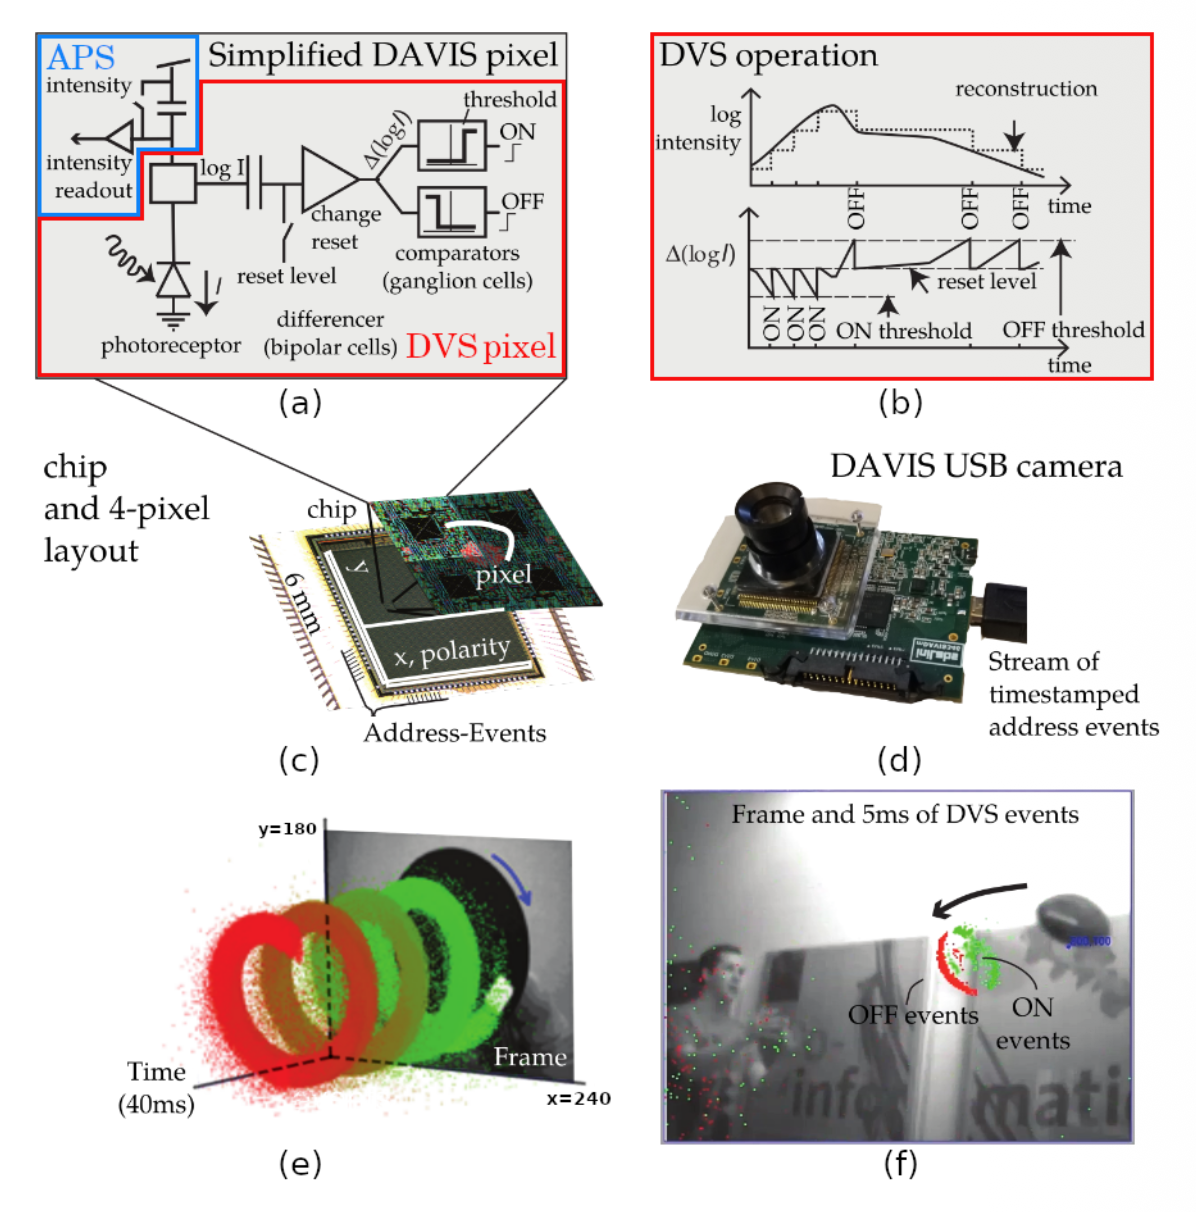
\includegraphics[width=0.75\textwidth]{images/fig_event_camera_principle.png}
    \caption[Operating principle of a dynamic vision sensor]{Operating principle of a Dynamic Vision Sensor (DVS). Each pixel independently and asynchronously fires an event when the change in log luminance exceeds a contrast threshold $C$, producing a stream of events $(x, y, t, p)$ with microsecond temporal resolution. Adapted from \cite{gallego2020event}.}
    \label{fig:dvs_principle}
\end{figure}

\section{Event Representations for Deep Learning}
A central challenge in applying deep learning to event camera data lies in bridging the gap between the asynchronous, sparse nature of event streams and the dense, regular tensor inputs expected by most neural network architectures. Several event representations have been developed to address this challenge, each embodying different trade-offs between information preservation and computational efficiency. 

The simplest representation is the event frame or event histogram, which accumulates events within a fixed time window into a two-dimensional grid where each pixel takes a value in {+1, 0, -1} based on event polarity \cite{gallego2020event}. While this representation is directly compatible with standard CNN architectures, it discards temporal information within the accumulation window, effectively reducing the event stream to a snapshot that loses the very temporal richness that distinguishes event cameras from conventional sensors. 

Voxel grids, proposed by Zhu et al. \cite{zhu2019unsupervised}, address this limitation by discretising the event stream into a three-dimensional spatio-temporal volume. Events are accumulated into B temporal bins, producing a tensor of dimensions B × H × W that preserves temporal ordering. This representation has been widely adopted in subsequent work, including the Events-to-Video (E2VID) reconstruction framework \cite{rebecq2019e2vid} and various optical flow estimation methods. The number of temporal bins B represents a tuneable parameter balancing temporal resolution against computational cost. 

\begin{figure}[htbp]
    \centering
    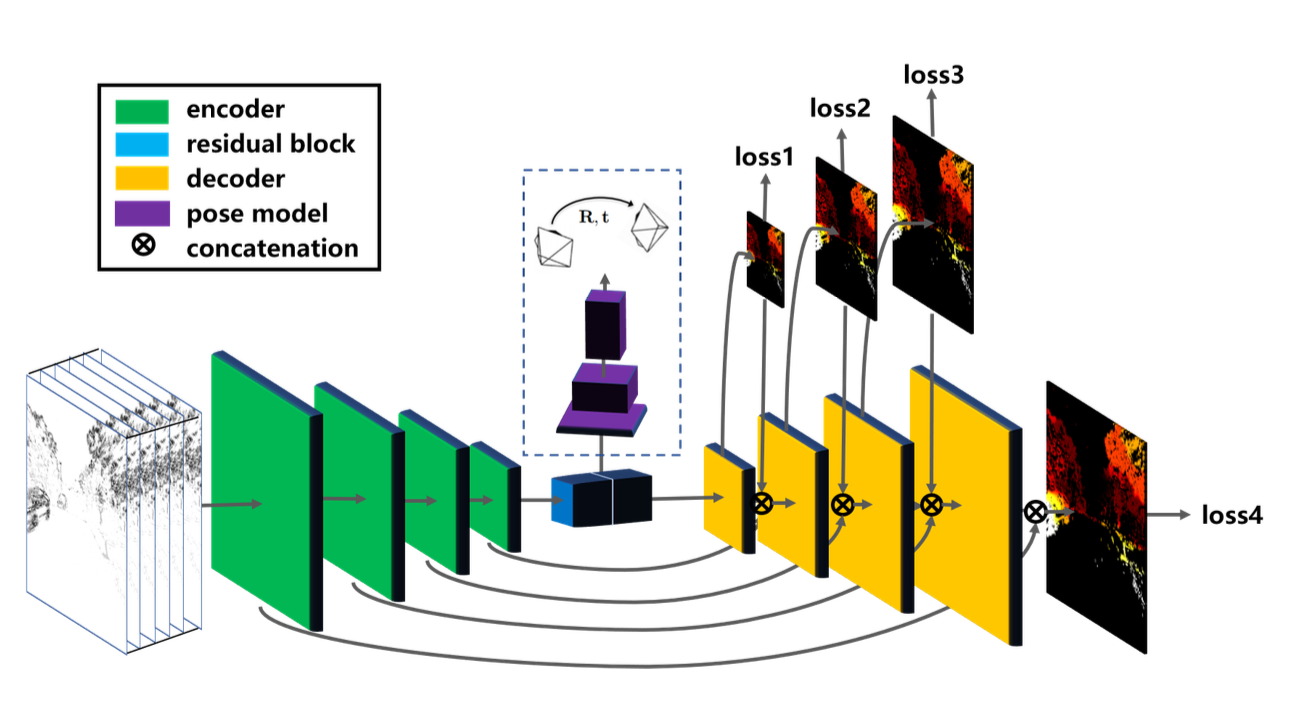
\includegraphics[width=0.75\textwidth]{images/fig_voxel_grid.png}
    \caption[Voxel grid event representation]{Voxel grid event representation. Events within a fixed time window are accumulated into $B$ temporal bins, producing a tensor of shape $B \times H \times W$ that preserves temporal ordering. Adapted from \cite{zhu2019unsupervised}.}
    \label{fig:voxel_grid}
\end{figure}

Time surfaces, introduced by Lagorce et al. \cite{lagorce2017hots}, offer an alternative encoding where each pixel stores an exponentially decaying function of the time since the last event at that location. This representation naturally encodes recency information and has been extended to Speed-Invariant Time Surfaces (SITS) that normalise for object velocity \cite{manderscheid2019speed}. Time surfaces are particularly effective for feature extraction and pattern recognition tasks, as they encode both spatial structure and temporal dynamics in a compact two-dimensional representation. 

Event Spike Tensors (ESTs), proposed by Gehrig et al. \cite{gehrig2019end}, sample the event stream using learned kernel functions, preserving temporal localisation with minimal information loss. Comparative studies have consistently demonstrated that representations retaining temporal localisation, such as voxel grids and ESTs, outperform simpler aggregation methods like event frames on downstream tasks \cite{gehrig2019end}. This finding underscores the importance of preserving the fine-grained temporal information inherent to event camera outputs. 

More recently, hybrid representations combining multiple channels of information have been explored. For instance, the Temporal Binary Representation packs the presence of events in successive sub-intervals into the bits of a single frame and has improved event-based action recognition \cite{innocenti2021temporal}. The choice of event representation remains an active area of research, with the optimal representation often being task-dependent. 

This work uses the stacked histogram of RVT \cite{gehrig2023recurrent}: per 50-ms window, event counts in ten temporal bins for each of the two polarities (Appendix~\ref{subsec:stacked_hist}). Like a voxel grid it preserves temporal ordering across bins, a property demonstrated to be critical for detection performance \cite{gehrig2019end}, and it is directly compatible with standard CNN and SSM-based backbones. It was not selected by a fresh comparison: it is part of the verified baseline's frozen pipeline (Section~\ref{sec:frozen_pipeline}), and changing it would confound the backbone comparison that is the subject of this thesis. The voxel grid proposed in the Thesis~A plan was therefore not adopted. Time surfaces, although compact, collapse temporal structure into a single 2D map and are less suited to multi-object detection tasks where simultaneous events at different locations must be disambiguated. ESTs offer higher temporal fidelity through learned kernels, but introduce additional parameters and training complexity that is difficult to justify given the computational constraints of onboard UAV deployment. 

Compact multi-channel encodings of this kind have shown promise for action recognition \cite{innocenti2021temporal}, but require careful engineering of the channel structure and have not been validated for detection on the Gen1 automotive dataset used in this work. The bin count $B = 10$ is that of the RVT preprocessing \cite{gehrig2023recurrent}, inherited with the rest of the frozen pipeline. 

\section{Deep Learning for Event-Based Object Detection}
Object detection from event camera data has attracted growing research attention \cite{zheng2023deep}. This review groups the approaches into four paradigms: frame-conversion methods that adapt standard detectors, spiking neural network (SNN) approaches, graph neural network (GNN) methods, and recurrent architectures that process events sequentially. 

\subsection{Frame-Conversion Approaches}
The most straightforward approach to event-based object detection converts event streams into frame-like representations and applies established detection architectures such as YOLO, SSD, or Faster R-CNN. Iacono et al. \cite{iacono2018towards} demonstrated on the iCub humanoid robot that event histograms can be processed by standard object detectors with reasonable accuracy, bootstrapping the event-based annotations from mature frame-based detectors. While this approach benefits from the maturity and optimisation of frame-based detection pipelines, it fundamentally fails to exploit the temporal continuity of the event stream, treating each accumulated frame independently. Furthermore, the frame accumulation step introduces latency that partially negates the low-latency advantage of event cameras. 

Large-scale automotive benchmarks followed: the Gen1 dataset of de Tournemire et al. \cite{detournemire2020large} and the 1Mpx dataset of Perot et al. \cite{perot2020learning}. Perot et al.'s detector, RED, already moves beyond per-window processing: ConvLSTM layers carry information across windows, and a temporal-consistency loss stabilises the predictions over time \cite{perot2020learning}. It belongs with the recurrent architectures discussed below.

\subsection{Spiking Neural Networks}
Spiking neural networks (SNNs) represent a bio-inspired approach that is architecturally well-matched to the asynchronous, binary nature of event camera outputs. In SNNs, information is encoded as discrete spikes rather than continuous activations, enabling highly energy-efficient computation on neuromorphic hardware \cite{roy2019towards}. The DT-LIF (Dual-Threshold Leaky Integrate-and-Fire) neuron model combined with the SSD detection framework, as proposed by Zhou et al. \cite{zhou2023dtlif}, demonstrated that SNNs can perform object detection from event data with significantly lower energy consumption than conventional neural networks. The dual-threshold mechanism improves the neuron's ability to encode temporal patterns by introducing separate thresholds for excitation and inhibition. 

More recently, the Hybrid Spiking Vision Transformer (HsVT) \cite{xu2025hybrid} has integrated spatial feature extraction with temporal spike-based processing, achieving competitive performance with fewer parameters and lower energy consumption than equivalent artificial neural networks. The key advantage of SNN-based detection for micro UAV applications lies in the potential for deployment on neuromorphic processors such as Intel's Loihi or SynSense's Speck chip, which offer orders-of-magnitude improvements in power efficiency compared to conventional GPUs \cite{synsense2026speck}. SNN training is complicated by the non-differentiability of spike generation, and for years spiking detectors lagged behind conventional architectures in accuracy; on Gen1 the most recent ones have closed that gap (Section~\ref{sec:snn_detection}). 

\subsection{Graph Neural Networks}
An alternative paradigm models the event stream as a spatio-temporal graph, where individual events serve as nodes connected to their spatial and temporal neighbours. Graph neural networks (GNNs) can then extract features from this naturally sparse representation without requiring conversion to dense tensors \cite{bi2019graph}. The Asynchronous Event-based GNN (AEGNN) framework \cite{schaefer2022aegnn} demonstrated that graph-based processing preserves the asynchronous nature of events while enabling efficient feature extraction through graph convolutions and pooling operations. The primary advantage of GNN approaches is their ability to process events at their native resolution without temporal binning, potentially preserving more information than frame-based methods. However, the irregular memory access patterns of graph operations can be challenging to optimise on conventional hardware, and scalability to high event rates remains an open problem. 

\subsection{Recurrent Architectures}
Recurrent neural networks (RNNs), particularly convolutional LSTMs and GRUs, have been widely applied to sequential event processing. Recurrent architectures naturally accumulate temporal context across event windows, making them well-suited for tasks requiring temporal reasoning \cite{rebecq2019e2vid}, \cite{cannici2019attention}. The E2VID framework \cite{rebecq2019e2vid}, while primarily targeting video reconstruction, demonstrated that a recurrent UNet encoder-decoder can effectively process temporal sequences of event representations. Detection frameworks have adopted recurrent feature extractors to build temporal context, from the ConvLSTM-based RED \cite{perot2020learning} to RVT \cite{gehrig2023recurrent}. 

The principal limitation of recurrent approaches for deployment on micro UAVs is their sequential processing requirement, which limits parallelisation and can create computational bottlenecks. Additionally, RNNs are known to struggle with very long temporal dependencies due to vanishing gradient problems, though gated variants partially mitigate this issue. Zubic et al. \cite{zubic2024state} report that RNN-based event detectors degrade sharply when deployed at inference frequencies other than their training frequency, a limitation that matters for the variable-rate nature of event camera data. 

\section{State Space Models: Architecture and Evolution}
State Space Models (SSMs) have recently emerged as a powerful class of sequence models that address many of the computational limitations of transformers and recurrent networks \cite{gu2022efficiently}. Rooted in control theory, SSMs model the relationship between an input sequence $u(t)$ and an output sequence $y(t)$ through a latent state $h(t)$ governed by a continuous-time linear dynamical system:

\begin{align}
    h'(t) &= Ah(t) + Bu(t) \\
    y(t) &= Ch(t) + Du(t)
\end{align}

where $A, B, C$, and $D$ are learnable parameter matrices \cite{gu2022efficiently}. This continuous-time formulation can be discretised at arbitrary time steps $\Delta t$ using methods such as the zero-order hold, enabling flexible adaptation to different sampling rates \cite{gu2022efficiently, zubic2024state}. 

The discretisation process transforms the continuous parameters $(A, B)$ into their discrete counterparts $(\overline{A}, \overline{B})$ using the step size $\Delta$:

\begin{equation}
    \overline{A} = \exp(\Delta A), \quad \overline{B} = (\exp(\Delta A) - I)A^{-1}B
\end{equation}

This allows the model to be computed as a linear recurrence, which is significantly more efficient for long sequences than the quadratic complexity of self-attention \cite{gu2023mamba, somvanshi2025from}.

The Structured State Space Sequence Model (S4), proposed by Gu et al. \cite{gu2022efficiently}, represented a breakthrough by introducing a special parameterisation of the state matrix A based on the HiPPO (High-order Polynomial Projection Operator) framework. This parameterisation enables the efficient computation of very long-range dependencies while maintaining linear computational complexity in sequence length. S4 achieved state-of-the-art results on the Long Range Arena benchmark, including the challenging Path-X task with sequence lengths of 16,384, and attained 91\% accuracy on sequential CIFAR-10 \cite{gu2022efficiently}. The S5 variant \cite{smith2023simplified} further simplified the architecture by employing a diagonal state structure with parallel scan mechanisms, eliminating the need for computationally expensive FFT operations while maintaining comparable performance. 

\section{Mamba and Selective State Spaces}
The Mamba architecture, proposed by Gu and Dao \cite{gu2023mamba}, introduced a critical innovation: selective state spaces. Unlike the time-invariant S4 model, Mamba makes the matrices $B$, $C$, and the discretisation step $\Delta$ input-dependent, enabling the model to selectively attend to or ignore different parts of the input sequence based on content \cite{gu2023mamba}. This is achieved by defining these parameters as functions of the input $x_t$:

\begin{align}
    B_t &= \text{Linear}_B(x_t) \\
    C_t &= \text{Linear}_C(x_t) \\
    \Delta_t &= \text{Softplus}(\text{Parameter}_\Delta + \text{Linear}_\Delta(x_t))
\end{align}

This selectivity is analogous to the gating mechanisms in LSTMs and GRUs but operates within the SSM framework while maintaining linear computational complexity \cite{gu2023mamba}. Input-dependent $\Delta_t$ allows for selective retention: a large $\Delta_t$ causes the state to decay rapidly (resetting the memory for irrelevant content), while a small $\Delta_t$ preserves long-range memory \cite{gu2023mamba, zubic2024state}. 

Because the parameters now vary with the input, the model can no longer be computed as a convolution. Mamba instead uses a hardware-aware algorithm that combines a parallel scan, kernel fusion and recomputation, giving about 5$\times$ higher inference throughput than Transformers of similar size while matching their quality in language modelling \cite{gu2023mamba}. Its successor, Mamba-2, recasts the selective scan through state-space duality and runs its core layer 2--8$\times$ faster than Mamba's \cite{dao2024transformers}. Such efficiencies are relevant to the size, weight, and power (SWaP) constraints of micro-UAV platforms.

\begin{figure}[htbp]
    \centering
    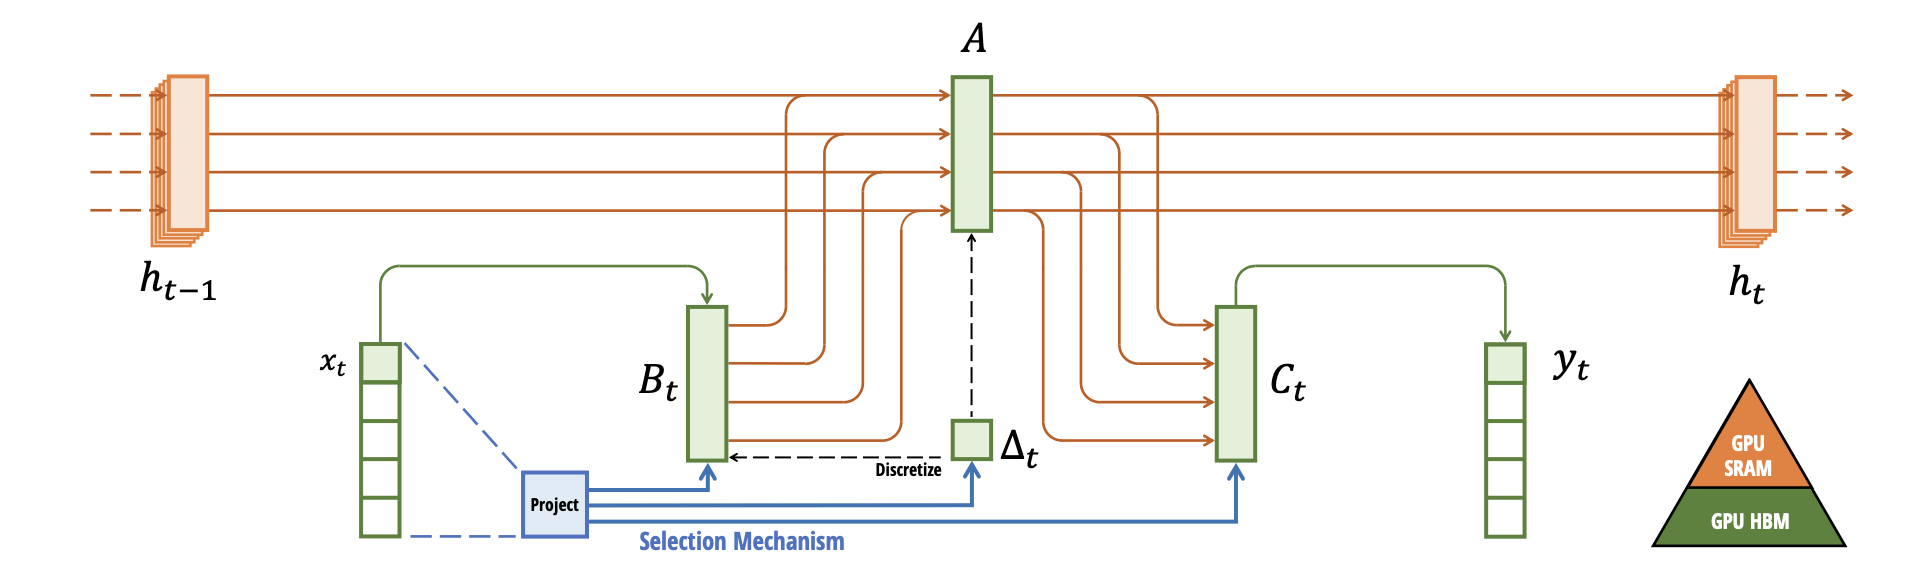
\includegraphics[width=0.85\textwidth]{images/fig_mamba_architecture.png}
    \caption[The Mamba selective state-space architecture]{The Mamba selective state space model architecture. Input-dependent parameters $\Delta_t$, $B_t$, and $C_t$ are computed as functions of the input $x_t$, enabling content-aware selective retention of long-range temporal context while maintaining linear computational complexity. Adapted from \cite{gu2023mamba}.}
    \label{fig:mamba_arch}
\end{figure}

The extension of SSMs to vision tasks has proceeded rapidly. Vision Mamba (Vim) \cite{zhu2024vision} proposed a vision backbone employing bidirectional Mamba blocks with position embeddings, achieving 2.8× faster inference than the DeiT transformer on ImageNet while using 86.8\% less GPU memory for high-resolution image processing. VMamba \cite{liu2024vmamba} introduced Visual State-Space (VSS) blocks with a 2D Selective Scan (SS2D) module that traverses image patches along multiple scan paths to capture two-dimensional spatial relationships. PlainMamba \cite{yang2024plainmamba} further explored non-hierarchical Mamba structures for visual recognition. These vision SSMs consistently demonstrate that the linear complexity of state space models can be leveraged for visual tasks without sacrificing the representational capacity needed for accurate perception. 

The computational advantages of SSMs are particularly relevant for micro UAV applications. The O(n) complexity of SSMs, compared to the O(n²) complexity of transformers, directly translates to reduced inference time and memory consumption. Furthermore, the continuous-time formulation of SSMs allows deployment at variable time scales without retraining, a property that Zubic et al. \cite{zubic2024state} report to be advantageous for event camera data, where the effective data rate varies with scene dynamics. A comprehensive survey by Somvanshi et al. \cite{somvanshi2025from} has catalogued the rapid evolution from S4 to Mamba and its variants, documenting the expanding application of SSMs across vision, language, and multi-modal tasks. 

\section{State Space Models for Event Camera Data}
The intersection of SSMs and event-based vision is a nascent but rapidly developing area. Zubic et al. \cite{zubic2024state} presented the first systematic investigation of SSMs for event camera data, published at CVPR 2024. Their work identified a fundamental limitation of existing deep learning approaches to event data: when trained at one temporal resolution (i.e., a specific ratio between the number of events and the number of forward passes of the network), models based on CNNs, RNNs, and transformers all exhibit significant performance degradation when deployed at different temporal resolutions. This is particularly problematic for event cameras, where the event rate naturally varies with scene dynamics. 

Zubic et al. \cite{zubic2024state} argued that SSMs, viewed as linear time-invariant (LTI) continuous-time systems, can be discretised at arbitrary step sizes without retraining. By rescaling a learnable timescale parameter by the ratio between training and inference frequencies, they report that their SSM-based models maintained performance across a range of deployment frequencies with minimal degradation (3.76 mAP drop versus >20 mAP for RNNs and transformers at higher frequencies). Furthermore, the SSM approach achieved 33\% faster training compared to equivalent recurrent models. If these results hold, SSMs are architecturally well suited to the temporal characteristics of event camera data; Section~\ref{subsec:f2} tests the reported compensation under the released checkpoint and code. 

The most influential baseline for event-based object detection is the Recurrent Vision Transformer (RVT) introduced by Gehrig and Scaramuzza \cite{gehrig2023recurrent}. RVT employs a four-stage hierarchical backbone combining convolutional priors with local and dilated global self-attention, using a ConvLSTM to carry hidden state across consecutive 50~ms windows \cite{gehrig2023recurrent}. A Feature Pyramid Network (FPN) and YOLOX detection head complete the pipeline \cite{gehrig2023recurrent}. 

RVT achieved $47.2$~mAP on the Gen1 automotive dataset with an inference latency below 12~ms, a five-fold reduction compared to prior art \cite{gehrig2023recurrent}. All subsequent SSM-based methods, including those explored in this work, benchmark against RVT, making it the de facto reference architecture for this thesis \cite{gehrig2023recurrent, zubic2024state, yang2025smamba}.

Zubic et al. \cite{zubic2024state}, described above, apply SSMs directly within the RVT framework for event-based object detection, achieving 47.71 mAP on Gen1 with S5 layers replacing the ConvLSTM. Critically, the SSM is used purely for inter-frame temporal aggregation; spatial feature extraction remains handled by Transformer attention blocks. The SSM variant employed is S5, a fixed-parameter (non-selective) model whose transition matrices do not depend on the input. 

Most recently, SMamba \cite{yang2025smamba} (AAAI 2025) advances the state of the art on Gen1 to 50.4 mAP by replacing the spatial Transformer stages of RVT with a Sparse Selective Mamba (S6) backbone. A Spatio-Temporal Continuity Assessment (STCA) module identifies informative tokens and discards noisy or inactive patches before the Mamba scan, reducing FLOPs by 23\% while improving accuracy. Inter-frame temporal context is still provided by a ConvLSTM, not Mamba. SMamba thus shows that a selective Mamba can replace attention for spatial feature extraction in event-based detection while reducing computation. 

Despite this progress, a consistent pattern emerges across the top-performing methods: each keeps inter-frame recurrence (an LSTM or SSM state carried across consecutive windows) and multi-scale FPN detection, and each changes several components of the RVT backbone at once. No prior work has compared a convolutional and a state-space spatial mixer under an otherwise identical backbone, temporal model and training pipeline. That controlled comparison, with a selective (Mamba) temporal recurrence in both models, is the primary architectural contribution of this thesis. The application of SSM-based event detection to micro-UAV platforms with SWaP constraints has no prior demonstration either, and remains outside the evaluation of this thesis (Section~\ref{sec:scope}).

\section{Event-Based Vision for UAV Navigation and Obstacle Avoidance}
The application of event cameras to UAV navigation has been an active area of research, driven by the sensor's inherent advantages for high-speed, low-latency perception. Pioneering work on event-based visual-inertial odometry by Rebecq et al. \cite{rebecq2017real} demonstrated that event cameras could provide accurate ego-motion estimation, a fundamental capability for UAV localisation. Their approach tracked features in motion-compensated event frames and fused them with inertial measurements in a keyframe-based nonlinear optimisation to estimate the 6-DOF pose, remaining robust under rapid motion and high dynamic range. 

Vidal et al. \cite{vidal2018ultimate} extended this work by fusing events, standard frames and inertial measurements in a single state-estimation pipeline (Ultimate SLAM). The fusion improved accuracy by 130\,\% over an events-only and by 85\,\% over a frames-only visual-inertial pipeline, and remained reliable in high-speed and high-dynamic-range scenes, including on a flying quadrotor. 

Falanga et al. \cite{falanga2020dynamic} presented a seminal contribution in event-based obstacle avoidance for quadrotors, building on their analysis of how perception latency limits the safe speed of a sense-and-avoid system \cite{falanga2019fast}. Their approach performed motion segmentation on the event stream to identify independently moving objects, then computed time-to-contact estimates to trigger avoidance manoeuvres. The system achieved an overall processing latency of approximately 3.5 milliseconds, enabling the quadrotor to avoid obstacles at relative speeds up to 10 m/s. Critically, their work demonstrated that event cameras could enable reactive obstacle avoidance at speeds far beyond the capabilities of frame-based perception systems, where the minimum achievable latency is bounded by the frame period (about 17--33~ms at 30--60 frames per second). 

Sanket et al. \cite{sanket2020evdodgenet} proposed EVDodge, an event-based dodging system tested on UAV platforms. Their approach demonstrated real-time obstacle avoidance using purely event-based perception, showing that the high temporal resolution of event cameras could be directly translated into improved avoidance performance. The system was validated both in simulation and on physical quadrotor platforms, confirming the practical feasibility of event-based avoidance systems. 

More recent work has explored bio-inspired processing pipelines for event-based UAV obstacle avoidance. Xu et al. \cite{li2024taming} proposed BioDrone, which processes stereo event cameras with a chiasm-inspired pipeline for fast event filtering and obstacle detection and a lateral-geniculate-nucleus-inspired matching algorithm for obstacle localisation, deployed on an FPGA through software--hardware co-design, and reported an obstacle detection rate of 96.1\%. Such co-designed pipelines are particularly relevant for micro UAVs, where the power budget is a primary constraint. 

Despite these advances, each of the surveyed approaches has notable limitations. The visual odometry and motion segmentation methods of Rebecq et al.\ \cite{rebecq2017real} and Falanga et al.\ \cite{falanga2020dynamic} use handcrafted features and geometric rules rather than learned representations, which limits how well they generalise to new environments. EVDodge \cite{sanket2020evdodgenet}, while shown to work on real hardware, uses a relatively shallow network that has not been tested under challenging conditions such as cluttered scenes or rapidly changing lighting. The bio-inspired pipeline of Xu et al.\ \cite{li2024taming} is attractive for its low latency, but relies on a co-designed FPGA implementation and hand-designed filtering and matching stages rather than the learned spatial features required for general object detection. Most importantly, none of these methods combine learned deep spatial features with a temporal model that can handle variable event rates, the core gap that this thesis addresses through its SSM-based detection architecture. 

\section{Contrast Maximisation and Motion Estimation from Events}
Gallego et al. \cite{gallego2018unifying} proposed a unifying contrast maximisation framework for event-based vision that provides a principled approach to estimating motion, depth, and optical flow from events. The core idea is to warp events according to a candidate motion model and measure the contrast (sharpness) of the resulting warped event image; the motion parameters that maximise contrast correspond to the true motion. This framework elegantly handles the data association problem inherent in event-based motion estimation without requiring explicit feature matching or appearance information. 

The contrast maximisation principle has been extended and refined by subsequent work. Shiba et al. \cite{shiba2024secrets} applied it to dense optical flow, depth, and ego-motion estimation, introducing multi-scale approaches to improve convergence and better handle occlusions. Self-supervised learning-based optical flow methods, such as EV-FlowNet \cite{zhu2018evflownet}, have also been developed, using photometric losses as supervisory signals to learn event-to-flow mappings without requiring ground truth annotations. These motion estimation capabilities are directly relevant to obstacle avoidance, as optical flow and time-to-contact can be used to identify and respond to approaching obstacles.

\section{Event Camera Datasets and Benchmarks}
The availability of standardised datasets has been instrumental in advancing event-based vision research. Several benchmark datasets are relevant to the object detection and navigation tasks considered in this thesis. 

The DSEC dataset \cite{gehrig2021dsec}, developed at the University of Zurich, provides high-resolution stereo event camera data captured using Prophesee Gen3.1 sensors with a 60 cm baseline, complemented by global shutter colour cameras and LiDAR ground truth. DSEC covers a range of driving scenarios under both favourable and challenging illumination conditions, making it a valuable benchmark for event-based depth estimation and optical flow. 

The MVSEC (Multi Vehicle Stereo Event Camera) dataset \cite{zhu2018multivehicle} uses DAVIS346B stereo pairs with a 10 cm baseline, providing synchronised event, frame, IMU, and LiDAR data. MVSEC includes sequences from indoor flying, outdoor driving, and motorcycle scenarios, offering diverse conditions for evaluating perception algorithms. 

For object detection specifically, the Gen1 \cite{detournemire2020large} and 1Mpx \cite{perot2020learning} datasets provide large-scale automotive event recordings from Prophesee cameras with bounding-box annotations: cars and pedestrians in Gen1, and pedestrians, two-wheelers and cars in 1Mpx. The N-Caltech101 dataset \cite{orchard2015converting} provides an event camera version of the Caltech101 classification benchmark, created by displaying images on a monitor in front of a DVS camera executing saccadic movements. While primarily a classification benchmark, N-Caltech101 has been widely used for evaluating event representation and feature extraction methods. 

A significant gap exists in available datasets for UAV-specific scenarios. Most event camera datasets target automotive applications, and there are limited publicly available datasets that capture the specific challenges of micro UAV navigation: rapid ego-motion, indoor environments, small obstacles, and the particular motion patterns characteristic of rotary-wing flight. Addressing this dataset gap remains an open challenge for UAV-specific event-based perception research. For the purposes of this thesis, the primary evaluation is conducted on the Gen1 automotive dataset, which provides a well-established benchmark for detection performance. Obstacle avoidance is treated as a motivating application rather than a directly evaluated system; the trained detection model represents the core perceptual component that such a system would require. Extension to UAV-specific scenarios, potentially through synthetic data generation in open-source simulators such as Gazebo with event camera emulation, is identified as a direction for future work subject to hardware and time constraints. 

\section{Computational Constraints and Obstacle Avoidance for Micro UAVs}
Micro UAVs in the sub-250 gram class face severe SWaP constraints that fundamentally shape the design of onboard perception systems. Typical computational platforms for nano- and micro-UAVs are milliwatt-class microcontrollers and parallel ultra-low-power processors, on which even a compact navigation network runs at only about 9--13 frames per second \cite{niculescu2021improving}; they are orders of magnitude less capable than the GPU-equipped systems used to train and evaluate most deep learning models. This disparity between training and deployment hardware necessitates either highly efficient model architectures, hardware acceleration, or offloading computation to a ground station at the cost of communication latency. 

Several approaches to obstacle avoidance on resource-constrained platforms have been explored. Traditional methods based on optical flow divergence, time-to-contact estimation or event-based motion segmentation provide computationally lightweight avoidance capabilities but lack the ability to classify specific obstacles \cite{decroon2016monocular, falanga2020dynamic}. Model predictive control (MPC) approaches can generate optimal avoidance trajectories but require real-time environmental perception as input. Cooperative approaches, where a less-equipped micro UAV receives guidance from a sensor-rich companion \cite{pritzl2024drones}, offer a pragmatic solution but introduce communication dependencies. 

The emergence of neuromorphic processing hardware offers a potential path to efficient onboard perception. The SynSense Speck chip \cite{synsense2026speck} integrates a dynamic vision sensor with a fully asynchronous spiking neural network processor, achieving real-time event processing with idle power consumption below 1 mW. Similarly, Intel's Loihi processors support on-chip learning and efficient SNN inference \cite{davies2021advancing}, and Loihi~2 adds programmable neuron models and graded spikes \cite{orchard2021efficient}. These platforms are particularly well-suited to processing event camera data, as they natively handle the sparse, asynchronous data format. However, the software ecosystem for neuromorphic processors remains immature compared to conventional deep learning frameworks, and mapping complex detection architectures onto neuromorphic hardware remains an active research challenge. 

The linear complexity and inherent efficiency of SSM-based architectures position them as strong candidates for deployment on the limited computational resources available on micro UAVs. Unlike transformer-based models, whose memory and computation grow quadratically with sequence length, SSMs process long event sequences with a fixed-size recurrent state, although that state can be large (Section~\ref{sec:efficiency}). Combined with model compression techniques such as quantisation and pruning, SSM architectures may enable real-time object detection on platforms that cannot support transformer or large CNN inference. 

\section{Identification of Research Gaps}
\label{sec:gaps_thesisA}
The preceding review reveals several interconnected research gaps that this thesis aims to address: 

Gap 1: Pure selective Mamba for event-based object detection. Existing SSM-based detection methods integrate SSM layers into Transformer backbones \cite{zubic2024state} or employ selective Mamba within sparse-attention hybrid frameworks \cite{yang2025smamba}. In both cases, inter-frame recurrence is maintained via ConvLSTM or SSM hidden state passed across consecutive windows. No prior work has evaluated a fully recurrence-free, convolutional-free selective Mamba architecture for event-based detection, nor conducted a controlled ablation comparing a CNN-SSM hybrid against a pure SSM model under identical loss functions, detection heads, and training protocols. Such a comparison is required to isolate the contribution of the spatial feature extractor from all other architectural variables. 

Gap 2: Integrated detection and avoidance for micro UAVs. Existing event-based UAV obstacle avoidance systems \cite{falanga2020dynamic, sanket2020evdodgenet} predominantly employ reactive strategies based on optical flow or motion segmentation, without explicit object detection. Conversely, event-based detection methods \cite{perot2020learning,gehrig2023recurrent} have been evaluated primarily on automotive benchmarks. An integrated system that combines SSM-based object detection with obstacle avoidance control, specifically designed for micro UAV deployment, has not been demonstrated. 

Gap 3: Computational efficiency benchmarking for onboard deployment. While the theoretical computational advantages of SSMs over transformers and RNNs are well-established, systematic benchmarking of SSM inference latency, memory consumption, and energy usage on the constrained hardware platforms typical of micro UAVs has not been conducted. Understanding the practical deployment characteristics of SSM-based detection models is essential for validating their suitability for this application domain. 

Gap 4: Variable-rate event processing for obstacle avoidance. The unique ability of SSMs to generalise across temporal resolutions \cite{zubic2024state} has not been exploited in the context of obstacle avoidance, where the event rate varies dramatically with UAV speed and scene complexity. An adaptive processing framework that adjusts its temporal resolution based on event rate while maintaining detection performance could significantly improve both efficiency and robustness. 

As registered in Thesis~A, these gaps defined the research space as developing and evaluating SSM-based architectures for event-based object detection and obstacle avoidance on micro UAVs, with a focus on computational efficiency, temporal adaptability and practical deployability. Section~\ref{sec:gaps_revisited} revises them after the scope change. 

% --- Chapter 3: Methodology ---

\section{Spiking Neural Networks for Event-Based Detection}
\label{sec:snn_detection}
Directly-trained spiking neural networks (SNNs) are an established family on this benchmark and the
comparison class for the neuromorphic strand of this thesis. They are trained with surrogate
gradients~\cite{neftci2019surrogate}: the non-differentiable spike function is kept in the forward pass
and replaced by a smooth surrogate derivative in the backward pass, which makes back-propagation through
time applicable to networks of spiking neurons. Table~\ref{tab:snn_landscape} places the spiking detectors
reported on Gen1 against the non-spiking models of this thesis.

\begin{table}[htbp]
\centering
\small
\caption[Spiking and non-spiking detectors on Gen1]{Object detection on Prophesee Gen1, COCO mAP@[0.50:0.95] on the test split. Ranges span the
reported model sizes. $T\times D$: timesteps $\times$ virtual timesteps of integer-valued training
($D=1$: binary spikes throughout). SpikeDet is a preprint (version 5, 2026); its first version, under
the title SpikSSD, reported 40.8.}
\label{tab:snn_landscape}
\begin{tabularx}{\textwidth}{@{}l>{\raggedright\arraybackslash}Xccl@{}}
\toprule
\textbf{Model} & \textbf{Type} & \textbf{$T\times D$} & \textbf{mAP} & \textbf{Venue} \\
\midrule
RVT \cite{gehrig2023recurrent}        & ANN (attention, ConvLSTM) & --- & 47.2 & CVPR 2023 \\
S5-RVT \cite{zubic2024state}          & ANN (attention, S5)       & --- & 47.7 & CVPR 2024 \\
SMamba \cite{yang2025smamba}          & ANN (sparse Mamba, ConvLSTM) & --- & 50.4 & AAAI 2025 \\
EventSSM (this work)                  & ANN (convolution, Mamba-2) & --- & 46.2 & --- \\
PureSSM (this work)                   & ANN (BiMamba, Mamba-2)    & --- & 46.4 & --- \\
\midrule
HsVT \cite{xu2025hybrid}              & hybrid (spiking temporal block) & --- & 44.9--47.8 & ICML 2025 \\
SpikeDet \cite{fan2025spikedet}       & SNN, integer-valued       & $5\times1$, $4\times2$ & 46.5--47.6 & preprint \\
EAS-SNN \cite{wang2024eas}            & SNN, recurrent            & $3$ & 37.2--40.9 & ECCV 2024 \\
SpikeYOLO \cite{luo2024integer}       & SNN, integer-valued       & $5\times1$, $4\times2$ & 38.5--40.4 & ECCV 2024 \\
EMS-YOLO \cite{su2023deep}            & SNN                       & $5$ & 26.7--31.0 & ICCV 2023 \\
\bottomrule
\end{tabularx}
\end{table}

Two observations follow. First, the accuracy gap between spiking and non-spiking detectors on Gen1 has
closed. EMS-YOLO, the first deep directly-trained spiking detector~\cite{su2023deep}, reached 31.0 in 2023,
16.7~mAP below S5-RVT; the strongest recent spiking detectors, SpikeDet~\cite{fan2025spikedet} and
HsVT~\cite{xu2025hybrid}, report 47.6 and 47.8, level with S5-RVT and above the own models of this thesis.
On this benchmark a spiking detector is therefore no longer necessarily a less accurate one, and the case
for the neuromorphic strand rests on energy and deployment rather than accuracy.

Second, the mechanisms behind that progress are identifiable, and both are native to a state-space neuron.
\emph{More information per spike:} SpikeYOLO's I-LIF neuron emits integer values in $\{0,\dots,D\}$ during
training and, at inference, expands each integer into $D$ binary spikes over virtual timesteps, so that
inference remains spike-driven (binary, accumulate-only) while training sees a multi-bit
signal~\cite{luo2024integer}. SpikeDet uses the same integer-valued scheme, and for both detectors the
$4\times2$ configuration, with fewer timesteps each carrying a two-level value, outperforms $5\times1$. \emph{Temporal state:}
EAS-SNN uses recurrent convolutional SNNs with temporal memory as an adaptive event sampler~\cite{wang2024eas},
and HsVT combines LSTM blocks with a spiking temporal feature-extraction block on a MaxViT spatial
backbone~\cite{xu2025hybrid}. HsVT is the closest design point to the spiking model of this thesis: it keeps
spatial processing in non-spiking form and spikes along time. A state-space neuron supplies both mechanisms
by construction, since its state is a carried, multi-valued memory and the graded readout of
Section~\ref{subsec:readout_modes} is the per-neuron analogue of an integer-valued spike. EMS-YOLO and
SpikeYOLO also report an ANN of equivalent architecture, so the overall cost of spiking is known for those
designs; where that cost comes from is not reported.

\section{Spiking State Space Models}
\label{sec:spiking_ssm}
A discretised diagonal state-space model and a leaky integrate-and-fire neuron are the same linear
recurrence with different readouts. Consider one state dimension of a diagonal SSM with decay $a<0$,
input weight $b$, output weight $c$ and step $\Delta$, discretised with a zero-order hold:
\begin{equation}
  h_t = \bar a\, h_{t-1} + \bar b\, u_t, \qquad y_t = c\, h_t, \qquad
  \bar a = e^{\Delta a}, \quad \bar b = \frac{e^{\Delta a}-1}{a}\, b .
  \label{eq:ssm_scalar}
\end{equation}
The discrete LIF neuron of Equations~\eqref{eq:lif_integrate}--\eqref{eq:lif_reset} integrates its input
$x_t$ as $m_t = \beta m_{t-1} + x_t$. With $\beta = \bar a$ and $x_t = \bar b u_t$ the membrane potential
$m_t$ \emph{is} the SSM state $h_t$, and the leak is a discretised decay. The neuron differs in two
respects only. Its readout is a threshold, $s_t = \Theta(m_t - \vartheta)$, instead of a linear map; and its
reset, $m_t \leftarrow m_t - s_t\vartheta$, feeds the output back into the state. The second difference is
the consequential one. Without reset the recurrence is linear and can be evaluated with a parallel scan, as
SSMs are during training; with reset the state depends on its own thresholded past, and the recurrence must
be unrolled sequentially. Much of the spiking-SSM literature consists of ways around that obstacle,
summarised in Table~\ref{tab:spiking_ssm}.

\begin{table}[htbp]
\centering
\small
\caption[Spiking state-space models]{Spiking state-space models. All except the last row target one-dimensional sequence tasks.}
\label{tab:spiking_ssm}
\begin{tabularx}{\textwidth}{@{}l>{\raggedright\arraybackslash}X>{\raggedright\arraybackslash}Xl@{}}
\toprule
\textbf{Work} & \textbf{How spiking enters} & \textbf{Parallel training} & \textbf{Task} \\
\midrule
SpikingSSMs \cite{shen2025spikingssms} & spiking neurons with learnable thresholds driven by an S4D-type SSM &
  a small network predicts the after-reset membrane & LRA, WikiText-103 \\
SPikE-SSM \cite{zhong2024spike} & reset-refractory neuron, trainable thresholds & boundary compression of
  the membrane & LRA, WikiText-103 \\
P-SpikeSSM \cite{bal2025p} & spikes sampled stochastically from an SSM-based neuron & sampling replaces
  sequential spike generation & long-range tasks \\
SiLIF \cite{fabre2025silif} & the neuron is a two-state SSM with S4-style parametrisation & --- (surrogate
  gradients through time) & speech \\
Spiking-S4 \cite{du2023spiking} & spiking neurons combined with an S4 model & --- & speech enhancement \\
SpikeMba \cite{li2024spikemba} & spiking saliency detector for proposals; Mamba non-spiking & --- &
  video grounding \\
\midrule
This thesis & LIF readout on the output of a selective (Mamba-2) temporal block & SSM scan unchanged;
  readout unrolled over the clip & event detection \\
\bottomrule
\end{tabularx}
\end{table}

SpikingSSMs~\cite{shen2025spikingssms} train a lightweight surrogate dynamic network to predict the
after-reset membrane potential, which restores parallel training with orders-of-magnitude speed-ups over
iterative unrolling, and report performance competitive with non-spiking SSMs at about 90\,\% network
sparsity. SPikE-SSM~\cite{zhong2024spike} accelerates the same computation by compressing the membrane
dynamics between spike boundaries and adds a reset-refractory neuron with trainable thresholds.
P-SpikeSSM~\cite{bal2025p} avoids sequential spike generation altogether by sampling spikes stochastically
from an SSM-based neuronal model. SiLIF~\cite{fabre2025silif} takes the correspondence of
Equation~\eqref{eq:ssm_scalar} in the other direction: it makes it exact for a two-state adaptive neuron and
gives the neuron an S4-style parametrisation (decays trained in logarithmic form, a learnable per-neuron step,
and a complex-valued variant with oscillatory dynamics), reporting state-of-the-art accuracy among spiking
neuron models on speech. Spiking-S4~\cite{du2023spiking} combines S4 with spiking neurons for speech
enhancement at reduced parameter and FLOP counts.

Two limitations of this literature matter here. First, it targets one-dimensional sequence tasks: long-range
benchmarks, language modelling and speech. Second, it is built on linear time-invariant SSMs (S4, S4D), whose
decay does not depend on the input. The only selective model in Table~\ref{tab:spiking_ssm}, SpikeMba, keeps
Mamba itself non-spiking and uses spikes only for proposal generation~\cite{li2024spikemba}. In a selective
SSM the decay $\bar a_t = e^{\Delta_t a}$ varies with the input at every step. The recurrence is still linear
in the state, so a spiking \emph{readout} placed after the scan, as in this thesis, leaves the scan exact and
parallel; making the selective state itself spike, with a reset inside the scan, would require one of the
parallel-training devices above to be extended to input-dependent decays.

\section{Neuromorphic Hardware and the Deployment Path}
\label{sec:neuromorphic_hw}
Neuromorphic processors execute spiking networks in an event-driven manner: computation and
communication happen only when spikes arrive, so energy scales with activity rather than with the size of
the input~\cite{davies2021advancing}. Two features of Intel's Loihi~2 matter for state-space models.
Its neuron models are programmable in microcode rather than fixed to a LIF primitive, so any small
per-neuron recurrence, including the state update of a diagonal SSM, can be implemented directly; and it
supports graded spikes, which carry an integer payload rather than a single bit~\cite{orchard2021efficient},
the hardware counterpart of integer-valued and graded readouts.

Meyer et al.~\cite{meyer2024diagonal} gave the first implementation of an SSM on neuromorphic hardware,
mapping S4D to Loihi~2. The comparison with an NVIDIA Jetson Orin Nano depends on the processing mode. In
offline, batched, sample-by-sample processing the Jetson performed better; in token-by-token processing,
Loihi~2 consumed about 1000 times less energy, with 75 times lower latency and 75 times higher throughput,
than a recurrent S4D implementation on the Jetson. Token-by-token processing is exactly the regime of a
streaming event camera, which is why this result motivates the neuromorphic strand. It was obtained for a
linear time-invariant SSM on one-dimensional sequence benchmarks; a selective SSM, whose decay must be
recomputed from the input at every step, and a two-dimensional detection backbone remain untested on such
hardware. Other neuromorphic substrates take a different route: SynSense's Speck integrates an event sensor
and a spiking processor on one chip~\cite{synsense2026speck}.

Energy figures for spiking detectors run on GPUs are estimates, not measurements. The convention in the
detection literature is to count synaptic operations and multiply them by a per-operation energy, typically
0.9~pJ for a 32-bit floating-point accumulate against 4.6~pJ for a multiply--accumulate at
45~nm~\cite{horowitz2014computing,su2023deep,luo2024integer}. Such estimates ignore memory access and data
movement, which dominate energy on real hardware, so they rank designs rather than predict silicon
consumption; measured results such as Meyer et al.'s are rare by comparison.

The software path is in transition. Intel archived its Lava framework on 13 May 2026, stated that it will
no longer maintain it, and announced a successor SDK without a public timeline~\cite{intel2026lava}. The
Neuromorphic Intermediate Representation (NIR) defines a common set of computational primitives through
which models can be exchanged between simulators and neuromorphic hardware~\cite{pedersen2024neuromorphic},
and is used in this thesis as the export boundary for that reason.

\section{Research Gaps Revisited}
\label{sec:gaps_revisited}
The gap list of Section~\ref{sec:gaps_thesisA}, carried over from Thesis~A, assumed an integrated
detection-and-avoidance system. After the scope change (Section~\ref{sec:scope_change}) its second gap,
integrated detection and avoidance, is retired; its fourth, variable-rate processing for avoidance,
survives as the rate robustness of the detector alone. Its first gap asked for a recurrence-free,
convolution-free selective Mamba detector. The models built here keep a selective temporal recurrence ---
an asset, as the rate-robustness results show --- and a strided convolutional stem, so that gap is
restated as Gap~A below. Its third gap, benchmarking on constrained hardware, is addressed only in part:
latency, energy and memory are measured for every model, but on a desktop GPU rather than embedded
hardware (Section~\ref{sec:efficiency}). The gaps this thesis addresses are narrower
and better defended than those originally proposed.

\textbf{Gap~A: the isolated effect of the spatial mixer.} Published SSM detectors change several things at
once. S5-RVT replaces the temporal mixer of an attention backbone~\cite{zubic2024state}; SMamba replaces the
spatial attention with a sparse Mamba, adds token selection and keeps a ConvLSTM in
time~\cite{yang2025smamba}. Neither isolates what the spatial mixer itself contributes. This thesis
measures it with two detectors that differ only in that component (Section~\ref{sec:acc_results}).

\textbf{Gap~B: rate robustness under the published artefacts.} The temporal generalisation of SSM detectors
has been attributed to inference-time rescaling of the discretisation step~\cite{zubic2024state}. Whether
the reported high-rate results can be reproduced from the released checkpoint and code, and how the
robustness behaves under a fixed cadence versus a true rate change, had not been examined
(Section~\ref{sec:robustness}).

\textbf{Gap~C: where the cost of spiking comes from.} Spiking detectors have reached the accuracy of
non-spiking ones on Gen1 (Table~\ref{tab:snn_landscape}), and spiking SSMs exist for sequence tasks
(Table~\ref{tab:spiking_ssm}). To the author's knowledge, no surveyed work combines a selective state-space
temporal core with spiking for event-based detection, and none decomposes the cost of spiking into the cost
of the neuron dynamics, of sparsity and of binarisation against a non-spiking twin trained through an
identical pipeline. The three readouts of Section~\ref{subsec:readout_modes}, which share one membrane, are
designed to measure exactly that decomposition (Section~\ref{sec:spiking_results}).

\chapter{Methodology}
\label{ch:method}
\guide{70}{
  \item What the chapter covers, in the order of its sections.
  \item The governing principle: only the backbone changes between models.
}
This chapter describes how the detectors were built, trained and evaluated.
Section~\ref{sec:repr} introduces the event representation and Section~\ref{sec:frozen_pipeline} the
detection pipeline shared by every model. Section~\ref{sec:models} describes the four models,
Sections~\ref{sec:dataset} and~\ref{sec:training} the data and the training recipe, and
Section~\ref{sec:eval_protocol} how accuracy, robustness and efficiency were measured. One principle
governs all of it: only the backbone changes from one model to the next.

\section{Event Representation}
\label{sec:repr}
\guide{120}{
  \item Events are grouped into 50-ms windows; counted per pixel, per polarity and in 10 time bins $\rightarrow$ 20 channels, shape $(20, 240, 304)$.
  \item Counts capped at 10 (formula in Appendix~\ref{app:maths}); zero-padded to $(20, 256, 320)$ so every stride divides it; feature maps $32\times40$, $16\times20$, $8\times10$ at strides 8, 16, 32.
  \item Sparsity: about 1.5\,\% non-zero (0.2--4.0\,\% per recording); the cap affects about 0.2\,\% of the non-zero entries.
  \item Cite RVT~\cite{gehrig2023recurrent}. Do not call it a voxel grid.
}
Every model consumes the stacked-histogram representation of RVT~\cite{gehrig2023recurrent}. The event
stream is cut into consecutive 50-ms windows, and within each window the events are counted per pixel,
separately for the two polarities and in ten equal time bins, which gives a tensor of $2\times10=20$
channels at the sensor's resolution, $(20, 240, 304)$
(Equations~\eqref{eq:sh_bin}--\eqref{eq:sh_count}, Appendix~\ref{app:maths}). Counts are capped at 10, and
the pipeline zero-pads the tensor to $(20, 256, 320)$ so that every downsampling stride divides it; the
feature maps passed to the detection neck are then $32\times40$, $16\times20$ and $8\times10$ at strides
8, 16 and 32. The representation is sparse: over 40 frames from each of 20 randomly drawn test recordings,
1.5\,\% of its entries are non-zero on average (between 0.2 and 4.0\,\% per recording, depending on scene
activity), and the cap is reached by only about 0.2\,\% of the non-zero entries.

\guide{90}{
  \item It was not chosen by a new comparison: it is the baseline's frozen input, and changing it would add a second variable.
  \item Point to Chapter~\ref{ch:lit} for the alternatives instead of repeating them.
  \item Consequences: one prediction per window (20\,Hz); latency cannot be shorter than the window.
  \item The voxel grid of Thesis~A was not used (one sentence).
}
The representation was not selected by a new comparison. It is the input of the verified S5-RVT
pipeline, and changing it would add a second variable to a study whose purpose is to vary only the
backbone; the alternatives are reviewed in Chapter~\ref{ch:lit}. The choice has two consequences that
the rest of the thesis carries. The detector makes one prediction per window, at 20\,Hz, and its
latency cannot be shorter than the window (Section~\ref{sec:latency_window}). The voxel grid proposed in
Thesis~A was accordingly not used.

\section{The Frozen Detection Pipeline}
\label{sec:frozen_pipeline}
\guide{160}{
  \item Reused unmodified: data pipeline, YOLO-PAFPN neck, YOLOX head, loss and label assignment, Prophesee evaluator, PyTorch Lightning training loop.
  \item How a backbone is swapped without editing the baseline code: Hydra configuration and a registration hook.
  \item Why this makes the comparison controlled; EventSSM vs PureSSM differ only in the spatial mixer (with its initialisation).
  \item What still differs from the published baseline: both mixers, batch 4 vs 8, bf16 vs 32-bit. Point to Figure~\ref{fig:spiking_arch}(a).
}
The methodological core of the thesis is that the detection pipeline around the backbone never changes.
Every model reuses the verified S5-RVT/RVT code base without modification: the data pipeline, the
YOLO-PAFPN neck, the YOLOX detection head~\cite{ge2021yolox} with its loss and label assignment, the
Prophesee evaluator and the PyTorch Lightning training loop. A new backbone enters through the Hydra
configuration and a registration hook that selects it by name, so the baseline's own code is never
edited. Figure~\ref{fig:spiking_arch}(a) shows the shared pipeline. Because only the backbone changes,
a difference between two models is attributable to their backbones, and between EventSSM and PureSSM,
which differ only in the spatial mixer and its initialisation, to that one component. The comparison
with the published baseline is looser: both mixers of its backbone differ from those of the own models,
and the own models were trained with batch size 4 and bf16 mixed precision rather than 8 and 32-bit
(Section~\ref{sec:training}).

\begin{figure}[htbp]
    \centering
    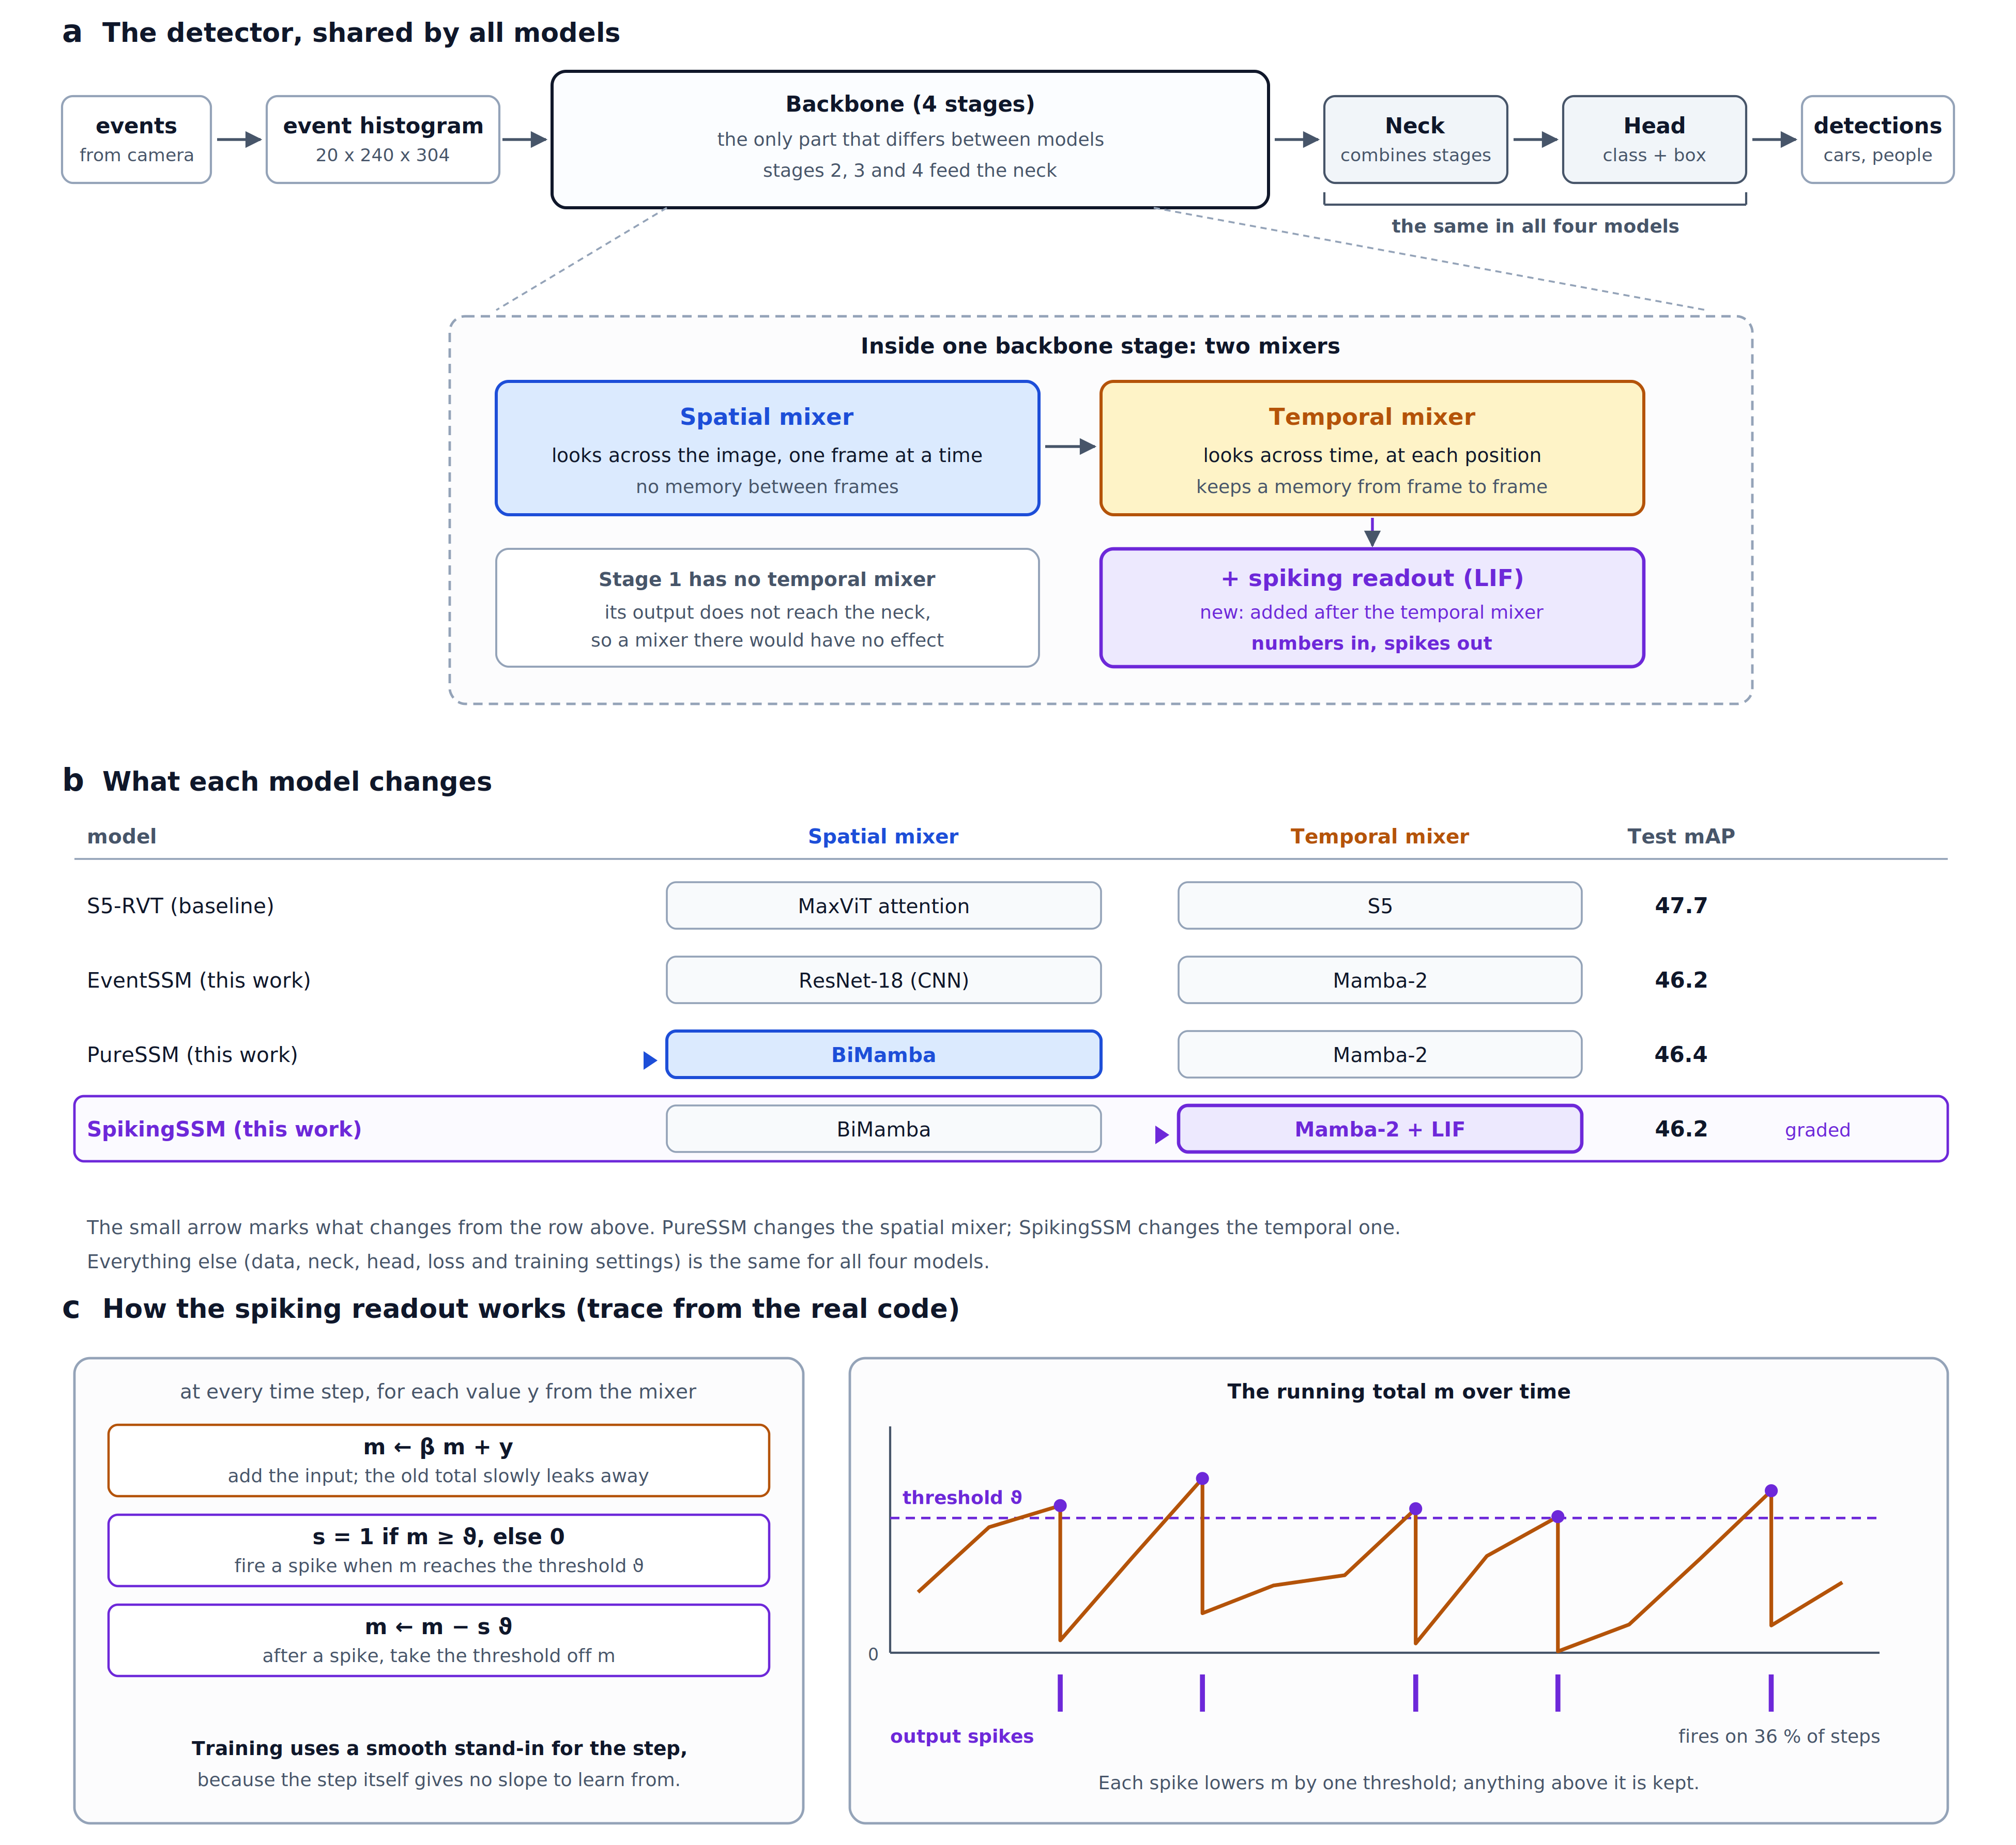
\includegraphics[width=\textwidth]{images/fig_spiking_architecture.png}
    \caption[Detector pipeline, mixing axes and LIF readout]{(a) The shared detector pipeline. The backbone is the only part that differs between
    models; the neck, head, loss, data pipeline and evaluator are frozen. Within a backbone stage
    there are two orthogonal mixing axes: a \emph{spatial} mixer acting within a frame (time folded
    into the batch, stateless) and a \emph{temporal} mixer acting across frames at each pixel (causal,
    state carried across clips). (b) Where each model intervenes: PureSSM changes the spatial axis,
    the spiking model changes the temporal one. (c) The LIF readout; the membrane trace is generated
    by executing the implementation itself rather than drawn by hand.}
    \label{fig:spiking_arch}
\end{figure}

\subsection{Neck, Head and Loss}
\label{subsec:neck_head}
\guide{120}{
  \item PAFPN: top-down then bottom-up fusion of the stride-8/16/32 features of stages 2--4.
  \item YOLOX: decoupled, anchor-free; objectness, class and box per cell; SimOTA dynamic label assignment.
  \item The loss as an equation, with its terms named.
  \item Correct the Thesis~A description (FCOS, focal, GIoU) in one sentence.
}
The neck is a YOLO-PAFPN~\cite{ge2021yolox}, which fuses the stride-8, 16 and 32 features of backbone
stages 2--4 first top-down and then bottom-up, so that every output scale combines fine localisation with
coarse context. The YOLOX head~\cite{ge2021yolox} is decoupled and anchor-free: at every cell of each scale
it predicts an objectness score, class scores and a box, and the SimOTA strategy assigns ground-truth boxes
to cells dynamically during training. The loss is
\begin{equation}
  \mathcal{L} \;=\; \mathcal{L}^{\mathrm{BCE}}_{\mathrm{obj}} + \mathcal{L}^{\mathrm{BCE}}_{\mathrm{cls}}
  + 5\,\big(1 - \mathrm{IoU}^2\big),
  \label{eq:loss}
\end{equation}
binary cross-entropy for objectness and class, and an IoU loss on the matched boxes with weight 5. The
Thesis~A report described the head and loss as FCOS with focal and GIoU losses; the code audit of this
project found the YOLOX configuration above, which is the one used for every model.

\subsection{The Two Mixing Axes}
\label{subsec:two_axes}
\guide{190}{
  \item Spatial mixer: within a frame, time folded into the batch, $(L\cdot B, C, H, W)$, stateless.
  \item Temporal mixer: along time at each location, $(B\cdot H\cdot W, L, C)$, causal, state carried across clips.
  \item Orthogonal axes $\Rightarrow$ each can be changed alone.
  \item Temporal blocks only on stages 2--4, as taps (the next spatial stage reads per-frame features); contrast with RVT; no residual around the block; identical in all own models.
}
Each backbone stage mixes information along two orthogonal axes. Its spatial mixer acts on every frame
independently, with time folded into the batch dimension, $(L\cdot B, C, H, W)$, and keeps no state. The
features are then re-folded to $(B\cdot H\cdot W, L, C)$, and the temporal mixer acts along time at each
spatial location independently; it is causal and carries its state from one clip to the next. Because the
axes are separate, each can be changed without touching the other, which is exactly what the models of
Section~\ref{sec:models} do. Temporal blocks exist only for stages 2--4, whose outputs feed the neck; a
block at stage~1 would only add unused parameters. They are taps on the spatial pyramid rather than links
in it: the pyramid runs on every frame first, each temporal output goes to the neck, and the next spatial
stage continues from the per-frame features. In RVT~\cite{gehrig2023recurrent}, by contrast, each stage's
recurrent output is the input of the next stage. The temporal output replaces the stage features, with no
residual path around the block. The design is identical in all own models, so it does not confound
their comparison.

\section{Model Architectures}
\label{sec:models}
\guide{70}{
  \item Name the models of Table~\ref{tab:four_models} and the role of each (literature baseline, reproduced reference, three own models).
  \item What changes from one own model to the next: one mixer at a time.
}
Table~\ref{tab:four_models} lists the models compared. RVT, with a ConvLSTM in time, is the literature
baseline, and S5-RVT, which replaces the ConvLSTM with an S5 state-space layer, is the reproduced
reference. The three models of this work change one mixer at a time: EventSSM pairs a convolutional
spatial mixer with a Mamba-2 temporal mixer, PureSSM replaces the convolutional mixer with a bidirectional
state-space one, and SpikingSSM adds a spiking readout to PureSSM's temporal mixer.

\begin{table}[htbp]
\centering
\caption[The four models compared]{The four models. For the own models, the component in bold is what changes relative to the row
above; S5-RVT and EventSSM differ in both mixers.}
\label{tab:four_models}
\begin{tabularx}{\textwidth}{@{}lXXX@{}}
\toprule
\textbf{Model} & \textbf{Spatial mixer} & \textbf{Temporal mixer} & \textbf{Role} \\
\midrule
RVT & MaxViT (local + grid attention) & ConvLSTM & Literature baseline \\
S5-RVT & MaxViT & S5 (diagonal SSM) & Reproduced reference \\
EventSSM (this work) & ResNet-18 conv, 3$\to$20-ch adapted, ImageNet-init & Mamba-2 (causal, per-pixel) & CNN--SSM hybrid \\
PureSSM (this work) & \textbf{BiMamba} (bidirectional scan) & Mamba-2 (identical) & Pure state-space detector \\
Spiking-SSM (this work) & BiMamba (identical) & Mamba-2 $+$ \textbf{LIF readout} & Spiking detector \\
\bottomrule
\end{tabularx}
\end{table}

\subsection{Baseline: S5-RVT}
\label{subsec:s5rvt}
\guide{100}{
  \item MaxViT spatial mixer (window attention + grid attention)~\cite{tu2022maxvit}; S5 temporal mixer at every location; same neck and head.
  \item 18.19\,M parameters.
  \item Why it is the reference: the published state-space event detector on Gen1 with released code and checkpoint.
  \item Evaluated as released, not retrained; its reproduction validates the pipeline.
}
S5-RVT~\cite{zubic2024state} is the RVT detector~\cite{gehrig2023recurrent} with its ConvLSTM replaced by
an S5 layer, a diagonal linear state-space model. Each backbone stage mixes space with MaxViT
attention~\cite{tu2022maxvit}, local window attention followed by attention over a dilated grid, and mixes
time with S5 at every spatial location, before the same PAFPN neck and YOLOX head used here. It has
18.19\,M parameters. It is the reference because it is the published state-space event detector on Gen1
with released code and checkpoint. The published checkpoint is evaluated as released, without retraining,
and its reproduction (Section~\ref{sec:repro_results}) validates the pipeline used for every other model.

\subsection{EventSSM: Convolutional Spatial, State-Space Temporal}
\label{subsec:eventssm}
\guide{110}{
  \item Spatial mixer: ImageNet-initialised ResNet-18~\cite{he2016deep}; stem + four residual stages of widths 64/128/256/512 at strides 4/8/16/32.
  \item The first convolution adapted from 3 to 20 channels by average projection: the equation, and why (same response to a uniform input; pretrained filters available to every bin and polarity).
}
The spatial mixer of EventSSM is an ImageNet-initialised ResNet-18~\cite{he2016deep}: a stem
($7\times7$ stride-2 convolution, batch normalisation, ReLU and max-pooling) followed by four residual
stages of widths 64/128/256/512 at strides 4/8/16/32. The pretrained first convolution expects three RGB
channels, so it is adapted to the 20 histogram channels by \emph{average projection}: the pretrained kernel
$W\in\mathbb{R}^{64\times3\times7\times7}$ is averaged over its input channels, tiled across the 20 new
channels and rescaled,
\begin{equation}
  W'_{:,c} \;=\; \frac{3}{20}\cdot\frac{1}{3}\sum_{k=1}^{3} W_{:,k}, \qquad c = 1,\dots,20,
  \label{eq:avg_projection}
\end{equation}
so that each filter responds to a spatially uniform input as the original did, and the pretrained edge and
blob detectors are available to every bin and polarity. All later layers keep their ImageNet weights.

\guide{150}{
  \item One Mamba-2 layer~\cite{dao2024transformers} per stage 2--4 at the stage width (128/256/512); state size $N=64$, expansion 2, head dimension 64, causal convolution of width 4.
  \item Folded into $B\,h_s w_s$ sequences of length $L$, one per location; the recurrence as equations, every symbol defined.
  \item The input-dependent step $\Delta_t$ is what distinguishes Mamba from S4/S5.
  \item State carried across clips in RVT's state container; one scan kernel for training and streaming evaluation; 19.18\,M parameters.
}
In time, one Mamba-2 layer~\cite{dao2024transformers} acts on each neck-fed stage $s\in\{2,3,4\}$ at that
stage's width $C_s\in\{128,256,512\}$, with state size $N=64$, expansion factor 2 (heads of dimension
$P=64$) and a causal convolution of width 4. The clip of shape $(L, B, C_s, h_s, w_s)$ is folded into
$B\,h_s w_s$ independent sequences of length $L$, one per spatial location, and each head $j$ runs the
selective recurrence
\begin{align}
  H^{(j)}_t &= \exp\!\big(\Delta^{(j)}_t a^{(j)}\big)\, H^{(j)}_{t-1} + \Delta^{(j)}_t\, x^{(j)}_t B_t^{\top},
  \label{eq:mamba2_state}\\
  y^{(j)}_t &= H^{(j)}_t C_t + D^{(j)} x^{(j)}_t,
  \label{eq:mamba2_out}
\end{align}
where $x^{(j)}_t\in\mathbb{R}^{P}$ is the head's slice of the expanded and convolved input,
$H^{(j)}_t\in\mathbb{R}^{P\times N}$ its state, $a^{(j)}<0$ a learned decay,
$\Delta^{(j)}_t=\mathrm{softplus}(\cdot)>0$ an input-dependent step, $B_t, C_t\in\mathbb{R}^{N}$
input-dependent projections and $D^{(j)}$ a learned skip weight. Unlike S4 and S5, the decay
$\exp(\Delta_t a)$ depends on the input. The state is carried across clips in RVT's existing state
container, and training and streaming evaluation use the same chunked scan kernel, so no separate
inference path can drift from the trained model. EventSSM has 19.18\,M parameters, 11.23\,M of them in
the ResNet-18.

\subsection{PureSSM: State-Space Spatial and Temporal}
\label{subsec:puressm}
\guide{110}{
  \item Each ResNet stage replaced by a stack of bidirectional Mamba-2 (BiMamba) blocks; everything else identical to EventSSM.
  \item Convolution only where it supplies position: a stem of two $3\times3$ stride-2 convolutions and one between stages; no positional embedding; LayerNorm, no batch norm.
  \item Depths $(2,2,8,2)$, stochastic depth 0.1~\cite{huang2016deep}, trained from scratch; 16.33\,M parameters (8.38\,M spatial).
}
PureSSM replaces each ResNet stage with a stack of bidirectional Mamba-2 blocks and changes nothing else:
the stage widths and strides, the temporal blocks, the state handling and everything downstream are those
of EventSSM. Convolution remains only where it supplies position information, in a stem of two $3\times3$
stride-2 convolutions ($20\to32\to64$ channels) and in one $3\times3$ stride-2 convolution between
consecutive stages; no explicit positional embedding is used, as in VMamba~\cite{liu2024vmamba}.
Normalisation is LayerNorm throughout. The stage depths are $(2,2,8,2)$, fourteen blocks in total, with
stochastic depth~\cite{huang2016deep} rising linearly to 0.1, and the model is trained from scratch.
PureSSM has 16.33\,M parameters, 8.38\,M of them in the spatial pyramid.

\guide{140}{
  \item The block as equations: zero-initialised depthwise term, then a bidirectional scan with LayerNorm and stochastic depth.
  \item Row-major and column-major order alternate between blocks~\cite{li2024mamband}; one forward and one backward scan~\cite{zhu2024vision}; the scan equation.
  \item What the two directions share and what they keep separate; spatial state size 16; sequence lengths 5{,}120 to 80 tokens.
}
Each block maps a feature map $X\in\mathbb{R}^{C\times h\times w}$ as
\begin{align}
  X' &= X + \mathrm{DWConv}_{3\times3}(X), \label{eq:bimamba_local}\\
  X_{\mathrm{out}} &= X' + \mathrm{DropPath}\big(\mathrm{BiScan}(\mathrm{LN}(X'))\big). \label{eq:bimamba_block}
\end{align}
The depthwise convolution is zero-initialised, so every block starts as a pure global scan and learns how
much local mixing to add. $\mathrm{BiScan}$ flattens the map into a sequence $u$ of $hw$ tokens, row-major
in even blocks and column-major in odd ones~\cite{li2024mamband}, and runs one Mamba-2 scan over $u$ and
one over the reversed sequence~\cite{zhu2024vision}:
\begin{equation}
  \mathrm{BiScan}(u) \;=\; W_{\mathrm{out}}\,\mathrm{RMSNorm}\Big(\big[\,\overrightarrow{\mathrm{SSM}}(u)
  + \mathrm{flip}\big(\overleftarrow{\mathrm{SSM}}(\mathrm{flip}(u))\big)\big]\odot\mathrm{SiLU}(z)\Big),
  \label{eq:biscan}
\end{equation}
where each $\mathrm{SSM}$ is the recurrence of Equations~\eqref{eq:mamba2_state}--\eqref{eq:mamba2_out}
started from a zero state. The two directions share the input projection, the gate $z$ and
$W_{\mathrm{out}}$, but keep their own convolution, decay and skip weight, so each learns its own length
scales. The spatial state size is 16, a quarter of the temporal blocks', and the four stages scan sequences
of 5{,}120, 1{,}280, 320 and 80 tokens.

\guide{100}{
  \item A frame is complete when processed, so bidirectional mixing within it is allowed.
  \item The spatial scan restarts from zero every frame: stateless, so it cannot leak information across time.
  \item Time is handled only by the causal temporal blocks, identical to EventSSM's; the comparison isolates the spatial mixer as instantiated, including its initialisation.
}
The scan is bidirectional in space but the model remains causal in time. A frame is complete when it is
processed, so a token may depend on tokens on either side of it. The spatial scan also starts from a zero
state for every frame and carries nothing forward, so its bidirectionality cannot leak information across
time. Time is handled only by the causal temporal blocks, identical in EventSSM and PureSSM, so the
comparison between them isolates the spatial mixer as instantiated, including its initialisation: a
pretrained convolutional stack against a state-space mixer trained from scratch.

\subsection{SpikingSSM: A Spiking Temporal Readout}
\label{subsec:spiking_method}
\guide{110}{
  \item The Mamba-2 recurrence stays exact; only its output passes through a leaky integrate-and-fire (LIF) layer.
  \item The three LIF equations, every symbol defined; reset by subtraction keeps the residue.
  \item Leak $\beta$ learned per channel (initialised at 0.9); threshold $\vartheta=1$ fixed; spiking on stages 2--4; 16.34\,M parameters.
}
The spiking model keeps the Mamba-2 recurrence of PureSSM exact and passes only its output through a
leaky integrate-and-fire (LIF) layer. For each timestep $t$, at every spatial location and channel,
\begin{align}
  m_t &= \beta\, m_{t-1} + y_t, \label{eq:lif_integrate}\\
  s_t &= \Theta(m_t - \vartheta), \label{eq:lif_fire}\\
  m_t &\leftarrow m_t - s_t\,\vartheta, \label{eq:lif_reset}
\end{align}
where $y_t$ is the state-space output, $m_t$ the membrane potential, $\vartheta$ the firing threshold,
$\beta \in (0,1)$ the leak and $\Theta$ the Heaviside step. The reset subtracts the threshold rather than
zeroing the membrane, so the residue above threshold is carried forward. The leak is learned per channel
from an initial value of 0.9, the threshold is fixed at $\vartheta=1$, and all three neck-fed stages spike.
The model has 16.34\,M parameters, 0.01\,M more than PureSSM.

\guide{70}{
  \item Why the temporal axis: spikes are causal events in time, and the block already steps over clip time, so no extra timestep dimension (fully spiking detectors pay a factor $T=4$--5).
  \item Why not the spatial scan: it is bidirectional and its axis is not time $\Rightarrow$ the model is a hybrid.
}
The temporal axis is chosen deliberately. Spikes are causal events in time, and the temporal block already
steps over clip time, so the readout adds no extra timestep dimension and avoids the multiplicative cost
($T=4$--$5$) that directly trained spiking detectors pay (Table~\ref{tab:snn_landscape}). The spatial scan
of PureSSM is bidirectional and its axis is not time, so spiking it is not well defined; it stays
non-spiking, and the model is a hybrid.

\guide{40}{
  \item $\Theta$ has zero derivative almost everywhere $\Rightarrow$ surrogate gradient in the backward pass only.
  \item The arctan surrogate as an equation, $\alpha=2$; the forward pass stays a hard step.
}
Because $\Theta$ has zero derivative almost everywhere, training uses the arctan surrogate gradient in the
backward pass only,
\begin{equation}
  \frac{\partial s_t}{\partial m_t} \;\approx\; \frac{\alpha/2}{1 + \left(\tfrac{\pi}{2}\alpha (m_t-\vartheta)\right)^2},
  \label{eq:surrogate}
\end{equation}
with $\alpha = 2$. The forward pass remains a hard step, so the model genuinely spikes; only its gradient
is smoothed.

\subsection{Readout Modes and the Readout Ladder}
\label{subsec:readout_modes}
\guide{80}{
  \item The three readouts sharing one membrane: spike ($s_t$, binary), graded ($s_t m_t$, the counterpart of Loihi~2 graded spikes), analog ($m_t$, dense; leak and reset still run).
  \item The ladder above PureSSM as an equation: dynamics, sparsity, binarisation.
}
Three readouts share the same membrane: \textbf{spike} emits the binary $s_t$; \textbf{graded} emits
$s_t m_t$, a spike that carries the membrane value, the counterpart of the graded spikes of
Loihi~2~\cite{orchard2021efficient}; and \textbf{analog} emits the pre-reset membrane $m_t$ densely, with
the leak and the subtractive reset still running. Together with PureSSM they form a ladder whose steps
isolate one property of spiking each:
\begin{equation}
\begin{aligned}
  \Delta_{\mathrm{dyn}} &= \mathrm{AP}_{\mathrm{analog}} - \mathrm{AP}_{\mathrm{PureSSM}},\\
  \Delta_{\mathrm{sparse}} &= \mathrm{AP}_{\mathrm{graded}} - \mathrm{AP}_{\mathrm{analog}},\\
  \Delta_{\mathrm{bin}} &= \mathrm{AP}_{\mathrm{spike}} - \mathrm{AP}_{\mathrm{graded}},
\end{aligned}
  \label{eq:ladder}
\end{equation}
the costs of the LIF dynamics (leak and reset), of sparsity and of binarisation.

\section{Dataset and Metrics}
\label{sec:dataset}
\guide{130}{
  \item Prophesee Gen1~\cite{detournemire2020large}: more than 39\,h of driving, $304\times240$ ATIS camera, urban to rural scenes; cars and pedestrians; manual labels at 1--4\,Hz.
  \item Official splits; the test split is used only for the final numbers.
  \item Table~\ref{tab:gen1_stats}: counts after RVT preprocessing and the size filter (side $\geq$ 10\,px, diagonal $\geq$ 30\,px); 255{,}467 boxes.
}
All experiments use the Prophesee Gen1 automotive detection dataset~\cite{detournemire2020large}: more than
39~h of driving recorded with a $304\times240$ ATIS event camera in urban, highway, suburban and rural
scenes, with manual bounding-box annotations of cars and pedestrians at 1--4~Hz. The official
train/validation/test splits are used throughout, and the test split is used only for the final reported
numbers. Table~\ref{tab:gen1_stats} summarises the splits as the pipeline consumes them, after the RVT
preprocessing~\cite{gehrig2023recurrent}, which stores each recording as 60-s chunks and discards
malformed boxes and boxes with a side shorter than 10~px or a diagonal shorter than 30~px, the size filter
of the original protocol~\cite{detournemire2020large}. The 255{,}467 boxes in total agree with the
``more than 255{,}000 labels'' of the dataset paper.

\begin{table}[htbp]
\centering
\small
\caption[The Prophesee Gen1 dataset]{Gen1 splits as consumed by the training and evaluation pipeline (after RVT preprocessing and
the size filter). ``Timestamps'' counts the distinct annotated instants.}
\label{tab:gen1_stats}
\begin{tabular}{lrrrrrr}
\toprule
Split & Chunks & Hours & Timestamps & Car boxes & Pedestrian boxes & Car share \\
\midrule
Train      & 1{,}458 & 24.30 &  72{,}370 & 131{,}592 & 16{,}839 & 88.7\,\% \\
Validation &     429 &  7.15 &  20{,}329 &  37{,}909 &  2{,}823 & 93.1\,\% \\
Test       &     470 &  7.83 &  30{,}605 &  58{,}512 &  7{,}792 & 88.2\,\% \\
\midrule
Total      & 2{,}357 & 39.28 & 123{,}304 & 228{,}013 & 27{,}454 & 89.3\,\% \\
\bottomrule
\end{tabular}
\end{table}

\guide{100}{
  \item Class imbalance: 89\,\% of boxes are cars; the validation split has only 2{,}823 pedestrian boxes.
  \item Labels are sparse in time (0.87 annotated instants per second $\Rightarrow$ about 4\,\% of 50-ms predictions are scored) and incomplete (pedestrians under-annotated).
  \item Consequence: lowers attainable AP for every model and makes absolute pedestrian AP an underestimate.
}
Two properties of the data shape every result. The classes are strongly imbalanced: cars make up 89\,\% of
all boxes, and the validation split, which drives checkpoint selection, contains only 2{,}823 pedestrian
boxes. The labels are also sparse in time and incomplete. There are 123{,}304 annotated instants in
39.3~h, 0.87 per second, so only about 4\,\% of the 50-ms predictions coincide with an annotation and are
scored at all, and pedestrians visible in the events are often unlabelled (Section~\ref{sec:qualitative}).
Because every model is trained and scored against the same labels, this noise lowers the attainable AP
of all of them, and it makes absolute pedestrian AP an underestimate.

\guide{100}{
  \item Primary metric: COCO mAP over IoU 0.50:0.05:0.95; also $\mathrm{AP}_{50}$, $\mathrm{AP}_{75}$ and the size-stratified $\mathrm{AP}_S$, $\mathrm{AP}_M$, $\mathrm{AP}_L$; per-class AP read-out added for this work.
  \item Correction of Thesis~A: 47.7 is mAP@[0.50:0.95], not mAP@0.5 ($\mathrm{AP}_{50}$ is 75.3); the per-class pair 56.8/38.6 had no source; measured 63.9/31.6.
}
The primary metric is COCO mean Average Precision over the IoU thresholds 0.50:0.05:0.95, written mAP.
$\mathrm{AP}_{50}$ and $\mathrm{AP}_{75}$ are reported with it, together with the size-stratified
$\mathrm{AP}_S$, $\mathrm{AP}_M$ and $\mathrm{AP}_L$, and a per-class read-out added to the evaluator for
this work. Two figures in the Thesis~A report are corrected here. The baseline's 47.7 is mAP@[0.50:0.95],
not mAP@0.5 as labelled there; its $\mathrm{AP}_{50}$ is 75.3. The per-class pair given there (car 56.8,
pedestrian 38.6) has no measured or published source; the measured values for the published checkpoint
are 63.9 and 31.6.

\section{Training Protocol}
\label{sec:training}
\guide{140}{
  \item One recipe for every own model: RVT's Gen1 recipe as used for S5-RVT, run by the same code; configurations differ only in the backbone (checked by a test).
  \item AdamW with zero weight decay ($\equiv$ Adam~\cite{kingma2015adam}); OneCycle~\cite{smith2017super}: 2{,}000-step warm-up from $10^{-5}$ to $2\times10^{-4}$, linear decay to $2\times10^{-8}$ at 400k; gradient clipping at 1.0.
  \item 21-frame sequences (1.05\,s); mixed batching: half streamed with the state carried (truncated BPTT), half random with the state reset.
}
All own models are trained with one recipe, the Gen1 recipe of RVT~\cite{gehrig2023recurrent} as used for
S5-RVT~\cite{zubic2024state}, run by the same unmodified training code; their configurations differ only
in the backbone they select, which a test enforces. Table~\ref{tab:recipe} sets the recipe against the
published one. Optimisation uses AdamW with zero weight decay, equivalent to Adam~\cite{kingma2015adam},
under a OneCycle schedule~\cite{smith2017super}: a linear warm-up over 2{,}000 steps from $10^{-5}$ to
$2\times10^{-4}$, then a linear decay to $2\times10^{-8}$ at step 400k. Gradients are clipped to norm 1.0.
Each sample is a sequence of 21 consecutive frames (1.05~s), and batches are mixed: half of the samples
continue their recording from the previous batch with the recurrent state carried over (truncated
back-propagation through time), and half start at random positions with the state reset.

\begin{table}[htbp]
\centering
\small
\caption[Training recipe]{Training recipe of the own models against the published S5-RVT baseline (published column
from~\cite{gehrig2023recurrent,zubic2024state} and the authors' released configuration). Rows marked
$\dagger$ are the only differences.}
\label{tab:recipe}
\begin{tabularx}{\textwidth}{l>{\raggedright\arraybackslash}X>{\raggedright\arraybackslash}X}
\toprule
 & Published S5-RVT & Own models (this work) \\
\midrule
Iterations                  & 400k                        & 400k \\
Optimiser                   & Adam                        & AdamW, weight decay 0 ($\equiv$ Adam) \\
Peak learning rate          & $2\times10^{-4}$            & $2\times10^{-4}$ \\
Schedule                    & OneCycle, linear            & OneCycle, linear \\
Sequence length (frames)    & 21                          & 21 \\
Batching                    & mixed (stream + random)     & mixed (stream + random) \\
Batch size$^{\dagger}$      & 8                           & 4 \\
Precision$^{\dagger}$       & 32-bit                      & bf16 mixed \\
Hardware                    & 1$\times$ A100              & RTX~5070~Ti (EventSSM), RTX~5090 (PureSSM) \\
\bottomrule
\end{tabularx}
\end{table}

\guide{90}{
  \item Validation every 10k steps (20k for EventSSM); the best-validation checkpoint is the one tested (320k EventSSM, 310k PureSSM, 350k graded readout).
  \item The spiking ladder (PureSSM anchor and three readouts) on a shorter 100k-step schedule; why a 100k model is not comparable with a 400k one (OneCycle stretches with the run length).
}
The validation split is evaluated every 10k steps (every 20k for EventSSM), and the checkpoint with the
highest validation mAP is the one scored on the test split: step 320k for EventSSM, 310k for PureSSM and
350k for the graded spiking readout. The readout ladder was trained on a shorter 100k-step schedule, for
the PureSSM anchor and all three readouts alike. Because the OneCycle schedule stretches over the length
of the run, a 100k-step model is not a snapshot of a 400k-step one, and the two schedules are never
compared directly.

\guide{130}{
  \item Deviation 1: batch 4 instead of 8 (16\,GB GPU); kept at 4 on the 32\,GB cloud GPU for comparability; 1.6 vs 3.2 million sequences seen, which works against the own models.
  \item Deviation 2: bf16 mixed precision instead of 32-bit.
  \item Operational difference: data-loading workers (4 vs 6) change the data order; one unseeded run per model.
}
Two deviations from the published recipe apply to every own model. The batch size is 4 instead of 8,
because batch 8 at sequence length 21 exceeds the 16~GB of the workstation GPU; the PureSSM run on a
32~GB cloud GPU kept batch 4 so that the own models stay comparable. Over 400k steps the own models
therefore see 1.6~million training sequences against the baseline's 3.2~million, which, if anything,
works against them. They are also trained in bf16 mixed precision rather than 32-bit. A third difference
is operational: the number of data-loading workers followed host memory (4 for EventSSM, 6 for PureSSM),
which changes the order in which streamed recordings are seen. With one unseeded run per model, this is
part of the run-to-run variation discussed in Section~\ref{sec:limitations}.

\section{Evaluation Protocol}
\label{sec:eval_protocol}
\guide{40}{
  \item Three pillars applied identically to every model: accuracy, temporal robustness, efficiency; plus spiking activity and energy, and the statistical treatment.
}
Every model is evaluated in the same way on three pillars, accuracy, temporal robustness and efficiency,
and the spiking model additionally on its activity and an energy estimate. The subsections below define
each measurement and the statistical treatment of the results.

\subsection{Accuracy}
\label{subsec:eval_acc}
\guide{40}{
  \item Test split, scored once per model, best-validation checkpoint; metrics of Section~\ref{sec:dataset}.
  \item Mechanism: a gradient-based effective-receptive-field probe~\cite{luo2016understanding} on the trained backbones.
}
Accuracy is the test-split mAP of the best-validation checkpoint, with the per-class and size-stratified
metrics of Section~\ref{sec:dataset}, all produced by the same evaluator. The mechanism behind an accuracy
difference is examined with a gradient-based effective-receptive-field probe~\cite{luo2016understanding}
on the trained spatial backbones (Section~\ref{sec:erf}).

\subsection{Temporal Robustness}
\label{subsec:eval_rob}
\guide{130}{
  \item Regime 1: fixed 50-ms cadence, window varied from 200 to 12.5\,ms ($0.25\times$ to $4\times$); the model still steps every 50\,ms.
  \item Regime 2: true rate change, window = stride = 25\,ms ($2\times$) and 5\,ms ($10\times$); test set re-rendered; the model genuinely steps faster.
  \item Retention = mAP at the rate $\div$ mAP at $1\times$.
  \item $\Delta t$ compensation: the step rescaled by window$/50$ (S5's step; Mamba's post-softplus $\Delta_t$), as in~\cite{zubic2024state}.
}
Robustness to the event rate is measured in two regimes. In the first, the model still steps every 50~ms
but each frame accumulates a shorter or longer window, from 200 to 12.5~ms ($0.25\times$ to $4\times$), so
only the number of events per frame changes. In the second, the window and the stride are shortened
together, to 25~ms ($2\times$) and 5~ms ($10\times$), so the model genuinely steps faster; this is the
experiment of Zubi\'{c} et al.~\cite{zubic2024state}, and it requires re-rendering the test set at each
rate. Robustness is reported as retention, the mAP at a rate divided by the mAP at $1\times$. Inference-time
compensation rescales the discretisation step by the ratio of the new window to 50~ms, applied to S5's step
and to Mamba's post-softplus step $\Delta_t$.

\subsection{Efficiency}
\label{subsec:eval_eff}
\guide{120}{
  \item Parameters; FLOPs per frame at batch 1 = profiler count of dense operators + analytic count inside the custom state-space kernels; mAP per GFLOP.
  \item Latency: p50 of the full streaming pipeline, eager and CUDA-graph replay.
  \item Energy per frame from GPU power above idle; streaming state per stream.
  \item Idle-GPU guard; models compared within one benchmark session.
}
Efficiency is measured on every axis that bounds a deployment. FLOPs are counted per frame at batch size
one, as the profiler count of the dense operators plus an analytic count of the work inside the custom
state-space kernels, which the profiler cannot see; mAP per GFLOP relates them to accuracy. Latency is the
median (p50) of the full streaming pipeline, measured in eager execution and with CUDA-graph replay.
Energy per frame is derived from the GPU's power draw above idle, and the streaming state is the memory
each stream must carry between frames. A guard refuses to start the benchmark unless the GPU is idle, and
models are compared only within one benchmark session.

\subsection{Spiking Activity and Energy}
\label{subsec:eval_spk}
\guide{120}{
  \item Nonzero rate of the readout per stage, over 16 test clips after a 32-frame warm-up.
  \item Spikes feed only the neck's first $1\times1$ convolutions: 52.4\,M of 5.00\,G MACs per frame.
  \item The energy estimate as an equation with Horowitz 45-nm constants~\cite{horowitz2014computing}; graded priced as MAC, binary as AC; one MAC per neuron; memory traffic not modelled.
}
For the spiking model, the share of nonzero readout outputs is measured per stage over 16 test clips,
after a 32-frame warm-up in which the recurrent state fills. The spikes feed only the first $1\times1$
convolutions of the neck, 52.4\,M of the detector's 5.00\,G multiply--accumulates (MACs) per frame, and the
energy is estimated from operation counts with the 45-nm constants $E_{\mathrm{MAC}} = 4.6$\,pJ and
$E_{\mathrm{AC}} = 0.9$\,pJ~\cite{horowitz2014computing}:
\begin{equation}
  E \;=\; E_{\mathrm{MAC}}\big(M_{\mathrm{total}} - M_{\mathrm{fed}}\big)
     \;+\; e_{\mathrm{op}} \sum_{s} r_s\, M_{\mathrm{fed},s}
     \;+\; E_{\mathrm{MAC}}\, N_{\mathrm{LIF}},
  \label{eq:sop_energy}
\end{equation}
where $M_{\mathrm{fed},s}$ are the neck MACs fed by stage~$s$, $r_s$ its nonzero rate and
$N_{\mathrm{LIF}}=286{,}720$ the LIF neurons per frame, each costing one MAC. An active binary input only
adds ($e_{\mathrm{op}}=E_{\mathrm{AC}}$), while a graded or analog one carries a value
($e_{\mathrm{op}}=E_{\mathrm{MAC}}$). Memory traffic is not modelled.

\subsection{Statistical Treatment}
\label{subsec:eval_stats}
\guide{110}{
  \item One unseeded run per model $\Rightarrow$ overall differences below about 1\,mAP are not treated as findings.
  \item Paired sequence-level bootstrap~\cite{efron1993introduction} over the 470 test recordings, $B = 1000$, 95\,\% percentile intervals, every arm scored on the same resamples.
  \item It reproduces the official AP on the full set; it covers test-set sampling only, not training variation.
}
Each model was trained once without a fixed seed, so run-to-run variation is unmeasured, and differences
in overall mAP below about 1~point are not treated as findings. Where intervals are given, they come from
a paired, sequence-level bootstrap~\cite{efron1993introduction}: the 470 test recordings are resampled with
replacement 1{,}000 times, every model is scored on the same resampled recordings with the official
evaluator, and the 95\,\% interval is the percentile interval of the scores. Pairing cancels the shared
difficulty of a recording, so the interval of a difference is far narrower than the intervals of the two
models. Scored on all recordings, the procedure reproduces each model's official AP. The intervals cover
test-set sampling only, not training randomness.

\section{Implementation and Hardware}
\label{sec:implementation}
\guide{140}{
  \item RTX 5070~Ti workstation (Blackwell \texttt{sm\_120}, CUDA 12.8): EventSSM and spiking training, all evaluation and benchmarks. Rented RTX 5090 (32\,GB, same architecture): PureSSM training.
  \item Software: PyTorch 2.11 with CUDA 12.8; \texttt{mamba-ssm} 2.3.2 and \texttt{causal-conv1d} 1.6.2 built for \texttt{sm\_120}.
  \item Thesis~A planned Katana / AMD ROCm: why not used (kernels compiled per architecture, walltime limits, interactive work).
  \item Automated tests (about 500), including the null test; details in Appendix~\ref{app:repro}.
}
EventSSM and the spiking models were trained, and every model evaluated and benchmarked, on a workstation
with an NVIDIA RTX~5070~Ti (Blackwell, \texttt{sm\_120}) under Ubuntu~24.04 and CUDA~12.8; PureSSM was
trained on a rented RTX~5090 of the same architecture, which ran the identical software environment.
The software is PyTorch~2.11 with the \texttt{mamba-ssm}~2.3.2 and \texttt{causal-conv1d}~1.6.2
kernels compiled for \texttt{sm\_120}. Thesis~A had planned the UNSW Katana cluster and an AMD ROCm
workstation; neither was used, because the selective-scan kernels are compiled for one GPU architecture,
the cluster's walltime limits would have split every 30-hour run into resumed jobs, and the test-driven
development needed interactive GPU access. The code is checked by about 500 automated tests, including a
null test that the spiking model with no spiking stage reduces numerically to PureSSM;
Appendix~\ref{app:repro} gives the environment and checkpoints.

\chapter{Results}
\label{ch:results}
\guide{80}{
  \item All numbers: Gen1 test split, COCO mAP@[0.50:0.95], one evaluator.
  \item One unseeded run per model: overall differences below about 1\,mAP are not findings; intervals only where the bootstrap was run.
}
All numbers in this chapter are on the Gen1 test split under the COCO protocol, produced by the same
evaluator for every model. Each model was trained once without a fixed seed, so overall-mAP differences
below about 1~point are treated as not distinguishable, and only larger effects, such as the
large-object gain and the robustness gaps, are reported as findings. Where 95\,\% intervals are given,
they come from the paired bootstrap of Section~\ref{subsec:eval_stats} and cover test-set sampling only.

\section{Baseline Reproduction}
\label{sec:repro_results}
\guide{50}{
  \item S5-RVT reproduces at 47.72 mAP ($\mathrm{AP}_{50}$ 75.28): an exact match to the published 47.7.
  \item What this validates: pipeline, preprocessing, evaluator; done before any own model is measured.
}
The published S5-RVT checkpoint reproduces at a test mAP of 47.72 ($\mathrm{AP}_{50}$ 75.28), an exact match
to the published 47.7. Because this was established before any own model was measured, it validates the
data preprocessing, the evaluator and the metric implementation used for every number that follows.

\section{Accuracy}
\label{sec:acc_results}
\guide{130}{
  \item Table~\ref{tab:accuracy}: EventSSM 46.22, PureSSM 46.43, S5-RVT 47.72; the 0.21 between the own models is within single-run noise.
  \item EventSSM's main deficit was large objects ($\mathrm{AP}_L$ $-5.96$) with small/medium near parity $\Rightarrow$ points to a limited receptive field.
  \item PureSSM: $\mathrm{AP}_L$ 44.70 $\rightarrow$ 47.65 ($+2.95$), about half of the gap closed; the gain is in cars ($+1.16$), not pedestrians ($-0.76$).
}
Table~\ref{tab:accuracy} and Figure~\ref{fig:acc_by_size} give the accuracy of the three models. Overall,
EventSSM reaches 46.22 and PureSSM 46.43~mAP, against 47.72 for the baseline; the 0.21 between the own
models is within single-run variation. The size-stratified metrics carry the result. EventSSM's deficit
against the baseline lay almost entirely in large objects ($\mathrm{AP}_L$ 44.70 against 50.66), with small
and medium objects near parity, a pattern that points to the limited receptive field of a convolutional
stack. Replacing that stack with a state-space mixer raises $\mathrm{AP}_L$ to 47.65 ($+2.95$), closing
about half of the gap. The gain falls on cars ($+1.16$), the class with large and close instances, and not
on pedestrians ($-0.76$), which are almost never large, although both class differences are small for
single runs.

\begin{table}[htbp]
\centering
\caption[Gen1 test accuracy of the four models]{Gen1 test-set accuracy. Best own-model per row in bold.}
\label{tab:accuracy}
\begin{tabular}{lccc}
\toprule
\textbf{Metric} & \textbf{S5-RVT} & \textbf{EventSSM} & \textbf{PureSSM} \\
\midrule
mAP @[0.50:0.95]        & 47.72 & 46.22 & \textbf{46.43} \\
$\mathrm{AP}_{50}$      & 75.28 & \textbf{74.54} & 74.09 \\
$\mathrm{AP}_{75}$      & 49.76 & 48.08 & \textbf{48.25} \\
$\mathrm{AP}_S$ (small) & 38.81 & 37.42 & \textbf{37.50} \\
$\mathrm{AP}_M$ (medium)& 54.92 & 53.68 & \textbf{53.96} \\
$\mathrm{AP}_L$ (large) & 50.66 & 44.70 & \textbf{47.65} \\
\midrule
Car / Pedestrian        & 63.88 / 31.56 & 61.67 / 30.78 & 62.83 / 30.02 \\
\bottomrule
\end{tabular}
\end{table}

\guide{90}{
  \item In plain words: no attention, no convolutional hierarchy, yet equal overall accuracy, better large objects and the fewest parameters (16.33\,M).
  \item Still 1.3 below the baseline overall and 3.0 on large objects, trained with half its batch size.
  \item Attributable to the spatial-mixer swap; Section~\ref{sec:erf} examines why.
}
Put plainly, PureSSM's spatial backbone uses neither attention nor a convolutional feature hierarchy, yet
it matches the convolutional hybrid overall, is better where long-range context matters and has the fewest
parameters of the three models (16.33\,M). It remains 1.3~mAP below the attention baseline overall and 3.0
below it on large objects, having trained with half the baseline's batch size: the gap is narrowed, not
closed. Because EventSSM and PureSSM differ only in the spatial mixer, the large-object gain is
attributable to that swap; Section~\ref{sec:erf} examines why.

\begin{figure}[htbp]
    \centering
    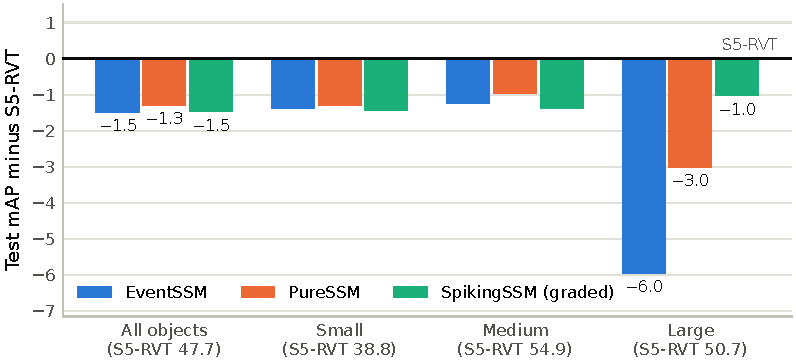
\includegraphics[width=\textwidth]{images/fig_accuracy_by_size.pdf}
    \caption[Test accuracy by object size relative to S5-RVT]{Gen1 test AP of the own 400k-step models minus that of S5-RVT, over all objects and by object size
    (COCO mAP@[0.50:0.95]); S5-RVT's own AP is given under each group. The three models are within 0.5 of each
    other on small and medium objects; on large objects PureSSM's gap ($-3.0$) is half of EventSSM's ($-6.0$), and
    the graded SpikingSSM's ($-1.0$) is the smallest (Section~\ref{subsec:spk_full}).}
    \label{fig:acc_by_size}
\end{figure}

\section{Effective Receptive Field}
\label{sec:erf}
\guide{100}{
  \item What the probe measures: gradient of the centre feature with respect to the input~\cite{luo2016understanding}, averaged over 8 random inputs; $\sigma$ = RMS spread in pixels.
  \item Table~\ref{tab:erf}: BiMamba 85.6/105.5\,px vs ResNet 41.8/84.4\,px at stages 3/4; training widened BiMamba by 30--34\,px, ResNet by 0.2/6.2\,px.
}
To explain the large-object result, a gradient-based probe~\cite{luo2016understanding} measured how much of
the input each trained spatial mixer actually uses: the gradient magnitude of the feature at the frame
centre with respect to the input, averaged over eight random inputs, with $\sigma$ the root-mean-square
spread of that gradient in input pixels. Table~\ref{tab:erf} and Figure~\ref{fig:erf} give the result. The
state-space mixer sees wider at both measured stages, 85.6 against 41.8~px at stage~3 and 105.5 against
84.4~px at stage~4, and training widened its field by 30--34~px, against 0.2 and 6.2~px for the
convolutional stack.

\begin{table}[htbp]
\centering
\caption[Effective receptive field extent by stage]{Trained effective receptive field, and the change induced by training, measured against a
random initialisation of the same architecture.}
\label{tab:erf}
\begin{tabular}{lccc}
\toprule
\textbf{Backbone} & \textbf{Stage 3 $\sigma$} & \textbf{Stage 4 $\sigma$} & \textbf{$\Delta$ from training} \\
\midrule
ResNet-18 (EventSSM) & 41.8\,px & 84.4\,px & $+0.2$ / $+6.2$ \\
BiMamba (PureSSM)    & \textbf{85.6\,px} & \textbf{105.5\,px} & $\mathbf{+34.4}$ / $\mathbf{+30.1}$ \\
\bottomrule
\end{tabular}
\end{table}

\guide{150}{
  \item Why: a convolutional field is set by kernel size and depth (approximately Gaussian, grows with $\sqrt{\text{depth}}$), so training barely moves it.
  \item In a scan every token can reach every other; the reach is set by learned decays and steps (Equation~\eqref{eq:mamba2_state}) $\Rightarrow$ a learned quantity.
  \item Untrained, BiMamba is not wider at stage 4 (75.4 vs 78.2\,px): the advantage is acquired in training.
  \item Caveats: random inputs, not events; ResNet reference is a random init, not ImageNet.
}
The difference has a structural explanation. In a convolutional stack the effective receptive field is
governed by kernel size and depth; it is approximately Gaussian and grows only with the square root of
the number of layers~\cite{luo2016understanding}, so training reshapes it little. In a scan, every token
can influence every other through the forward and backward passes, and how far that influence reaches is
set by the learned decays and steps of Equation~\eqref{eq:mamba2_state}, which training can lengthen. The
reach of the state-space mixer is therefore learned, while that of the convolutional stack is largely
fixed by its architecture. Notably, the untrained BiMamba field is no wider than the ResNet's at stage~4
(75.4 against 78.2~px): the advantage is acquired in training. Two caveats apply: the probe uses random
inputs rather than events, and the untrained ResNet reference is a random initialisation rather than the
ImageNet weights EventSSM started from.

\begin{figure}[htbp]
    \centering
    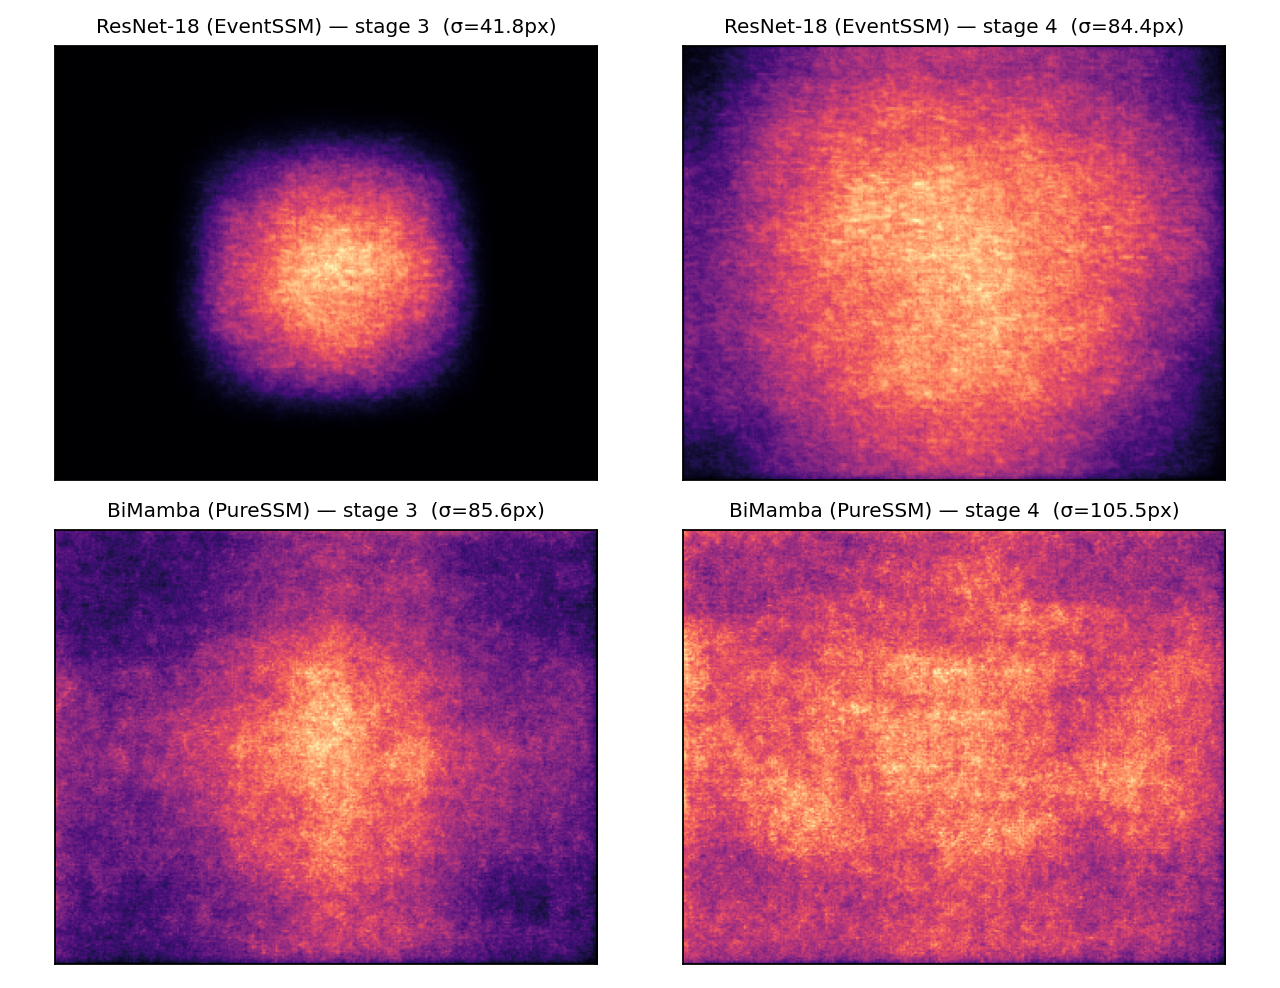
\includegraphics[width=0.85\textwidth]{images/fig_erf_trained.png}
    \caption[Effective receptive fields of the trained backbones]{Effective receptive field of the trained spatial backbones at the frame centre, stages 3
    and 4: gradient magnitude of the centre feature with respect to the input (log colour scale, averaged
    over 8 random inputs). $\sigma$ is the RMS spatial spread in input pixels. The BiMamba field is wider
    at both stages and less concentrated on the centre.}
    \label{fig:erf}
\end{figure}

\section{Temporal Robustness}
\label{sec:robustness}
\guide{20}{
  \item The two regimes of Section~\ref{subsec:eval_rob}, then the $\Delta t$ reproduction.
}
This section reports the two regimes of Section~\ref{subsec:eval_rob} and then the attempt to reproduce
the inference-time $\Delta t$ compensation.

\subsection{Fixed Cadence, Variable Accumulation Window}
\guide{110}{
  \item Table~\ref{tab:regime1}: own models tied across the sweep, marginally below the baseline.
  \item At $0.25\times$ (200\,ms) PureSSM leads overall (41.65 vs 40.95) because of large objects: the baseline's $\mathrm{AP}_L$ falls 14.3, PureSSM's 7.7.
  \item Conclusion: PureSSM more robust at the dense, slow end; the baseline at the sparse, fast end.
}
With the cadence fixed at 50~ms, the two own models are tied across the window sweep and both lie
marginally below the baseline (Table~\ref{tab:regime1}). One result at the dense end needs care. With
200-ms windows ($0.25\times$), PureSSM exceeds the baseline overall (41.65 against 40.95), and the margin
comes from large objects: on the smeared, dense frames the baseline's $\mathrm{AP}_L$ falls by 14.3 points
and PureSSM's by 7.7. The overall margin is too small to separate with single runs; the large-object
difference is the larger effect. PureSSM is therefore the more robust model at the dense, slow end of the
sweep, and the baseline at the sparse, fast end.

\begin{table}[htbp]
\centering
\caption[Robustness at a fixed cadence with a varied window]{Accumulation-window sweep (COCO mAP $\times$ 100). Training operating point is $1\times$.
PureSSM is given to two decimals; its $1\times$ value (46.45) is measured on the re-preprocessed test set
used for the sweep and differs from the canonical 46.43 only through that preprocessing.}
\label{tab:regime1}
\begin{tabular}{llccc}
\toprule
\textbf{Multiplier} & \textbf{$\Delta t$} & \textbf{S5-RVT} & \textbf{EventSSM} & \textbf{PureSSM} \\
\midrule
$0.25\times$ & 200\,ms & 41.0 & 40.9 & \textbf{41.65} \\
$0.5\times$  & 100\,ms & 46.5 & 45.5 & 45.67 \\
$1\times$    & 50\,ms  & 47.7 & 46.2 & 46.45 \\
$2\times$    & 25\,ms  & 45.0 & 43.5 & 44.09 \\
$4\times$    & 12.5\,ms & 38.4 & 35.4 & 35.68 \\
\bottomrule
\end{tabular}
\end{table}

\subsection{True Event-Rate Change}
\guide{90}{
  \item Table~\ref{tab:regime2}: at a true $10\times$ rate, retention 62.2\,\% (S5-RVT), 63.0\,\% (EventSSM), 69.7\,\% (PureSSM); at $2\times$ all keep about 95\,\%.
  \item The ConvLSTM baseline under the same protocol: \res{measured retention} (1$\times$: 47.14).
  \item The temporal path of EventSSM and PureSSM is identical $\Rightarrow$ the extra robustness comes from the spatial backbone; the wider field is plausible but untested.
}
Under a true change of rate the models separate (Table~\ref{tab:regime2}, Figure~\ref{fig:robustness}).
At twice the rate all three keep about 95\,\% of their accuracy. At ten times the rate, with 5-ms windows
at 200\,Hz and no retraining, S5-RVT and EventSSM retain 62.2 and 63.0\,\% and PureSSM 69.7\,\%, the most
of the models tested. RVT's ConvLSTM, measured under the same protocol from its 47.14~mAP at the training
rate, retains \res{\%}. Because EventSSM and PureSSM share an identical temporal path, PureSSM's additional
robustness must originate in its spatial backbone. The wider receptive field is a plausible explanation,
since frames at ten times the rate carry few events, but it has not been tested directly.

\begin{table}[htbp]
\centering
\caption[Robustness under a true event-rate change]{True event-rate change. Retention $=\mathrm{mAP}@\text{rate} \div \mathrm{mAP}@1\times$.
$^{\dagger}$Published by Zubic et al.~\cite{zubic2024state} for RVT at 200\,Hz, obtained with
preprocessing that was not released; not measured on this test set (Section~\ref{subsec:f2}).}
\label{tab:regime2}
\begin{tabular}{lcccc}
\toprule
 & \textbf{S5-RVT} & \textbf{EventSSM} & \textbf{ConvLSTM}$^{\dagger}$ & \textbf{PureSSM} \\
\midrule
true-$10\times$ mAP        & 29.67 & 29.09 & 8.35 & \textbf{32.38} \\
true-$10\times$ retention  & 62.2\% & 63.0\% & 17.7\% & \textbf{69.7\%} \\
true-$2\times$ retention   & 95.1\% & 95.5\% & --- & \textbf{95.9\%} \\
\bottomrule
\end{tabular}
\end{table}

\begin{figure}[htbp]
    \centering
    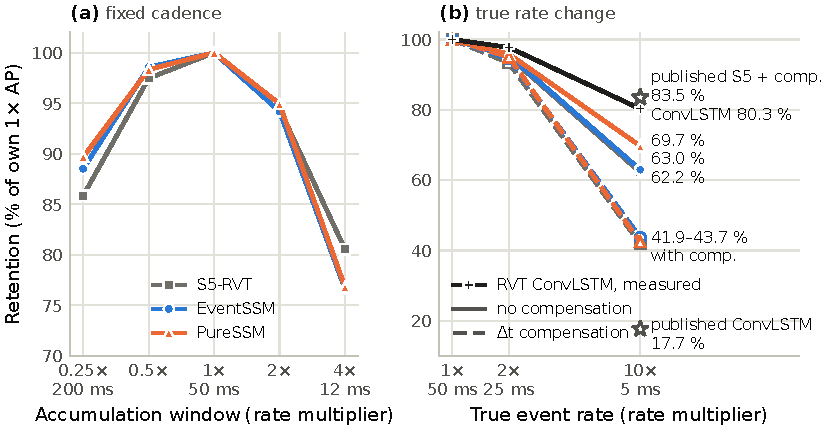
\includegraphics[width=\textwidth]{images/fig_robustness.pdf}
    \caption[Temporal robustness under event-rate change]{Temporal robustness as retention, the mAP at each operating point as a percentage of the model's
    own $1\times$ mAP. (a) Fixed 50-ms cadence with a shortened or lengthened accumulation window
    (Table~\ref{tab:regime1}). (b) True event-rate change (Tables~\ref{tab:regime2} and~\ref{tab:dt_comp}):
    solid lines without and dashed lines with inference-time $\Delta t$ compensation; stars are published
    values not measured on this test set, S5 with compensation at 200\,Hz (83.5\,\%) and RVT's ConvLSTM
    (17.7\,\%)~\cite{zubic2024state}.}
    \label{fig:robustness}
\end{figure}

\subsection{Reproducing Inference-Time \texorpdfstring{$\Delta t$}{Delta t}-Rescaling}
\label{subsec:f2}
\guide{170}{
  \item The published claim: rescaling the step at inference gives S5 39.84 at 200\,Hz.
  \item Table~\ref{tab:dt_comp}: compensation lowered accuracy at every tested point, by 9--13\,mAP at $10\times$, for S5 and both Mamba models.
  \item The published 39.84 could not be reproduced (best 29.67, uncompensated); the released preprocessing cannot produce a true-rate test set (stride fixed at 50\,ms).
  \item The robustness itself is reproduced without compensation. Soft wording only: ``not reproducible under the published artefacts''.
}
Zubi\'{c} et al.~\cite{zubic2024state} report that state-space detectors generalise to unseen event rates
when the discretisation step is rescaled at inference, giving 39.84~mAP at 200\,Hz for S5 with this
compensation. This work attempted to reproduce that result with the published checkpoint and code, and
transferred the compensation to Mamba by rescaling its step $\Delta_t$ by the same factor
(Table~\ref{tab:dt_comp}). Under the published artefacts the compensation did not recover accuracy at any
tested operating point: at ten times the rate it lowered mAP by 9.7, 8.9 and 12.7 points for S5-RVT,
EventSSM and PureSSM. The published 200\,Hz figure could not be reproduced; the best S5 result at a true
tenfold rate is 29.67, without compensation. The released preprocessing also cannot produce a true-rate
test set, because its frame stride is fixed at 50~ms, so the published experiment must have used
preprocessing that was not released, which may account for the difference. The rate robustness itself is
reproduced: without any compensation, every state-space model keeps 62--70\,\% of its accuracy.

\begin{table}[htbp]
\centering
\caption[Effect of inference-time \texorpdfstring{$\Delta t$}{Delta t} compensation]{Inference-time $\Delta t$ compensation under a true rate change (regime~2), mAP on the Gen1
test split. ``Comp.'' rescales the step by the window ratio, the convention of~\cite{zubic2024state}.
The published reference is S5 with compensation at 200\,Hz.}
\label{tab:dt_comp}
\begin{tabular}{llcccc}
\toprule
True rate & & \textbf{S5-RVT} & \textbf{EventSSM} & \textbf{PureSSM} & Published \\
\midrule
$2\times$ (25\,ms)  & no comp.  & 45.37 & 44.13 & 44.53 & --- \\
                    & comp.     & 44.51 & 43.67 & 44.13 & --- \\
\midrule
$10\times$ (5\,ms)  & no comp.  & \textbf{29.67} & \textbf{29.09} & \textbf{32.38} & --- \\
                    & comp.     & 19.96 & 20.18 & 19.70 & 39.84 \\
                    & difference & $-9.71$ & $-8.91$ & $-12.68$ & \\
\bottomrule
\end{tabular}
\end{table}

\section{Efficiency}
\label{sec:efficiency}
\guide{110}{
  \item Table~\ref{tab:efficiency}: PureSSM fewest parameters (16.33\,M) and FLOPs (10.03\,G), best mAP/GFLOP (4.63).
  \item But slowest in eager execution (26.86\,ms, 37\,Hz): many small scan kernels, launch-bound; CUDA graphs lift it to 181\,Hz; EventSSM fastest in both modes (79 / 210\,Hz) and lowest energy (0.438\,J).
}
Table~\ref{tab:efficiency} and Figure~\ref{fig:efficiency} show that efficiency is a trade-space rather than
a ranking. PureSSM has the fewest parameters (16.33\,M) and FLOPs (10.03\,G) and the best accuracy per
GFLOP (4.63), yet it is the slowest model in eager execution, at 26.86~ms per frame (37\,Hz). Its backbone
consists of many small scan operations, so it is bound by kernel-launch overhead rather than by
arithmetic. CUDA-graph replay removes most of that overhead and lifts it to 181\,Hz, the largest speed-up
of any model, but EventSSM stays ahead in both modes (79 and 210\,Hz) and draws the least energy per frame
(0.438~J against 0.723~J for the baseline).

\begin{table}[htbp]
\centering
\caption[Efficiency of the non-spiking models]{Full-pipeline streaming inference, RTX 5070 Ti, idle-GPU-guarded harness. FLOPs per frame
are counted as defined in Section~\ref{sec:eval_protocol}; mAP per GFLOP uses the test AP of
Table~\ref{tab:accuracy}.}
\label{tab:efficiency}
\begin{tabular}{lccc}
\toprule
\textbf{Metric} & \textbf{S5-RVT} & \textbf{EventSSM} & \textbf{PureSSM} \\
\midrule
Total parameters       & 18.19\,M & 19.18\,M & \textbf{16.33\,M} \\
FLOPs                  & 11.06\,G & 12.71\,G & \textbf{10.03\,G} \\
mAP per GFLOP          & 4.32 & 3.64 & \textbf{4.63} \\
Latency p50, eager     & 17.14\,ms & \textbf{12.60\,ms} & 26.86\,ms \\
Throughput, eager      & 58\,Hz & \textbf{79\,Hz} & 37\,Hz \\
Throughput, CUDA-graph & --- & \textbf{210\,Hz} & 181\,Hz \\
Energy per frame       & 0.723\,J & \textbf{0.438\,J} & 0.652\,J \\
Streaming state        & \textbf{4.7\,MB} & 144\,MB & 144\,MB \\
\bottomrule
\end{tabular}
\end{table}

\guide{80}{
  \item Event sparsity does not translate into GPU speed: every frame is processed densely.
  \item Streaming state: 144\,MB for both Mamba models vs 4.7\,MB for the baseline (31$\times$, Mamba's state expansion at every location) --- the number to watch on a memory-limited platform.
}
Two further results qualify the picture. Event sparsity does not translate into speed on a GPU, because
every frame is processed densely whatever its event count; the efficiency claim for the state-space
models is therefore about computation and robustness, not about sparse inputs being fast. And the Mamba
models carry a streaming state of 144~MB per stream, 31 times the baseline's 4.7~MB, because Mamba expands
its state at every spatial location; on a memory-constrained platform this is the number to watch.

\begin{figure}[htbp]
    \centering
    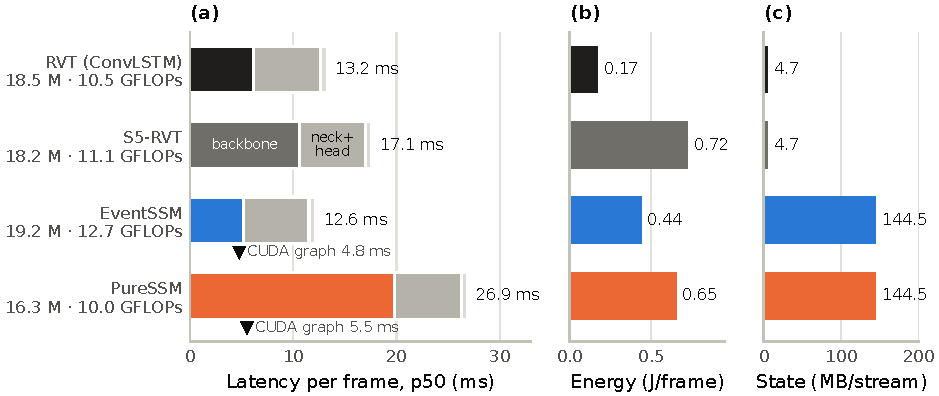
\includegraphics[width=\textwidth]{images/fig_efficiency.pdf}
    \caption[Efficiency of the non-spiking models]{Efficiency of the three non-spiking models (values of Table~\ref{tab:efficiency}; parameters and
    GFLOPs per frame in the row labels). (a) Eager p50 latency per frame, split into backbone, neck and head,
    and post-processing; the marker is the latency with CUDA-graph replay of the network plus eager
    post-processing. (b) Measured GPU energy per frame. (c) Streaming state carried per stream.}
    \label{fig:efficiency}
\end{figure}

\section{Qualitative Results}
\label{sec:qualitative}
\guide{150}{
  \item How the recording was chosen (most large-car instances; 8 evenly spaced frames, not hand-picked).
  \item Observations: close moving cars detected confidently (0.81--0.93); detections persist when events vanish (state carries the object); low-confidence false boxes at the start (empty state); ground truth flickers and misses pedestrians.
  \item The two models look alike, as expected from their identical temporal path; the difference rests on the quantitative $\mathrm{AP}_L$.
}
Figure~\ref{fig:qualitative} shows the test recording with the most large-car instances, as eight evenly
spaced frames that were not selected by hand. Four behaviours recur across the recordings inspected.
Close cars that generate events are detected with high confidence (0.81--0.93). Detections persist when
the scene goes quiet: when almost no events fall on a car, both models keep it at 0.70--0.90 confidence,
because the object is carried by the recurrent state rather than seen in the current frame. At the start
of a recording, with an empty state and few events, both models emit low-confidence boxes where there is
no object. And the ground truth itself flickers and misses visible pedestrians, so a correct detection can
count as a false positive. The two models behave very similarly on these frames, as expected from their
identical temporal path; the difference between them rests on the quantitative result of
Section~\ref{sec:acc_results}.

\begin{figure}[htbp]
    \centering
    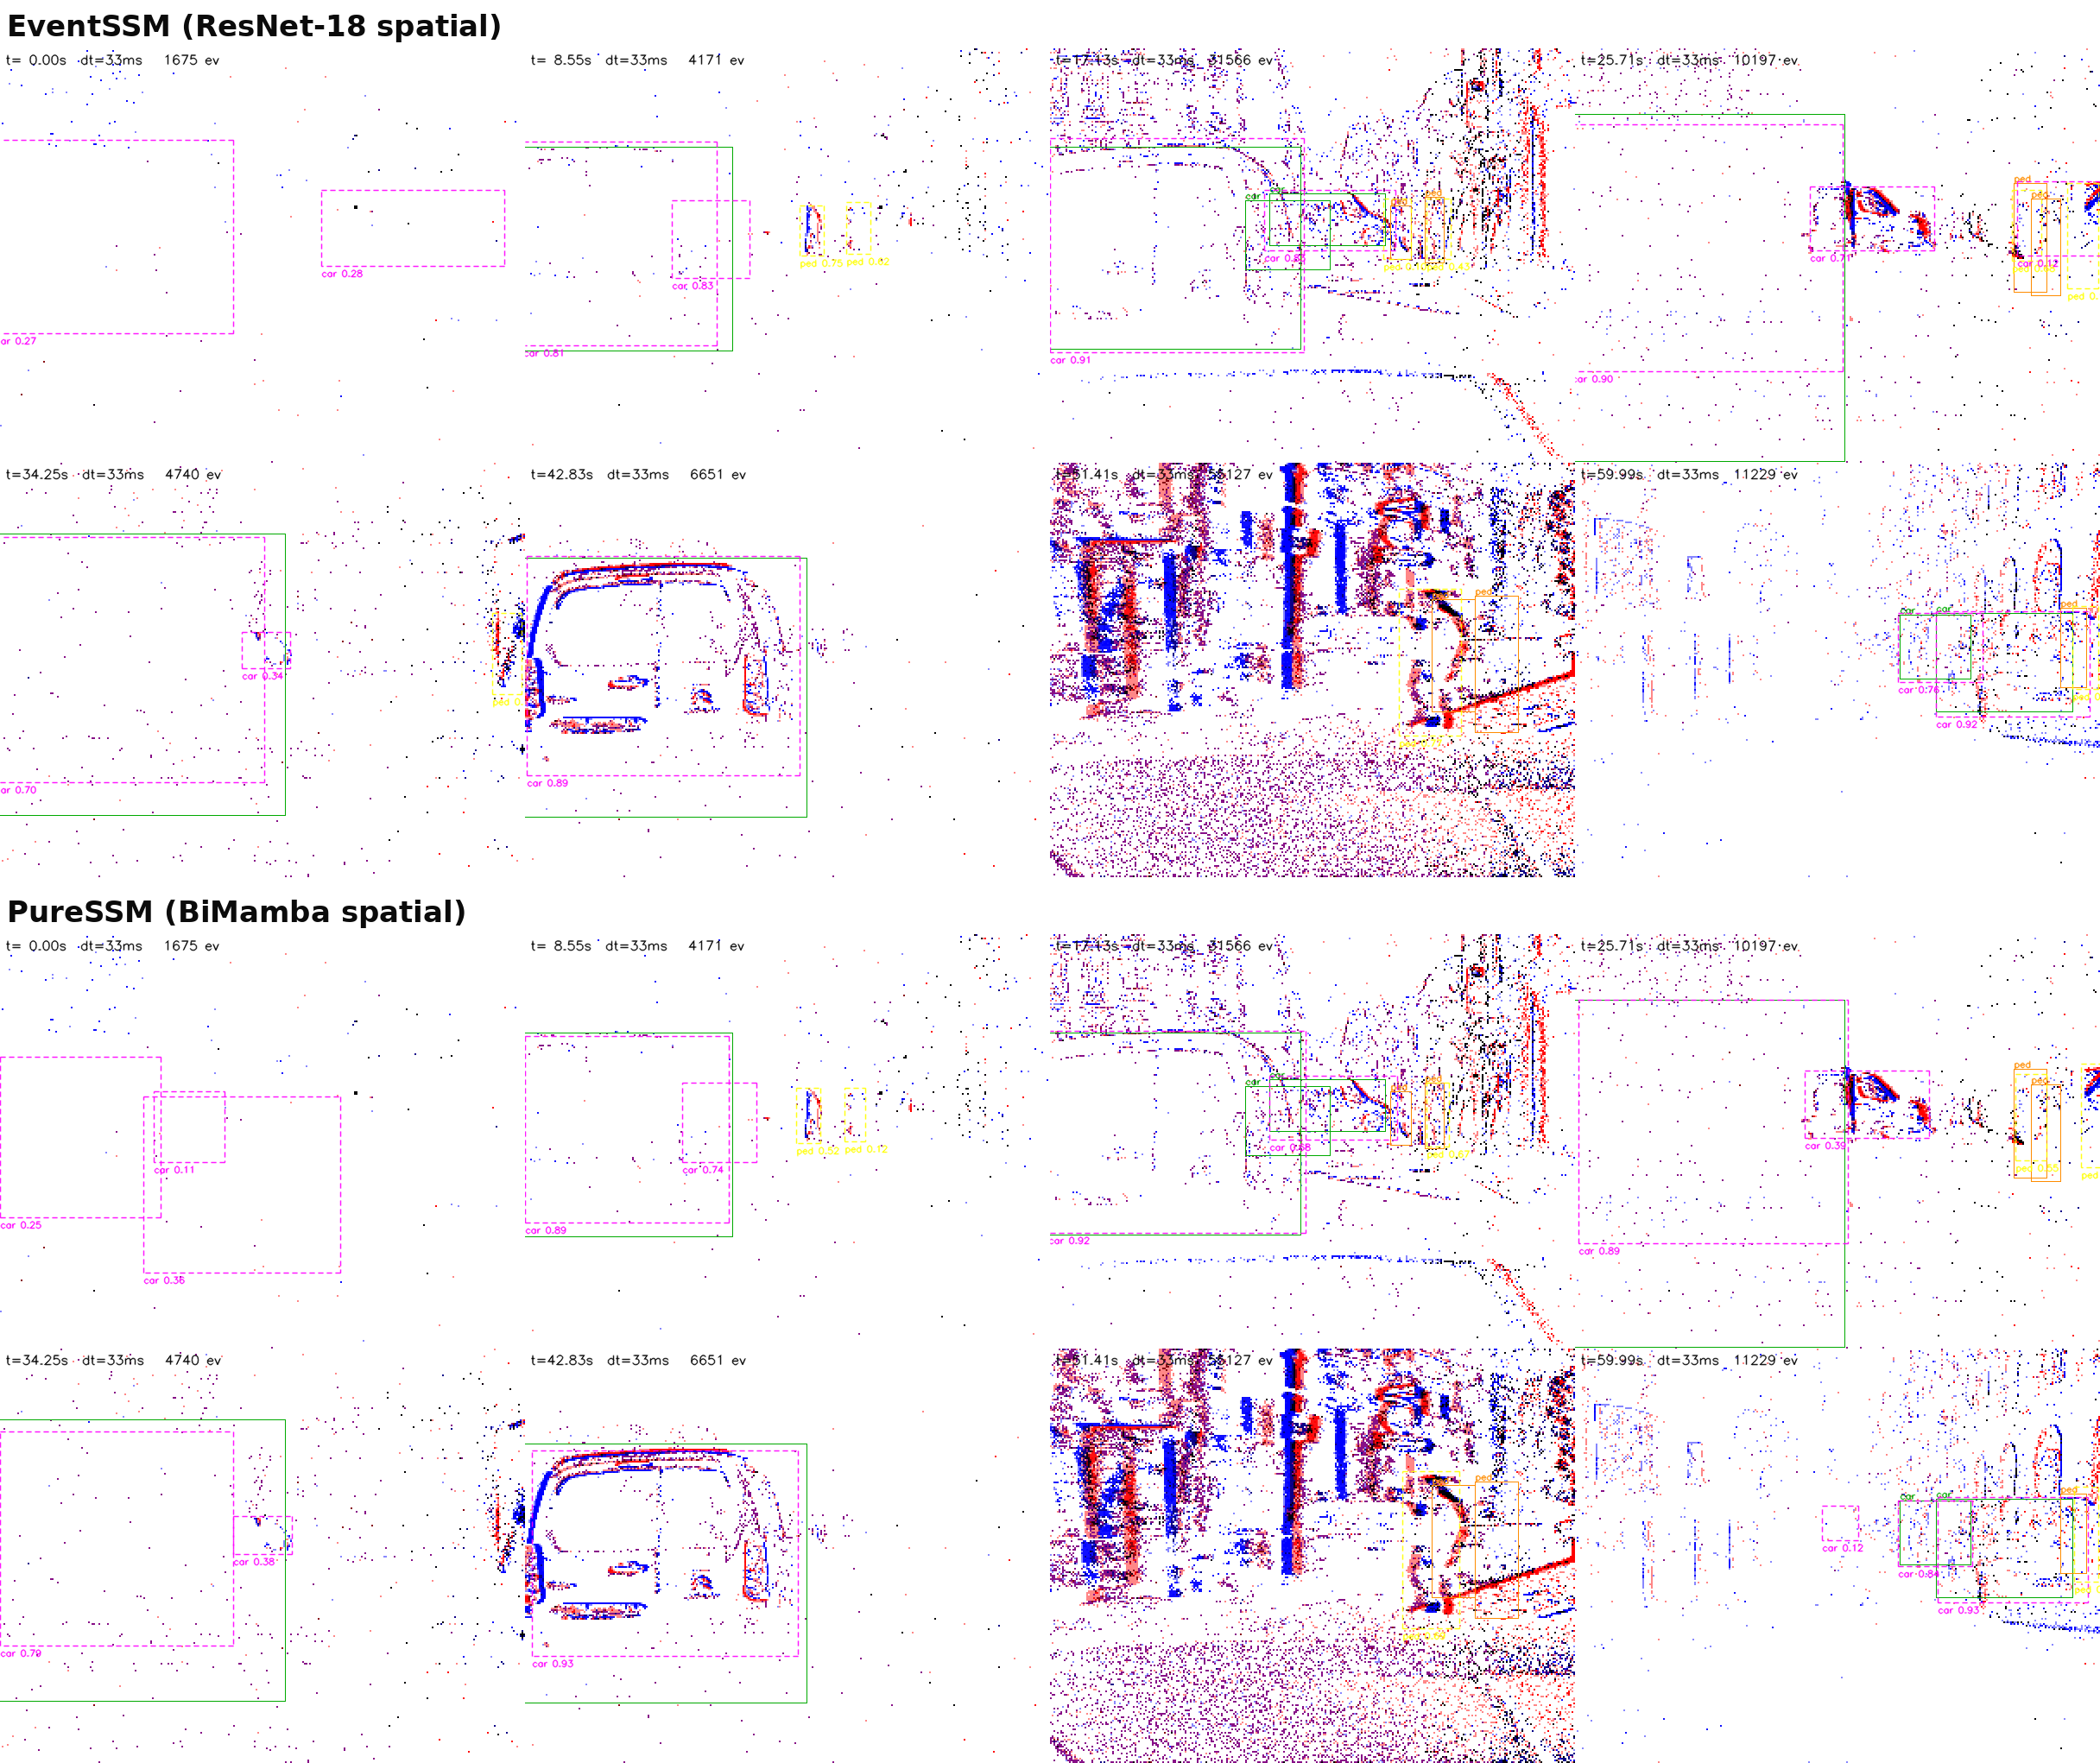
\includegraphics[width=\textwidth]{images/fig_qualitative_large_car.png}
    \caption[Ground truth and predictions on a large-car recording]{Ground truth against predictions on the test recording with the most large-car instances
    (\texttt{18-03-29\_13-15-02\_500000\_60500000}), eight evenly spaced frames from its 60~s; top
    EventSSM, bottom PureSSM. Events of 33~ms are drawn by polarity (red/blue). Solid boxes are ground
    truth (car green, pedestrian orange), each held for up to 250~ms after its annotation; dashed boxes
    are predictions with their confidence (car magenta, pedestrian yellow), shown down to RVT's
    default inference threshold of 0.1 (the AP evaluation itself uses 0.001).}
    \label{fig:qualitative}
\end{figure}

\section{Spiking SSM Detector}
\label{sec:spiking_results}
\guide{90}{
  \item The model is a hybrid (only the temporal readout spikes), so it is not a like-for-like competitor to fully spiking detectors (Table~\ref{tab:snn_landscape}).
  \item The result is the decomposition of the cost of spiking; the ladder is on the 100k-step schedule against a PureSSM trained on the same schedule; graded also on the full 400k schedule.
}
The spiking model is a hybrid: only its temporal readout spikes, and its spatial backbone is PureSSM's. It is
therefore not a like-for-like competitor to the fully spiking detectors of Table~\ref{tab:snn_landscape},
and its accuracy is context rather than a position in that landscape. The result of this section is the
decomposition of what spiking costs. The three readouts were trained on the 100k-step schedule and are
compared with a PureSSM trained on the same schedule; the graded readout was also trained on the full
400k-step schedule (Section~\ref{subsec:spk_full}).

\subsection{Accuracy of the Readouts}
\label{subsec:spk_accuracy}
\guide{80}{
  \item Table~\ref{tab:spiking_ablation}: PureSSM 42.52, analog 42.25, graded 40.72, spike 40.18 (100k steps); total cost of spiking 2.34.
  \item The cost falls mainly on pedestrians (car $-1.61$, pedestrian $-3.07$).
  \item Per-arm intervals about 4 points wide and overlapping; the paired steps are what is tested (next subsection).
}
On the 100k-step schedule, the four arms reach 42.52 (PureSSM), 42.25 (analog), 40.72 (graded) and 40.18
(binary) test mAP (Table~\ref{tab:spiking_ablation}), so making the readout binary costs 2.34 points in
total. The cost falls mainly on pedestrians: from PureSSM to the binary readout, car AP drops by 1.61 and
pedestrian AP by 3.07. The per-arm intervals are about 4~points wide and overlap, because each carries the
difficulty of the particular test recordings; the comparison between arms is therefore made on paired
differences.

\begin{table}[htbp]
\centering
\caption[Accuracy of the spiking readouts (100k steps)]{Spiking readouts on Gen1 (test set, 100k-step schedule, spiking stages 2--4). Intervals: 95\,\%
paired bootstrap over the 470 test recordings. Firing rate: share of nonzero readout outputs, weighted by the
neck operations each stage feeds, on the final checkpoint.}
\label{tab:spiking_ablation}
\begin{tabular}{lccccc}
\toprule
\textbf{Model (100k steps)} & \textbf{mAP [95\,\% CI]} & \textbf{AP\textsubscript{50}} & \textbf{AP\textsubscript{L}} & \textbf{Car / Ped.} & \textbf{Firing rate} \\
\midrule
PureSSM (no LIF)   & 42.52 [40.40, 44.39] & 69.40 & 42.62 & 60.43 / 24.62 & n/a \\
analog (dense LIF) & 42.25 [40.14, 43.99] & 69.55 & 42.41 & 59.72 / 24.77 & 1.00 (dense) \\
graded             & 40.72 [38.66, 42.33] & 67.57 & 38.41 & 59.09 / 22.36 & 0.17 \\
spike (binary)     & 40.18 [38.09, 41.88] & 66.40 & 41.14 & 58.82 / 21.55 & 0.41 \\
\bottomrule
\end{tabular}
\end{table}

\subsection{The Readout Ladder}
\label{subsec:spk_ladder}
\guide{100}{
  \item The three steps with intervals: dynamics $-0.28$ $[-0.63, 0.05]$, sparsity $-1.52$ $[-1.98, -1.06]$, binarisation $-0.54$ $[-1.07, -0.07]$.
  \item H3 held, in the point estimates and the intervals; the dynamics step is not distinguishable from zero.
  \item Sparsity is the largest step (about 3$\times$ binarisation); paired intervals 4--6$\times$ narrower than per-arm ones.
}
The steps of the ladder (Equation~\eqref{eq:ladder}, Figure~\ref{fig:spiking_ladder}) measured
$\Delta_{\mathrm{dyn}} = -0.28$ $[-0.63, 0.05]$, $\Delta_{\mathrm{sparse}} = -1.52$ $[-1.98, -1.06]$ and
$\Delta_{\mathrm{bin}} = -0.54$ $[-1.07, -0.07]$~mAP. The pre-registered ordering analog $\geq$ graded $>$
binary held, in the point estimates and in the intervals: the sparsity and binarisation steps exclude
zero, while the dynamics step does not, so the cost of the leak and reset is not distinguishable from zero
on Gen1. The largest step is sparsity, about three times the cost of binarisation. Because every arm is
scored on the same resampled recordings, the step intervals are four to six times narrower than the
per-arm intervals.

\begin{figure}[htbp]
\centering
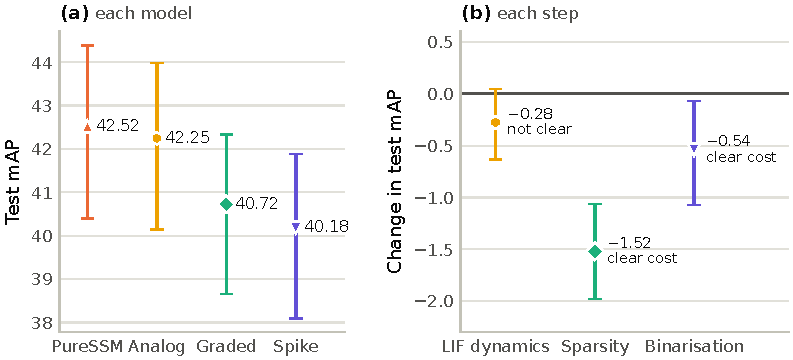
\includegraphics[width=\textwidth]{images/fig_ladder.pdf}
\caption[The cost of spiking, step by step]{The cost of spiking, step by step (100k-step schedule, Gen1 test set). (a) Test mAP per arm. (b) The
paired change at each step of the ladder: LIF dynamics (PureSSM $\rightarrow$ analog), sparsity (analog
$\rightarrow$ graded) and binarisation (graded $\rightarrow$ spike). Whiskers are 95\,\% bootstrap intervals
over the 470 test recordings; the paired intervals in (b) are narrower than the per-arm intervals in (a)
because every arm is scored on the same resampled recordings.}
\label{fig:spiking_ladder}
\end{figure}

\guide{110}{
  \item By object size: sparsity costs on small ($-1.88$) and medium ($-1.23$) objects; binarisation on medium ($-1.06$) but not small ($-0.06$); large-object intervals too wide (6--8 points) for any claim.
  \item Validation curves (Figure~\ref{fig:training_curves}): graded ahead of binary only from 60k steps (binary led at 10--30k and 50k); analog within 1.8 points of the anchor throughout; the binarisation gap shrank from 3.5 (25k pilot) to 0.7 at 100k.
}
By object size, sparsity costs on small ($-1.88$ $[-2.24, -1.44]$) and medium objects ($-1.23$
$[-1.91, -0.53]$), whereas binarisation costs on medium objects ($-1.06$ $[-1.87, -0.37]$) but not on small
ones ($-0.06$ $[-0.63, 0.32]$); the large-object intervals of every step are 6 to 8 points wide, so no step
is credited with a large-object effect. On the validation split the full ordering emerged only late in
training (Figure~\ref{fig:training_curves}): the binary readout was ahead of the graded one at 10--30k and
50k steps, and behind it from 60k steps on, while the analog readout stayed within 1.8 points of the
anchor throughout. The binarisation gap narrowed accordingly, from 3.5 points in a 25k-step pilot to 0.7
at 100k.

\begin{figure}[htbp]
    \centering
    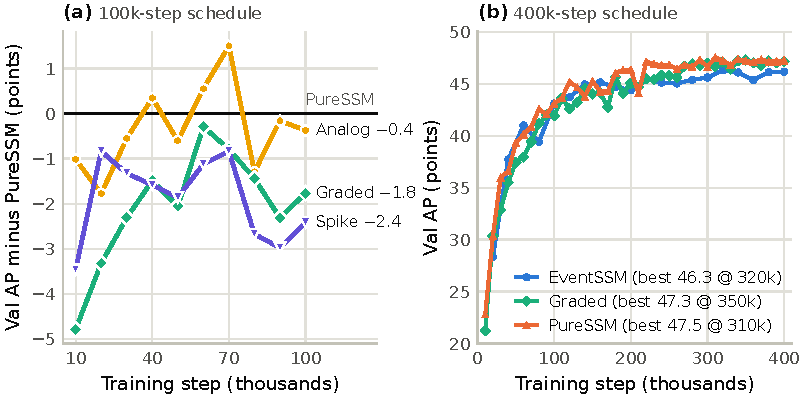
\includegraphics[width=\textwidth]{images/fig_training_curves.pdf}
    \caption[Validation mAP during training]{Validation mAP during training. (a) The three 100k-step readouts minus the PureSSM anchor trained
    on the same schedule, at every 10k-step validation; end labels are the final differences. (b) The
    400k-step runs of EventSSM, PureSSM and the graded readout (PureSSM trained on a rented RTX~5090, the
    others on the local RTX~5070~Ti; the schedule is identical).}
    \label{fig:training_curves}
\end{figure}

\subsection{The Graded Readout on the Full Schedule}
\label{subsec:spk_full}
\guide{120}{
  \item Trained for 400k steps with the full recipe (resumed three times); best checkpoint 350k (validation 47.28).
  \item Table~\ref{tab:spiking_400k}: 46.24, 0.19 below PureSSM (\res{paired interval}) and level with EventSSM; at 100k it was 1.80 below its anchor $\Rightarrow$ the cost at 100k is mostly slower convergence.
  \item $\mathrm{AP}_L$ 49.63: highest of the proposed models (+1.98 over PureSSM, \res{interval}), 1.03 below S5-RVT.
}
Trained for 400k steps with the same recipe as the other full-schedule models, the graded readout reaches
46.24~mAP, 0.19 below PureSSM (paired interval \res{[lo, hi]}) and level with EventSSM
(Table~\ref{tab:spiking_400k}). At 100k steps the same readout was 1.80 below its PureSSM anchor, so most of
its short-schedule cost is slower convergence rather than lost capacity. Its large-object AP of 49.63 is the
highest of the proposed models, 1.98 above PureSSM (\res{[lo, hi]}) and 1.03 below S5-RVT. Validation
mAP was flat between 46.8 and 47.3 from 350k steps on, and the best checkpoint (350k, validation 47.28) is
the one evaluated; the run was resumed three times, which changes its data order but not its schedule.

\begin{table}[htbp]
\centering
\caption[The graded readout on the full schedule]{The graded readout trained on the full 400k-step schedule, against the 400k-step models of
Table~\ref{tab:accuracy} (Gen1 test set, best-validation checkpoint of each run). Single runs; the paired
interval of the graded--PureSSM difference is \res{[lo, hi]}.}
\label{tab:spiking_400k}
\begin{tabular}{lcccc}
\toprule
\textbf{Metric} & \textbf{S5-RVT} & \textbf{EventSSM} & \textbf{PureSSM} & \textbf{SpikingSSM, graded} \\
\midrule
mAP @[0.50:0.95]        & 47.72 & 46.22 & 46.43 & 46.24 \\
$\mathrm{AP}_{50}$      & 75.28 & 74.54 & 74.09 & 73.86 \\
$\mathrm{AP}_{75}$      & 49.76 & 48.08 & 48.25 & 48.42 \\
$\mathrm{AP}_S$ (small) & 38.81 & 37.42 & 37.50 & 37.38 \\
$\mathrm{AP}_M$ (medium)& 54.92 & 53.68 & 53.96 & 53.54 \\
$\mathrm{AP}_L$ (large) & 50.66 & 44.70 & 47.65 & 49.63 \\
\midrule
Car / Pedestrian        & 63.88 / 31.56 & 61.67 / 30.78 & 62.83 / 30.02 & 61.93 / 30.54 \\
Checkpoint (step)       & published & 320k & 310k & 350k \\
\bottomrule
\end{tabular}
\end{table}

\guide{80}{
  \item Figure~\ref{fig:training_400k}: the loss curves of the three 400k runs overlap within noise; no instability after the resumes.
  \item Figure~\ref{fig:training_400k_time}: 55.5\,h for the graded run vs 27.9\,h for EventSSM on the same GPU (activation recomputation in BiMamba + the per-step LIF loop); PureSSM's run was on another GPU.
}
The training curves of the three full-schedule runs (Figure~\ref{fig:training_400k}) overlap within their
noise throughout, with no instability after any of the resumes. Training is slower, however
(Figure~\ref{fig:training_400k_time}): the graded run took 55.5~h on the RTX~5070~Ti against 27.9~h for
EventSSM on the same GPU, because the BiMamba blocks are trained with activation recomputation and the LIF
readout adds a loop over time steps. PureSSM's run was made on a different GPU and is not timed against
these.

\begin{figure}[htbp]
    \centering
    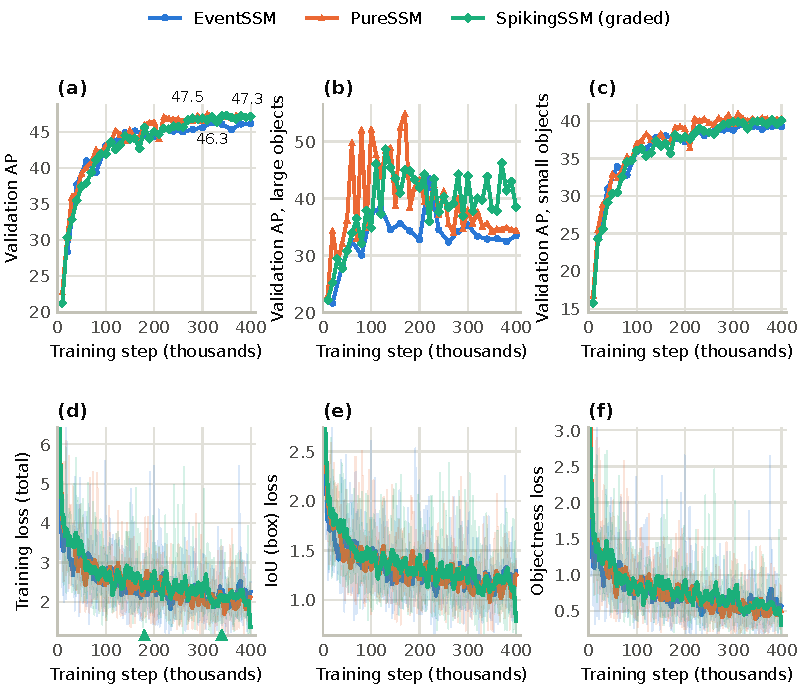
\includegraphics[width=\textwidth]{images/fig_training_400k.pdf}
    \caption[Validation accuracy and training losses of the 400k-step runs]{The 400k-step runs of EventSSM, PureSSM and the graded readout against training step: validation (a) mAP,
    (b) large-object and (c) small-object AP; training (d) total, (e) IoU and (f) objectness loss, raw (faint)
    and smoothed. Triangles in (d) mark the steps from which the graded run was resumed (180k and 340k).}
    \label{fig:training_400k}
\end{figure}

\begin{figure}[htbp]
    \centering
    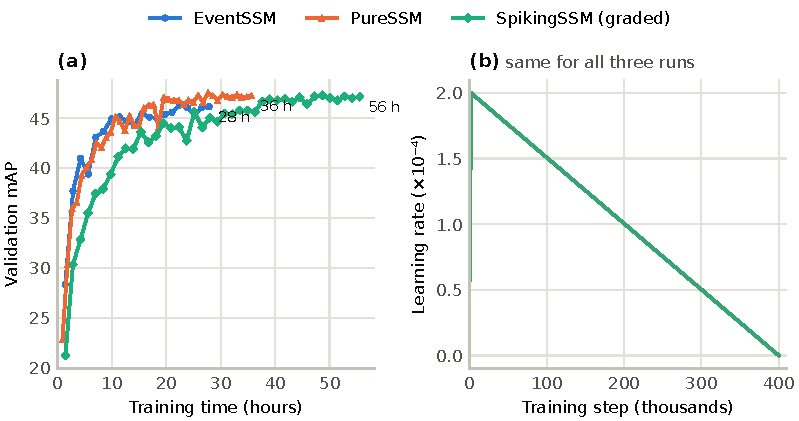
\includegraphics[width=\textwidth]{images/fig_training_400k_time.pdf}
    \caption[Validation mAP against wall-clock time]{(a) Validation mAP of the same three runs against training wall-clock time; EventSSM and the graded
    readout trained on the local RTX~5070~Ti, PureSSM on a rented RTX~5090, so its hours are not directly comparable.
    The steps repeated after each resume are excluded. (b) The learning-rate schedule (OneCycle over 400k steps),
    identical for all three runs.}
    \label{fig:training_400k_time}
\end{figure}

\subsection{Firing Activity and the Threshold Trade-off}
\label{subsec:spk_firing}
\guide{130}{
  \item Firing rates on a test recording: graded 0.28/0.12/0.10, binary 0.48/0.36/0.39 (stages 2/3/4); binary rates roughly doubled during training, graded rates at stages 3--4 fell (Figure~\ref{fig:spiking_firing}).
  \item The binary readout appears to compensate for its one-bit output by firing more.
  \item Sparsity is structural, not event-driven: only graded stage 2 follows scene activity ($r = 0.65$), other stages fire at a near-constant rate (Figure~\ref{fig:firing_pattern}).
}
On a 60-s test recording, after a 32-frame warm-up, the trained readouts fire at mean rates of 0.28, 0.12
and 0.10 at stages 2, 3 and 4 (graded) and 0.48, 0.36 and 0.39 (binary), the rates the training-time
monitor showed at the end of training (Figure~\ref{fig:spiking_firing}). The two readouts moved in opposite
directions during training: the binary rates roughly doubled at every stage, while the graded rates at
stages 3 and 4 fell, as if the binary readout compensates for its one-bit output by firing more. The
sparsity is structural rather than event-driven (Figure~\ref{fig:firing_pattern}). Only graded stage~2
follows the scene activity (Pearson $r=0.65$ with the events per frame); the other stages fire at an almost
constant rate, because the dense Mamba state upstream keeps driving them when the scene goes quiet.

\begin{figure}[htbp]
    \centering
    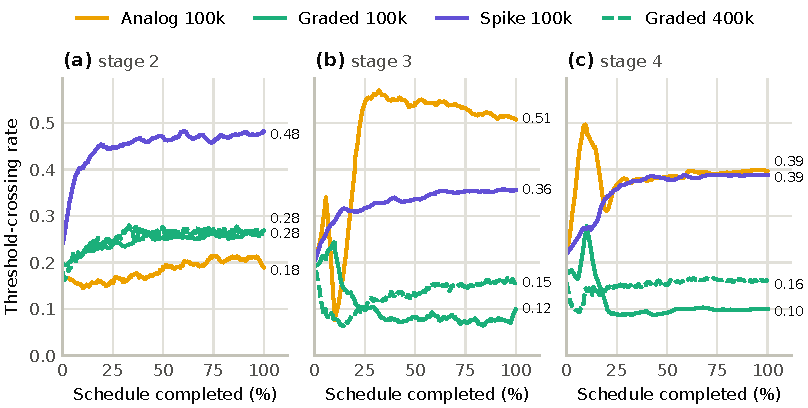
\includegraphics[width=\textwidth]{images/fig_spiking_firing.pdf}
    \caption[Readout firing rates during training]{Threshold-crossing rate of the LIF readout during training at spiking stages (a) 2, (b) 3 and (c) 4,
    from the training-time monitor, against the share of the schedule completed; 100k-step readouts solid,
    graded 400k-step run dashed. End labels are the final rates.}
    \label{fig:spiking_firing}
\end{figure}

\begin{figure}[htbp]
\centering
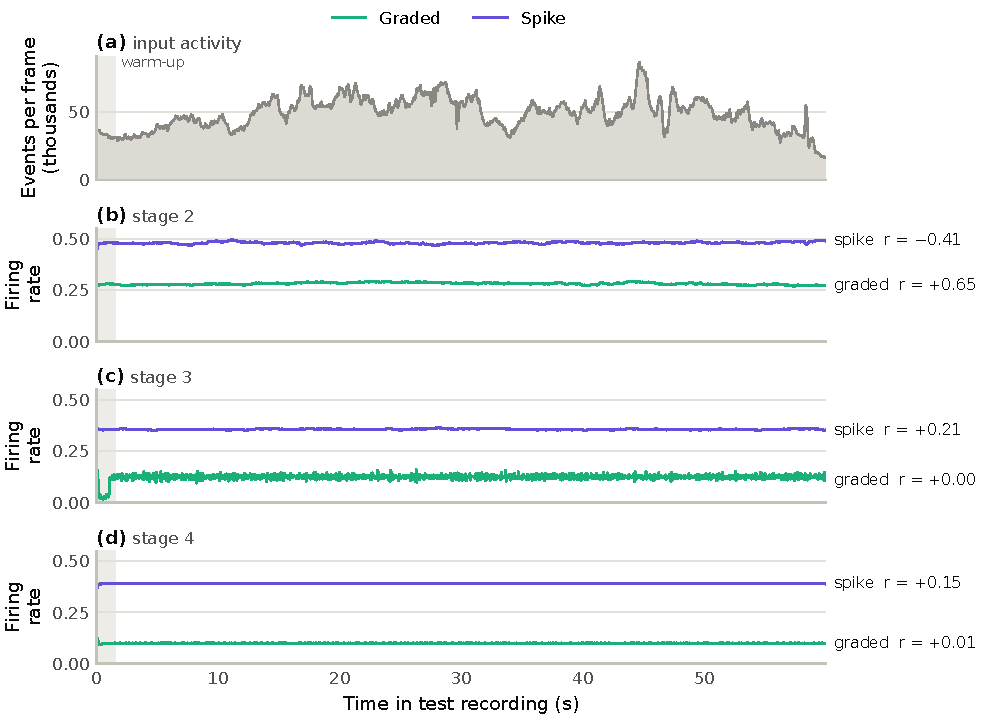
\includegraphics[width=\textwidth]{images/fig_firing_pattern.pdf}
\caption[Readout activity over one test recording]{The readouts' activity over one 60-s test recording (\texttt{18-03-29\_13-15-02}, 1{,}200 frames of
50\,ms), 100k-step graded and binary checkpoints. (a) Events per frame. (b)--(d) Share of nonzero readout outputs
at spiking stages 2, 3 and 4, on one shared scale; $r$ is the Pearson correlation with the events per frame. The
shaded first 32 frames, in which the recurrent state warms up from zero, are excluded from $r$.}
\label{fig:firing_pattern}
\end{figure}

\guide{150}{
  \item The threshold is fixed in training, so the trained weights can be re-run at other thresholds: post-hoc sensitivity, not a trained trade-off (Figure~\ref{fig:threshold_sweep}).
  \item The training threshold $\vartheta=1$ is the most accurate point for both readouts.
  \item Lower $\vartheta$: more firing, no gain (graded 40.68 at 21.1\,\% vs 40.72 at 17.3\,\%). Higher $\vartheta$: steep cost, faster for binary ($-2.3$ / $-11.8$ at 1.5 / 2 vs graded $-2.1$ / $-6.1$).
  \item Binary fires 2.4$\times$ as often as graded at $\vartheta=1$; even the sparsest point (5.3\,\%) would lift the saving only to about 0.99\,\%.
}
Because the threshold is fixed in training, the trained weights can be re-evaluated at other thresholds
(Figure~\ref{fig:threshold_sweep}); each point other than $\vartheta=1$ is a post-hoc operating point of the
same weights, so the curve measures sensitivity to the threshold rather than what a model trained at that
sparsity would reach. On both readouts the training threshold is the most accurate point. Lowering the
threshold raises the firing rate without gaining accuracy: at $\vartheta=0.75$ the graded readout drives
21.1 instead of 17.3\,\% of its spike-fed operations for 40.68 against 40.72~mAP. Raising it lowers the rate
at a steep cost, faster for the binary readout, which loses 2.3 and 11.8 points at $\vartheta=1.5$ and 2,
against 2.1 and 6.1 for the graded one. At the training threshold the binary readout fires 2.4 times as
often as the graded one. The threshold is also no energy lever on this architecture: even the sparsest
point measured (graded, $\vartheta=3$, 5.3\,\%) would raise the estimated saving of
Section~\ref{subsec:spk_energy} only from 0.86 to about 0.99\,\%, at a cost of 12.9 points.

\begin{figure}[htbp]
\centering
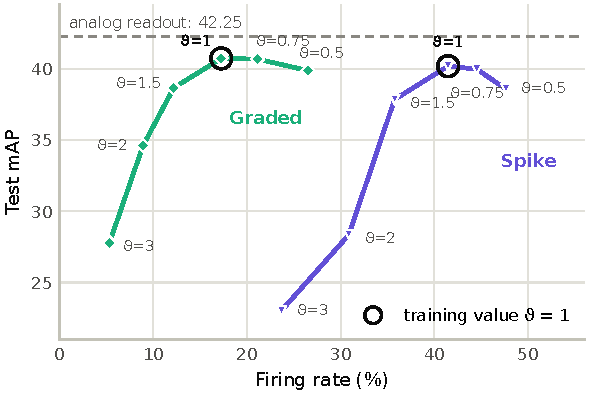
\includegraphics[width=0.75\textwidth]{images/fig_threshold.pdf}
\caption[Post-hoc threshold sensitivity]{Post-hoc threshold sensitivity of the 100k-step graded and binary readouts (Gen1 test set). Each point
re-evaluates the trained weights at another firing threshold; the ringed point is the training threshold
$\vartheta = 1$. Firing rate: share of the spike-fed neck operations driven. The dashed line is the dense analog
readout.}
\label{fig:threshold_sweep}
\end{figure}

\subsection{Rate Robustness of the Spiking Readouts}
\label{subsec:spk_rate}
\guide{60}{
  \item Same true-rate protocol, uncompensated; the leak and threshold were learned at the 50-ms rate only.
  \item Graded 400k retention at $10\times$: \res{\%} against 69.7\,\% for PureSSM 400k; at $2\times$: \res{\%}.
  \item Interpretation: does the LIF readout preserve, reduce or improve the robustness of the recurrence?
  \item If the 100k readouts were measured: their retention against the PureSSM 100k anchor.
}
Under the true-rate protocol of Section~\ref{subsec:eval_rob}, without compensation, the graded readout
trained on the full schedule retains \res{\%} of its accuracy at ten times the rate and \res{\%} at twice
the rate, against 69.7 and 95.9\,\% for PureSSM on the same schedule. Its leak and threshold were learned
at the 50-ms training rate only, so this measures whether the LIF readout preserves the robustness of the
uncompensated recurrence. \res{Interpret: preserved, reduced or improved; add the 100k readouts against
the PureSSM 100k anchor if measured.}

\subsection{Synaptic Operations and Estimated Energy}
\label{subsec:spk_energy}
\guide{110}{
  \item Table~\ref{tab:sop}: graded 400k drives 10.1 of the 52.4\,M spike-fed MACs $\Rightarrow$ 22.81 vs 23.01\,mJ per frame dense, a saving of 0.84\,\% (ceiling 1.04\,\%).
  \item The ladder's energy side: analog $-0.01$\,\%, graded 0.86\,\%, binary 0.96\,\% (an AC costs about a fifth of a MAC, so binary saves more despite firing 2.4$\times$ as often).
  \item Operation-count estimate; memory traffic not modelled.
}
Equation~\eqref{eq:sop_energy} turns the measured rates into an energy estimate (Table~\ref{tab:sop}). The
graded 400k-step readout drives 10.1 of the 52.4\,M spike-fed MACs per frame, which gives 22.81~mJ per
frame against 23.01~mJ for dense execution, a saving of 0.84\,\% against a ceiling of 1.04\,\%. The three
100k-step readouts give the energy side of the ladder: the dense analog readout saves nothing ($-0.01$\,\%
once the neuron updates are counted), the graded readout 0.86\,\% and the binary readout 0.96\,\%. The
binary readout saves slightly more although it fires 2.4 times as often, because an accumulate costs
about a fifth of a multiply--accumulate. These are operation counts with 45-nm constants; memory traffic,
which dominates energy on real hardware, is not modelled.

\begin{table}[htbp]
\centering
\caption[Operation-count energy estimate per readout]{Operation-count energy estimate per frame (Equation~\eqref{eq:sop_energy}; 45-nm constants,
$E_{\mathrm{MAC}} = 4.6$\,pJ, $E_{\mathrm{AC}} = 0.9$\,pJ~\cite{horowitz2014computing}). Rates: share of nonzero
readout outputs over 16 test clips after a 32-frame warm-up. Every arm has 52.4\,M spike-fed of 5.00\,G MACs
per frame, so the saving is capped at 1.04\,\%. Active inputs of a graded or analog readout carry a value and
are priced as multiply--accumulates (MAC), binary spikes as accumulates (AC). Memory traffic is not modelled.}
\label{tab:sop}
\small
\setlength{\tabcolsep}{3.5pt}
\begin{tabular}{lccccc}
\toprule
\textbf{Readout (priced as)} & \textbf{Nonzero rate, s2 / s3 / s4} & \textbf{Driven ops} & \textbf{mJ/frame} & \textbf{Dense} & \textbf{Saving} \\
\midrule
graded, 400k (MAC) & 0.263 / 0.140 / 0.157 & 10.1\,M & 22.81 & 23.01 & 0.84\,\% \\
analog, 100k (MAC) & 1.000 / 1.000 / 1.000 & 52.4\,M & 23.01 & 23.01 & $-0.01$\,\% \\
graded, 100k (MAC) & 0.257 / 0.125 / 0.100 & 9.0\,M & 22.81 & 23.01 & 0.86\,\% \\
binary, 100k (AC)  & 0.484 / 0.357 / 0.391 & 21.7\,M & 22.79 & 23.01 & 0.96\,\% \\
\bottomrule
\end{tabular}
\end{table}

\guide{90}{
  \item On the GPU (Table~\ref{tab:spiking_bench}, one session): 27.19 vs 26.46\,ms for PureSSM (+0.73\,ms for the LIF loop); state +1.1\,MB.
  \item GPU energy 0.55--0.69\,J (idle drift), overlapping PureSSM's 0.641\,J: no GPU energy difference claimed; dense kernels cannot exploit the sparsity.
}
On the GPU the spiking model brings no saving (Table~\ref{tab:spiking_bench}). Measured in one session with
the non-spiking models, it runs at 27.19~ms per frame against 26.46~ms for PureSSM, the extra 0.73~ms being
the loop over time steps of the LIF readout, and its streaming state is 1.1~MB larger. Its measured GPU
energy, 0.55--0.69~J per frame depending on how the drifting idle power is subtracted, overlaps PureSSM's
0.641~J, so no difference is claimed: dense GPU kernels do not exploit the readout's sparsity.

\begin{table}[htbp]
\centering
\caption[Benchmark of the graded readout and the non-spiking models]{The graded 400k-step SpikingSSM and the non-spiking models measured in one benchmark session
(harness of Table~\ref{tab:efficiency}, whose session gave 1--4\,\% higher latencies; models are compared within
a session only). $^{*}$The idle power drifted during these runs; the range spans subtraction of the idle power
measured before and after the run.}
\label{tab:spiking_bench}
\begin{tabular}{lcccc}
\toprule
\textbf{Metric} & \textbf{S5-RVT} & \textbf{EventSSM} & \textbf{PureSSM} & \textbf{SpikingSSM, graded} \\
\midrule
Parameters              & 18.19\,M & 19.18\,M & 16.33\,M & 16.34\,M \\
FLOPs                   & 11.06\,G & 12.71\,G & 10.03\,G & 10.03\,G \\
Latency p50, full       & 16.93\,ms & 12.09\,ms & 26.46\,ms & 27.19\,ms \\
Latency p50, backbone   & 10.41\,ms & 5.19\,ms & 19.64\,ms & 20.30\,ms \\
Energy per frame (GPU)  & 0.701\,J & 0.43--0.52\,J$^{*}$ & 0.641\,J & 0.55--0.69\,J$^{*}$ \\
Streaming state         & 4.7\,MB & 144.5\,MB & 144.5\,MB & 145.6\,MB \\
\bottomrule
\end{tabular}
\end{table}

\subsection{Training Dynamics}
\label{subsec:spk_dynamics}
\guide{110}{
  \item Binarisation slows learning: in the overfit gate, analog and graded reduce the loss 4.0$\times$ and 3.8$\times$ in 150 steps, binary 2.25--2.65$\times$ (passed at 300 steps, 4.95$\times$).
  \item Gradient test at stage 4: binary passes back 0.31$\times$ the analog gradient, graded 0.51$\times$.
  \item The learned leak barely moved: every channel within 0.044 of its 0.9 initialisation $\Rightarrow$ the Mamba recurrence upstream appears to do the integration.
}
Binarisation also slows learning. In the single-batch overfitting check that every model must pass, the
analog and graded readouts reduced the loss 4.0- and 3.8-fold within 150 steps, while the binary readout
reached only 2.25--2.65-fold in three runs and passed at 300 steps (4.95-fold). A gradient test isolating
stage~4 found that the binary readout passes back 0.31 times the gradient of the analog readout, and the
graded readout 0.51 times. The learned leak barely moved: on the final 100k-step checkpoints no channel lies
more than 0.044 from its initial value of 0.9. The Mamba recurrence upstream appears to supply the temporal
integration, leaving the membrane's own leak little to do.

\section{Summary of Results}
\label{sec:results_summary}
\guide{150}{
  \item One paragraph pulling the chapter together, in the order of the aims.
  \item Reproduction exact; PureSSM equal overall, +2.95 $\mathrm{AP}_L$, explained by a learned wider field; most rate-robust; compensation not reproducible; efficiency a trade-space; spiking costs dominated by sparsity, nearly free on the full schedule, energy saving bounded at about 1\,\%.
}
The baseline reproduced exactly, which validates every comparison that follows. Replacing the
convolutional spatial mixer with a state-space one left overall accuracy unchanged but raised large-object
accuracy by 2.95 points, and the receptive-field probe links that gain to a field that the state-space
mixer learns to make up to twice as wide. The state-space detectors kept 62--70\,\% of their accuracy at a
true tenfold rate, PureSSM the most, without the inference-time compensation, which lowered accuracy at
every tested point and whose published result could not be reproduced. Efficiency is a trade-space:
PureSSM needs the least computation but is the slowest on a GPU in eager execution, and both Mamba models
carry a streaming state 31 times the baseline's. The cost of spiking is dominated by sparsity rather than by
binarisation, nearly vanishes on the full schedule, and saves at most about 1\,\% of the detector's
operations, because the spikes reach only the first layers of the neck.

\chapter{Discussion}
\label{ch:discussion}

\section{Answering the Research Question}
\label{sec:answer_rq}
\guide{130}{
  \item Answer the main question in two or three sentences: with everything else fixed, the state-space spatial mixer leaves overall accuracy unchanged, improves large objects, is more rate-robust and needs the least computation, at a latency and memory cost on a GPU.
  \item Answer the second question: spiking costs 2.3 points at 100k, mostly sparsity, nearly nothing on the full schedule; the energy return is bounded at about 1\,\% on this hybrid.
}
The research question asked what the backbone's spatial mixer contributes when everything else is held
fixed. The answer is specific. Replacing a convolutional spatial mixer with a state-space one leaves
overall accuracy unchanged, improves the detection of large objects by about 3 points, makes the detector
the most robust of those tested to a true change in event rate, and reduces the computation per frame; it
pays for this in wall-clock latency on a GPU and, through Mamba's state expansion, in streaming memory. The
second question receives an equally specific answer. Making the temporal readout spike costs 2.3 points on
a short schedule, mostly through sparsity rather than binarisation, and almost nothing on the full
schedule, while its estimated energy return on this hybrid is bounded at about 1\,\% of the detector's
operations.

\guide{140}{
  \item Each aim: met, partly met or not met, with the evidence (aims 1--3, 5 and 6 met; aim 4 met; the Thesis~A system-integration aim descoped).
  \item Each hypothesis: H1 supported; H2 supported for the robustness, not reproduced for the compensation; H3 supported, with the dynamics step indistinguishable from zero.
}
All six aims were met. The baseline reproduced exactly (aim~1); the two detectors were built as controlled
swaps and compared overall, per class and by size (aim~2); the large-object difference was explained by a
receptive-field probe (aim~3); robustness was measured in both regimes, with and without compensation
(aim~4); efficiency was measured on every axis (aim~5); and the spiking variant decomposed the cost of
spiking (aim~6). Of the hypotheses, H1 is supported: the state-space mixer learns a wider field and detects
large objects better at equal overall accuracy. H2 is supported for the robustness of the recurrence but
not for the compensation, which lowered accuracy at every tested point under the published artefacts. H3
is supported: the ordering analog $\geq$ graded $>$ binary held, although the cost of the neuron dynamics
is not distinguishable from zero.

\section{What the State-Space Model Contributes}
\label{sec:what_shown}
\guide{110}{
  \item A pure state-space spatial backbone is viable: no attention, almost no local convolution, yet equal accuracy with the fewest parameters and FLOPs.
  \item Keep it in proportion: 1.3 below the attention baseline; trained with half its batch size.
}
The first contribution is evidence that a state-space mixer can serve as the spatial backbone of an event
detector, not only as its temporal core. PureSSM uses no attention, and apart from strided downsampling its
only local spatial mixing is a zero-initialised depthwise term in each block. It nonetheless matches the
convolutional hybrid on overall accuracy with the fewest parameters (16.33\,M) and the fewest FLOPs
(10.03\,G) of the three models. Two qualifications keep this in proportion: it remains 1.3~mAP below the
attention-based baseline, and the own models trained with half the baseline's batch size, so the size of
that gap is not fully attributable to the architecture.

\guide{130}{
  \item The receptive field is the lever: one controlled change raises $\mathrm{AP}_L$ by 2.95 while small and medium barely move; the probe and the class pattern (cars, not pedestrians) agree.
  \item The two designs are both legitimate: published detectors keep a conventional mixer on one axis (S5-RVT, SMamba~\cite{yang2025smamba}); PureSSM buys accuracy on large objects and robustness, EventSSM latency.
}
The second contribution is the mechanism. One controlled change, the spatial mixer, raised large-object
accuracy by 2.95 points while small- and medium-object accuracy barely moved ($+0.08$ and $+0.28$), and
the receptive-field probe explains the pattern: the state-space mixer learns a field up to twice as wide
as the convolutional stack's. The class-level result agrees, since the gain is in cars, the class with
large and close instances. Published state-space event detectors keep a conventional mixer on one of the
two axes, attention in space for S5-RVT~\cite{zubic2024state} and a ConvLSTM in time for
SMamba~\cite{yang2025smamba}. PureSSM shows that both axes can be state-space, buying large-object
accuracy, rate robustness and less computation at the price of latency on current GPUs, so the
convolutional hybrid remains the better choice where latency on conventional hardware binds.

\section{Temporal Robustness and the \texorpdfstring{$\Delta t$}{Delta t}-Rescaling Claim}
\label{sec:discuss_robustness}
\guide{120}{
  \item Robustness is built into the recurrence, not added by the compensation: 62--70\,\% retention at $10\times$ without any compensation; the compensation lowered accuracy everywhere under the published artefacts.
  \item The regime matters: at a fixed cadence the baseline degrades least at the sparse end; under a true rate change PureSSM is best.
  \item Mamba's input-dependent step gives at most a marginal edge over S5 (63.0 vs 62.2\,\%).
}
The robustness that makes state-space models attractive for event data is real, but under the published
artefacts it is built into the recurrence rather than added by the compensation credited with it. Every
state-space model kept 62--70\,\% of its accuracy at a true tenfold rate without any compensation, while
rescaling the step lowered accuracy at every tested point. The regime also matters: with a fixed cadence
and shorter windows the baseline degrades least at the sparse end, whereas under a true rate change
PureSSM degrades least. Mamba's input-dependent step, which might be expected to adapt to the rate by
itself, gives at most a marginal edge over S5: EventSSM retains 63.0\,\% against S5-RVT's 62.2\,\%, and
the two also differ in their spatial mixers. The decisive factor is recurrence as such rather than
selectivity.

\guide{80}{
  \item Practical consequence for a UAV: the event rate varies with flight speed; a state-space detector degrades gracefully, without per-rate tuning.
  \item What remains open: whether the compensation behaves differently under the unreleased preprocessing.
}
For a flying platform, whose event rate rises and falls with its own speed, the practical consequence is
that a state-space detector degrades gracefully at a rate it was not trained for, and needs no per-rate
tuning to do so. Whether the compensation behaves differently under the preprocessing used for the
published experiment, which was not released, cannot be determined from the released material, and the
conclusion here is limited to what that material supports.

\section{Efficiency Trade-offs}
\label{sec:discuss_efficiency}
\guide{170}{
  \item No single winner: FLOPs (PureSSM), latency and energy (EventSSM), streaming memory (S5-RVT).
  \item Why FLOPs and latency disagree: many small scan kernels are launch-bound; scans use the GPU less well than convolutions.
  \item Event sparsity is unused on a GPU; 144 vs 4.7\,MB of state.
  \item The binding constraint of a deployment decides the choice.
}
The efficiency results do not produce a single winner. PureSSM needs the least computation and has the
best accuracy per FLOP; EventSSM is the fastest and draws the least energy per frame; the baseline carries
by far the smallest streaming state. FLOPs and latency disagree because PureSSM's fourteen bidirectional
scans launch many small kernels, so its eager execution is bound by launch overhead rather than
arithmetic, and because state-space scans use the GPU less efficiently than the convolution kernels it was
built for. CUDA-graph replay recovers most of the overhead, which indicates that the gap is largely an
implementation property rather than an intrinsic one. Two costs are intrinsic, however. Event sparsity is
not exploited on a GPU, which processes every frame densely, and Mamba's state expansion makes the
streaming state 31 times the baseline's, a real cost on a memory-limited embedded platform. Which model
is most efficient therefore depends on the constraint that binds a given deployment, which is why the
thesis reports the frontier rather than a winner.

\section{Latency and the Choice of Window}
\label{sec:latency_window}
\guide{140}{
  \item With 50-ms windows, an event waits on average 25\,ms (up to 50) before entering a frame, and inference adds 13--27\,ms: the sensor's microsecond latency is not exploited; the detector updates at 20\,Hz.
  \item What the sensor still contributes: dynamic range, no motion blur within the 5-ms bins, sparse output.
  \item The window is a trade-off, not a fixed limit: at 5-ms windows (200\,Hz) the models keep 62--70\,\% without retraining, and CUDA graphs run near 200\,Hz.
}
Every model bins events into 50-ms windows, so its latency is set by the window and the computation
rather than by the sensor: an event waits on average 25~ms, and up to 50~ms, before it enters a frame, and
inference adds 13--27~ms on the test GPU. At this setting the microsecond latency of the event camera is
not exploited, and the detector updates no faster than a 20-Hz frame camera; the advantages that remain
are the sensor's dynamic range, the absence of motion blur within the 5-ms bins and its sparse output. The
window is, however, a trade-off rather than a fixed constraint. With 5-ms windows at 200\,Hz and no
retraining, the state-space models keep 62--70\,\% of their accuracy, and under CUDA-graph replay EventSSM
and PureSSM run at 210 and 181\,Hz, close to the rate such windows require.

\section{The Neuromorphic Case}
\label{sec:neuro_case}
\guide{130}{
  \item Three properties a GPU cannot exploit: neuromorphic chips compute only on spikes, so energy scales with activity~\cite{davies2021advancing}; a diagonal linear recurrence maps onto neurons (S4D on Loihi~2: about 1000$\times$ less energy than on a Jetson~\cite{meyer2024diagonal}); Loihi~2 supports graded spikes~\cite{orchard2021efficient}.
  \item Three gaps to silicon: Mamba's input-dependent decay; the non-spiking spatial backbone; Lava archived $\Rightarrow$ NIR~\cite{pedersen2024neuromorphic} as the export boundary~\cite{intel2026lava}.
}
The neuromorphic strand rests on properties that a GPU cannot exploit. Neuromorphic processors compute
only when spikes arrive, so their energy scales with activity rather than frame size~\cite{davies2021advancing};
the temporal core of the models here is a linear recurrence with a diagonal decay, which decomposes into
independent per-state updates, and Meyer et al.~\cite{meyer2024diagonal} mapped such a model onto Loihi~2,
measuring about 1000 times less energy than on a Jetson Orin Nano; and Loihi~2 supports graded spikes, the
hardware counterpart of the graded readout~\cite{orchard2021efficient}. Three gaps separate this model from
silicon: Mamba's decay changes with every input, the spatial backbone does not spike, and Intel archived
its Lava framework in May 2026~\cite{intel2026lava}, so the model is exported through the vendor-neutral
NIR format~\cite{pedersen2024neuromorphic}.

\guide{90}{
  \item What this hybrid can save is small by construction: spikes reach about 1\,\% of the operations (Figure~\ref{fig:spike_fed_ops}).
  \item Its value is the decomposition: it shows where a fully spiking design should spend effort (sparsity is the expensive property; graded spikes are cheap in accuracy).
  \item The energy case requires the spatial backbone to spike as well.
}
What the spiking readout of this thesis can save is small, and by construction rather than by result: its
spikes feed only the first convolutions of the neck, about 1\,\% of the detector's operations
(Figure~\ref{fig:spike_fed_ops}), so even a silent readout on hardware that skipped every inactive input
would save at most about 1\,\%. The value of this hybrid is therefore not energy but the decomposition. It
shows that, on a selective state-space core, the expensive property of spiking is sparsity rather than
binarisation, which tells a fully spiking design where to spend its effort. The energy case itself
requires the spatial backbone to spike as well (Section~\ref{sec:future_work}).

\begin{figure}[htbp]
    \centering
    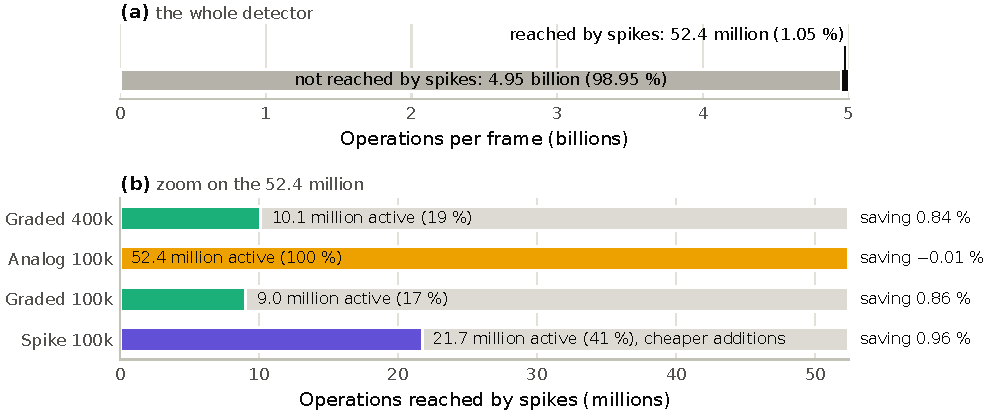
\includegraphics[width=\textwidth]{images/fig_spike_fed_ops.pdf}
    \caption[Share of operations reached by spikes]{How much of the detector's arithmetic the spikes reach. (a) Dense multiply--accumulates (MACs) per
    frame: the readout feeds only the first $1\times1$ convolutions of the neck, 1.05\,\% of the total. (b) Zoom
    on the spike-fed MACs: the share driven at each readout's measured nonzero rate (16 test clips, 32-frame
    warm-up) and the estimated saving of Equation~\eqref{eq:sop_energy} (operation counts with 45-nm constants;
    memory traffic not modelled), for the graded 400k-step readout and the three 100k-step readouts. Even a
    silent readout would save at most 1.04\,\%.}
    \label{fig:spike_fed_ops}
\end{figure}

\section{Scope Change: the Obstacle-Avoidance Aim}
\label{sec:scope_change}
\guide{50}{
  \item What was descoped: the Thesis~A aim of integration with an obstacle-avoidance controller in simulation and flight; also 1Mpx and embedded latency (Table~\ref{tab:aims}).
}
The fourth aim registered in Thesis~A, integration with an obstacle-avoidance controller in simulation and
physical micro-UAV testing if feasible, was not undertaken; two parts of the benchmarking aim, the 1Mpx
dataset and latency on embedded hardware, were also not delivered. Table~\ref{tab:aims} sets every
registered aim against what this thesis delivers.

\begin{table}[htbp]
\centering
\small
\caption[Thesis A aims against what was delivered]{Aims registered in Thesis~A against what was delivered.}
\label{tab:aims}
\begin{tabularx}{\textwidth}{@{}l>{\raggedright\arraybackslash}X>{\raggedright\arraybackslash}X@{}}
\toprule
\textbf{Aim} & \textbf{Registered} & \textbf{Delivered} \\
\midrule
1 Architecture & SSM detector, comparing S4/S5/Mamba variants &
  Delivered: two Mamba detectors (EventSSM, PureSSM) and a spiking variant, compared against the S5
  baseline (Chapter~\ref{ch:method}). \\
2 Benchmarking & Gen1 and 1Mpx; accuracy, latency, memory, energy; CNN, RNN and transformer baselines;
  embedded-hardware latency &
  Delivered on Gen1 with all four metrics (Sections~\ref{sec:acc_results}, \ref{sec:efficiency}); the
  RNN (ConvLSTM) baseline enters only through its published rate result.\needsgpu{decision D1: replace with
  the measured ConvLSTM baseline}
  1Mpx deferred to future work (Section~\ref{sec:future_work}); latency and energy measured on a
  desktop GPU, not embedded hardware. \\
3 Temporal generalisation & Inference at frequencies other than training, without retraining &
  Delivered and extended to two regimes, fixed cadence and true rate change, including a reproduction
  of inference-time $\Delta t$-rescaling (Section~\ref{sec:robustness}). \\
4 System integration & Obstacle-avoidance controller in simulation; micro-UAV flight if feasible &
  Descoped (this section). \\
\bottomrule
\end{tabularx}
\end{table}

\guide{150}{
  \item Why: the detector is trained on a car-mounted dataset; in a simulated UAV loop it would face unseen objects and viewpoints, so a collision rate would measure the domain gap, controller and simulator together, not the backbone.
  \item The aim also depended on assets outside the project's control (simulation plugins, stereo sensor, UAV hardware, approvals).
  \item What the effort produced instead; the SWaP motivation is unchanged, only the level of evaluation changed.
}
The descope follows from what a closed-loop demonstration could have measured. The detector is trained on
Gen1, recorded from a car, with car and pedestrian classes. Integrated in a UAV simulator it would face
objects and viewpoints it was never trained on, so a collision rate would have measured the domain gap,
the controller and the simulator together, and could not have isolated the contribution of the backbone,
which is the question this thesis sets out to answer. The aim also depended on assets outside the
project's control: event-camera simulation plugins, a stereo event sensor whose integration remained
unresolved, UAV hardware and flight approvals. The effort was redirected into the controlled study, which
produced the receptive-field mechanism, the two-regime robustness study and the efficiency frontier, none
of which a simulated demonstration would have yielded. The micro-UAV motivation is unchanged; what changed
is that the evaluation is architectural rather than system-level.

\section{Limitations}
\label{sec:limitations}
\guide{230}{
  \item Single unseeded runs: run-to-run variation unmeasured; only effects above about 1 point reported.
  \item One dataset with label noise; a fixed representation outside the ablation.
  \item Initialisation of the spatial mixers differs (ImageNet vs scratch); batch size and precision differ from the baseline.
  \item Spiking: energy is an estimate, not a measurement; the ladder uses a 100k schedule; resumed runs; threshold and surrogate not varied; the leak was little used.
}
The results carry the following limitations.
\begin{itemize}
  \item \textbf{Single runs.} Each model was trained once without a fixed seed, so run-to-run variation is
        unmeasured; overall differences below about 1~mAP are not treated as findings, and the larger
        effects also rest on single runs. The bootstrap intervals cover test-set sampling only.
  \item \textbf{One dataset.} All results are on Gen1: low resolution, an automotive viewpoint, two classes
        and incomplete labels, which cap the attainable AP. Generalisation to other resolutions, domains and
        lighting conditions is untested.
  \item \textbf{Fixed representation.} Every model inherits the stacked histogram, so the representation is
        not part of the ablation.
  \item \textbf{Initialisation and recipe.} EventSSM's ResNet-18 starts from ImageNet weights, while
        PureSSM is trained from scratch, so the comparison isolates the spatial mixer as instantiated,
        including its initialisation. Pre-training would be expected to favour the convolutional model. The
        own models also used half the baseline's batch size and bf16 precision, which affects only the
        comparison with the baseline.
  \item \textbf{Spiking model.} Its energy is an operation-count estimate with 45-nm constants, not a
        measurement on neuromorphic silicon, and memory traffic is not modelled. The ladder was trained on a
        100k-step schedule; the graded runs were resumed after interruptions, which changes their data
        order; the surrogate gradient and the training threshold were not varied; and the learned leak
        stayed close to its initial value, so the readout's own temporal dynamics were little used.
\end{itemize}

\section{Future Research Opportunities}
\label{sec:future_work}
\guide{210}{
  \item Four directions, one short paragraph or item each, in order of value.
  \item 1Mpx~\cite{perot2020learning}: does the large-object advantage grow with resolution? Posed as a falsifiable hypothesis (higher resolution adds temporal noise~\cite{gehrig2022high}); train on it, do not transfer zero-shot.
  \item Closed-loop evaluation on a UAV once a detector is trained on UAV-view data.
  \item Neuromorphic deployment on Loihi~2 via INRC and NIR; fixed-step decay.
  \item Toward a fully spiking detector (SiLIF-type neurons~\cite{fabre2025silif}) and activity-driven tokenisation~\cite{yang2025smamba}; the window latency study.
}
Four directions follow most directly from the results.
\begin{itemize}
  \item \textbf{High resolution.} Training on the 1Mpx dataset~\cite{perot2020learning}, with about 12.6
        times Gen1's pixel count, would test whether the large-object advantage of the state-space mixer
        grows with resolution. Because higher-resolution event cameras also produce more temporal
        noise~\cite{gehrig2022high}, the hypothesis is that rate-robust state-space detectors gain most from
        it; the models should be trained on the new data rather than transferred without retraining.
  \item \textbf{Closed-loop evaluation.} Once a detector is trained on data from a UAV's viewpoint, an
        avoidance controller can be evaluated by collision rate and avoidance latency, testing the
        prediction that the most rate-robust backbone degrades least as flight speed varies.
  \item \textbf{Neuromorphic deployment.} Running the spiking detector on Loihi~2 through the Intel
        Neuromorphic Research Community, exported through NIR, requires a fixed-step or on-chip form of the
        selective decay and a decision on where the non-spiking spatial backbone runs.
  \item \textbf{Fully spiking and event-driven designs.} Neurons whose state is itself a structured
        recurrence, such as SiLIF~\cite{fabre2025silif}, could make the temporal axis spiking end to end, and
        activity-driven tokenisation~\cite{yang2025smamba} could turn the event sparsity that a GPU ignores
        into saved computation. A sweep of the window from 50 to 5~ms, with fine-tuning, would map the
        latency--accuracy trade-off of Section~\ref{sec:latency_window}.
\end{itemize}

\chapter{Conclusion}
\label{ch:conclusion}
\guide{130}{
  \item Restate what was asked and how it was answered: a controlled study in which only the spatial mixer changes, on a verified baseline.
  \item The headline numbers: reproduction 47.72; 46.22 vs 46.43; $\mathrm{AP}_L$ +2.95 with a learned field up to twice as wide; 69.7\,\% retention; compensation not reproducible.
}
This thesis asked what a state-space model contributes to event-based object detection once everything
else in the detector is held fixed. It answered the question with a controlled study on a verified
baseline: S5-RVT reproduced exactly at 47.72~mAP, and two original detectors that differ only in their
spatial mixer were trained through the same unmodified pipeline. The convolutional EventSSM reached 46.22
and the state-space PureSSM 46.43~mAP, equal within single-run variation, but PureSSM detected large
objects 2.95 points better, and a receptive-field probe linked the gain to a field that the state-space
mixer learns to make up to twice as wide. PureSSM was also the most robust model tested to a true tenfold
change in event rate, keeping 69.7\,\% of its accuracy without the inference-time compensation, which, under
the published artefacts, lowered accuracy rather than raising it.

\guide{90}{
  \item The efficiency frontier in one sentence; the spiking decomposition in one sentence (costs, sparsity largest, nearly free at 400k, about 1\,\% energy bound).
}
The efficiency results form a frontier rather than a ranking: PureSSM needs the least computation, EventSSM
is the fastest and most energy-efficient on a GPU, and both Mamba models carry a streaming state 31 times
the baseline's. The spiking variant decomposed the cost of spiking on one membrane into the neuron
dynamics, sparsity and binarisation, $-0.28$, $-1.52$ and $-0.54$~mAP, with sparsity the only large step;
on the full schedule its graded readout came within 0.2 points of PureSSM, while its estimated energy
saving is bounded at about 1\,\% because the spikes reach only the first layers of the neck.

\guide{100}{
  \item The main limitation (single runs on one dataset) and the most important next step (a fully spiking or event-driven backbone, and evaluation beyond Gen1).
  \item One closing sentence on what the thesis establishes.
}
The main limitation is that every result rests on single runs on one low-resolution automotive dataset,
so the next steps are a second seed, training on high-resolution data, and a backbone whose spatial axis is
also event-driven, which is what the energy case for neuromorphic hardware requires. Within those limits,
the thesis establishes that a state-space model can serve as the spatial as well as the temporal mixer of
an event-camera detector, that its advantage lies where its learned receptive field predicts, and that its
efficiency must be judged against the constraint that binds a given deployment.

% ===================================================================== BACK MATTER (roman, continuing)
\clearpage
\pagenumbering{roman}
\setcounter{page}{\value{frontmatterpages}}

\phantomsection\addcontentsline{toc}{chapter}{\bibname}
\bibliographystyle{ieeetr}
\bibliography{references}

\appendix

\chapter{Mathematical Formulations}
\label{app:maths}

\section{Continuous-Time SSM}
\guide{30}{
  \item The continuous-time linear state-space model; define $u$, $h$, $y$, $A$, $B$, $C$, $D$.
}
A linear time-invariant state-space model maps an input signal $u(t)$ to an output $y(t)$ through a hidden
state $h(t)$, with a state matrix $A$, input matrix $B$, output matrix $C$ and direct feed-through $D$:

\begin{align}
    h'(t) &= A h(t) + B u(t) \\
    y(t) &= C h(t) + D u(t)
\end{align}

\section{Discretisation}
\guide{30}{
  \item Zero-order-hold discretisation with step $\Delta$ gives $\overline{A}$, $\overline{B}$, then the discrete recurrence.
  \item The step $\Delta$ is the quantity that inference-time rescaling changes.
}
With a zero-order hold over a step $\Delta$, the continuous model becomes the discrete recurrence below;
the step $\Delta$ is the quantity that the inference-time rescaling of Section~\ref{subsec:f2} changes.

\begin{align}
    \overline{A} &= \exp(\Delta A) \\
    \overline{B} &= (\exp(\Delta A) - I) A^{-1} B
\end{align}

\begin{align}
    h_k &= \overline{A} h_{k-1} + \overline{B} u_k \\
    y_k &= C h_k + D u_k
\end{align}

\section{Mamba Selective Scan}
\guide{40}{
  \item In Mamba the step and the projections are functions of the input; the full recurrence is Equation~\eqref{eq:mamba2_state}.
}
In a selective state-space model such as Mamba, the step and the input and output projections are
computed from the input at every step, so the decay $\exp(\Delta_k A)$ varies with the data; the Mamba-2
form used in this thesis is given in Equations~\eqref{eq:mamba2_state}--\eqref{eq:mamba2_out}.

\begin{equation}
    \Delta_k, B_k, C_k = f_\theta(u_k)
\end{equation}

\section{Event Representations}
\guide{20}{
  \item One sentence: the representation used, and the one planned in Thesis~A.
}
This section defines the representation used by every model and the one proposed in Thesis~A.

\subsection{Stacked Histogram}
\label{subsec:stacked_hist}
\guide{60}{
  \item Each event $k$ (time $t_k$, position $x_k, y_k$, polarity $p_k$) is assigned a bin $b_k$ within its window; counts per polarity and bin, capped at $c = 10$; channels stacked polarity-major (channel $pB+b$); stored as 8-bit integers.
}
Each event $k$ with timestamp $t_k$, position $(x_k, y_k)$ and polarity $p_k$ is assigned to one of $B=10$
bins of its window, and the events are counted per polarity, bin and pixel, with the count capped at
$c=10$. The two polarities and ten bins are stacked polarity-major into $2B = 20$ channels (channel
$pB+b$) and stored as 8-bit integers.

\begin{equation}
  b_k = \min\!\left(\left\lfloor B\,\frac{t_k - t_{\min}}{\max(t_{\max}-t_{\min},\,1)}\right\rfloor,\; B-1\right),
  \label{eq:sh_bin}
\end{equation}

\begin{equation}
  S_{p,b}(x,y) = \min\!\left(c,\; \sum_k \mathbb{1}[p_k=p]\,\mathbb{1}[b_k=b]\,\mathbb{1}[x_k=x]\,\mathbb{1}[y_k=y]\right).
  \label{eq:sh_count}
\end{equation}

\subsection{Voxel Grid (proposed in Thesis A; not used)}
\guide{40}{
  \item The voxel grid interpolates each event's signed polarity between neighbouring bins; proposed in Thesis~A, not used (Section~\ref{sec:repr}).
}
The voxel grid proposed in Thesis~A instead interpolates each event's signed polarity linearly between the
two nearest of $B$ bins. It was not used, because every model inherits the stacked histogram of the frozen
pipeline (Section~\ref{sec:repr}).

\begin{equation}
    V_b(x, y) = \sum_k p_k \cdot \max(0, 1 - |(B-1) \cdot t_k / T - b|) \cdot \delta(x-x_k) \cdot \delta(y-y_k)
\end{equation}

\chapter{Reproducibility}
\label{app:repro}
\guide{160}{
  \item Pinned environment in \texttt{env/} (Table~\ref{tab:env}); the runbooks in \texttt{docs/runbooks/}.
  \item Two pitfalls: install the Mamba kernels with \texttt{--no-deps}; set \texttt{TORCH\_FORCE\_NO\_WEIGHTS\_ONLY\_LOAD=1} to load Lightning checkpoints.
  \item The reference implementation is cloned at a pinned revision; every local change is kept as a patch; the evaluated checkpoints and their hashes (Table~\ref{tab:ckpts}); the test suite.
}
Everything needed to reproduce the results is in the project repository. The software environment is
pinned in \texttt{env/} (Table~\ref{tab:env}), and runbooks in \texttt{docs/runbooks/} cover environment
setup on a clean machine, re-running the baseline reproduction and training on a rented GPU. Two
environment pitfalls are documented there because they fail silently or confusingly: the Mamba kernels
must be installed without dependency resolution (\texttt{--no-deps --no-build-isolation}), since a default
install replaces PyTorch and breaks the Blackwell build, and loading full Lightning checkpoints under
PyTorch~2.6 or later requires \texttt{TORCH\_FORCE\_NO\_WEIGHTS\_ONLY\_LOAD=1}. The reference implementation
is cloned at a pinned revision, and every local change to it is stored as a patch and re-applied after a
re-clone; the frozen pipeline itself is not edited. The evaluated checkpoints are identified by their
hashes in Table~\ref{tab:ckpts}, and an automated test suite of about 500 tests checks the state handling,
the agreement of training and streaming evaluation, and the null test of the spiking model.

\begin{table}[htbp]
\centering
\small
\caption[Software environment]{Pinned software environment.}
\label{tab:env}
\begin{tabular}{ll}
\toprule
Component & Version \\
\midrule
Python & 3.11.15 \\
PyTorch & 2.11.0+cu128 (CUDA 12.8, Blackwell \texttt{sm\_120}) \\
\texttt{mamba-ssm} & 2.3.2.post1, built for \texttt{sm\_120} \\
\texttt{causal-conv1d} & 1.6.2.post1, built for \texttt{sm\_120} \\
PyTorch Lightning & 2.6.5 \\
Hydra & 1.3.2 \\
\texttt{torchdata} & 0.9.0 \\
Reference implementation & \texttt{ssms\_event\_cameras} at commit \texttt{7c871b5} \\
\bottomrule
\end{tabular}
\end{table}

\begin{table}[htbp]
\centering
\small
\caption[Checkpoints evaluated]{Checkpoints behind the reported results (SHA-256, first 16 hex digits).}
\label{tab:ckpts}
\begin{tabular}{llll}
\toprule
Model & Origin & Selected step & SHA-256 (prefix) \\
\midrule
S5-RVT & published release~\cite{zubic2024state} & --- & \texttt{58396f15b6c6081c} \\
EventSSM & run \texttt{8zotrwjw}, workstation & 320k (best val.) & \texttt{e94a36c2157bfea0} \\
PureSSM & run \texttt{aekvsalq}, rented RTX~5090 & 310k (best val.) & \texttt{a07c108b430d288a} \\
\bottomrule
\end{tabular}
\end{table}

\chapter{Project Timeline}
\label{app:timeline}
\guide{50}{
  \item The plan registered in Thesis~A (Table~\ref{tab:timeline}, Figure~\ref{fig:gantt}) against the timeline as executed (Figure~\ref{fig:gantt_actual}); the main deviation: the integration phases replaced by the controlled study and the spiking model.
}
Table~\ref{tab:timeline} and Figure~\ref{fig:gantt} show the plan registered in Thesis~A, and
Figure~\ref{fig:gantt_actual} the timeline as executed, reconstructed from the repository history. The main
deviation is that the simulation-integration and hardware-testing phases were replaced by the controlled
architectural study and the spiking model (Section~\ref{sec:scope_change}).

\begin{table}[htbp]
    \centering
    \caption[Planned timeline and milestones (Thesis A)]{Summary of the thesis timeline and major milestones, as registered in Thesis~A.}
    \label{tab:timeline}
    \renewcommand{\arraystretch}{1.4}
    \begin{tabularx}{\textwidth}{|l|X|l|}
        \hline
        \rowcolor[gray]{0.9} \textbf{Phase} & \textbf{Tasks} & \textbf{Timeline} \\ \hline
        Literature Review \& Foundations & Complete literature survey; identify optimal SSM variant and event representation. & Weeks 1--12 (Thesis A)  \\ \hline
        Architecture Design & Design SSM detection architecture; implement in PyTorch. & Weeks 13--16 (Thesis A/B)  \\ \hline
        Dataset Preparation & Download and preprocess Gen1/1Mpx datasets; implement data loaders. & Weeks 17--18 (Thesis B) \\ \hline
        Training \& Benchmarking & Train models; benchmark against baselines; ablation studies. & Weeks 18--22 (Thesis B)  \\ \hline
        Temporal Generalisation & Evaluate multi-frequency deployment; compare with RNN/Transformer. & Weeks 23--25 (Thesis B)\\ \hline
        Simulation Integration & Integrate with avoidance controller; evaluate in simulation. & Weeks 26--29 (Thesis B)\\ \hline
        Hardware Testing (if feasible) & Deploy on physical UAV platform; collect real-world results. & Weeks 30--33 (Thesis B/C)\\ \hline
        Thesis Writing & Complete thesis document; final revisions. & Weeks 34--40 (Thesis C)  \\ \hline
    \end{tabularx}
\end{table}

\begin{figure}[htbp]
    \centering
    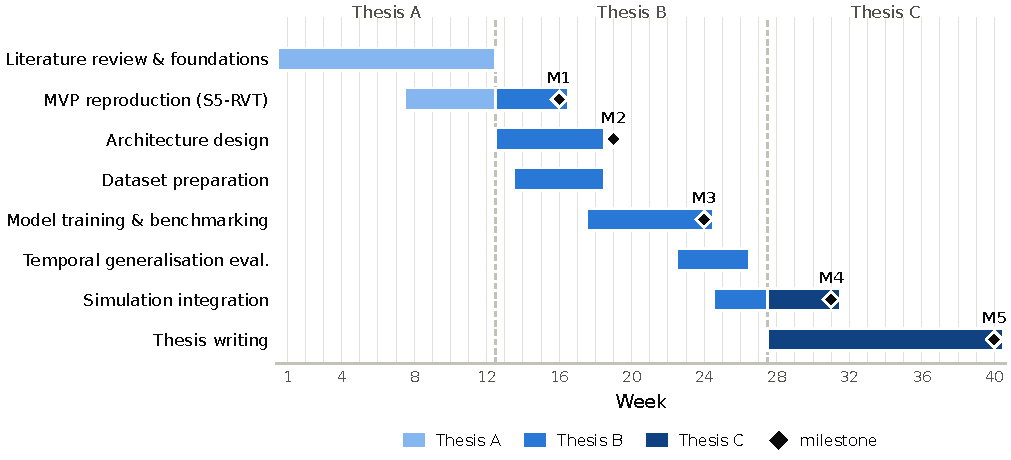
\includegraphics[width=\textwidth]{images/fig_gantt.pdf}
    \caption[Planned project timeline]{Project Gantt chart showing the week-by-week schedule across all thesis phases. Thesis~A (Weeks 1--12) covers the literature review and MVP baseline reproduction. Thesis~B (Weeks 13--27) covers architecture design, dataset preparation, model training and benchmarking, temporal generalisation evaluation, and simulation integration. Thesis~C (Weeks 28--40) covers thesis writing and final submission. Diamond markers (M1--M5) indicate key milestone deliverables. The chart and Table~\ref{tab:timeline} were prepared separately in Thesis~A and differ in some week ranges; both are reproduced as registered.}
    \label{fig:gantt}
\end{figure}

\begin{figure}[htbp]
    \centering
    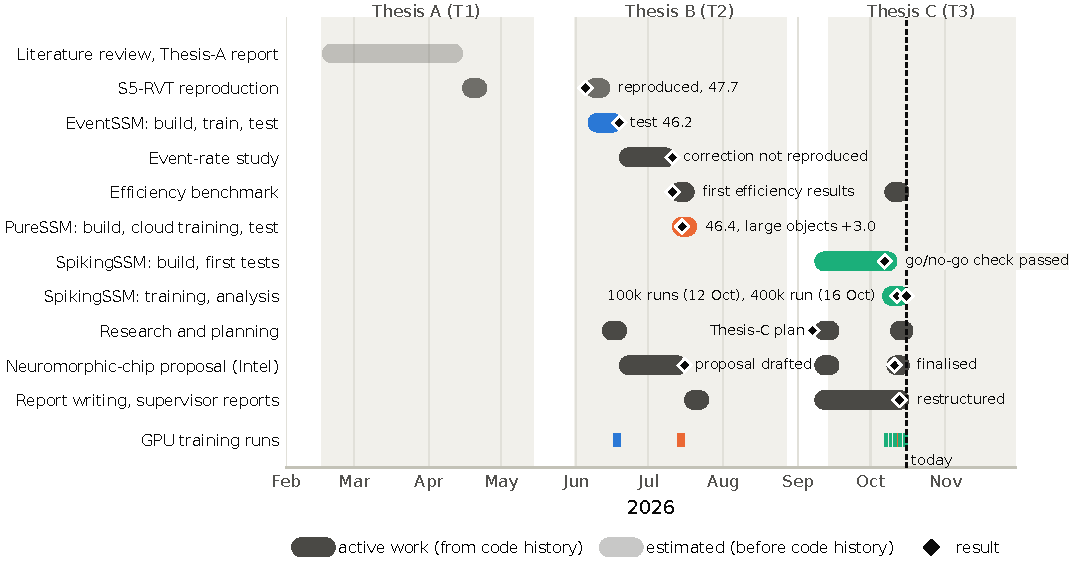
\includegraphics[width=\textwidth]{images/fig_gantt_actual.pdf}
    \caption[Project timeline as executed]{Project timeline as executed, February to November 2026, reconstructed from the repository history for comparison with the plan of Figure~\ref{fig:gantt}. Each bar is a work period of one stream, from its first to its last commit; a period continues through quiet spells of up to four weeks, and short bursts are drawn at least ten days long. The literature review before the first commit (15 April 2026) has no repository record and is shown as an inferred period. The bottom row shows the span of every training run, taken from the run logs (the two cloud PureSSM runs to day precision). Diamonds mark dated results; shading marks the three thesis terms (UNSW T1--T3 2026).}
    \label{fig:gantt_actual}
\end{figure}

\chapter{Risk Assessment}
\label{app:risk}
\guide{20}{
  \item The main risks of Thesis~C, their likelihood and impact, and how each was mitigated (Table~\ref{tab:risk_assessment}).
}
Table~\ref{tab:risk_assessment} lists the main risks of Thesis~C with their likelihood, impact and
mitigation, as assessed during the project.

\begin{table}[htbp]
    \centering
    \small
    \caption[Risk assessment]{Risk register for Thesis~C (status on 6 October 2026).}
    \label{tab:risk_assessment}
    \renewcommand{\arraystretch}{1.4}
    \begin{tabularx}{\textwidth}{|>{\RaggedRight\arraybackslash}p{3.2cm}|l|l|>{\RaggedRight\arraybackslash}X|}
        \hline
        \rowcolor[gray]{0.9} \textbf{Risk} & \textbf{Likelihood} & \textbf{Impact} & \textbf{Mitigation and status} \\ \hline
        Spiking model does not train stably & Medium & High & A kill-switch fixed before training: if the model is not training stably by 11~October, it is frozen as a simulated proof of concept and effort moves to the write-up. Spiking is introduced stage by stage, and the residual bypass is reported if used. \emph{Status:} criteria met. In overfitting tests the dense and graded readouts pass, and the binary readout, which receives about a third of the dense readout's gradient, passes with twice the steps. In 25k-step runs with spiking at stage~4 the spike and graded readouts reached 0.345 and 0.343 validation mAP against 0.351 for PureSSM under the same schedule, with no silent or saturated stage; runs with spiking at stages 2--4 are under way. \\ \hline
        Single-seed variance & High & Medium & Each model is trained once. Run-to-run variation is unmeasured; overall-mAP differences below about 1~mAP are treated as not distinguishable, and only larger effects, such as $\mathrm{AP}_L$ differences, are reported as findings, as single-seed results (Section~\ref{sec:limitations}). \\ \hline
        Training environment breaks & Medium & High & The hand-built Blackwell stack is pinned (Appendix~\ref{app:repro}); dependency resolution is disabled for the kernel packages; runbooks and patches rebuild it from scratch. \\ \hline
        Long run lost to a crash or out-of-memory kill & Medium & Medium & Full-state checkpoint resumption, validated in earlier runs; data-loader workers capped for host memory; a rented GPU of the same architecture as fallback. \\ \hline
        Write-up completed late & Medium & High & Writing runs in parallel with the experiments, and every non-spiking section is drafted before the spiking results arrive; the kill-switch caps the time the spiking strand can take. \\ \hline
        Neuromorphic hardware access delayed (INRC, Lava archived) & High & Low & Hardware deployment is future work, not a thesis result (Section~\ref{sec:future_work}); the model is exported through the vendor-neutral NIR format. \\ \hline
    \end{tabularx}
\end{table}

\end{document}
